%%
%% This is file `sample-sigconf-authordraft.tex',
%% generated with the docstrip utility.
%%
%% The original source files were:
%%
%% samples.dtx  (with options: `all,proceedings,bibtex,authordraft')
%% 
%% IMPORTANT NOTICE:
%% 
%% For the copyright see the source file.
%% 
%% Any modified versions of this file must be renamed
%% with new filenames distinct from sample-sigconf-authordraft.tex.
%% 
%% For distribution of the original source see the terms
%% for copying and modification in the file samples.dtx.
%% 
%% This generated file may be distributed as long as the
%% original source files, as listed above, are part of the
%% same distribution. (The sources need not necessarily be
%% in the same archive or directory.)
%%
%%
%% Commands for TeXCount
%TC:macro \cite [option:text,text]
%TC:macro \citep [option:text,text]
%TC:macro \citet [option:text,text]
%TC:envir table 0 1
%TC:envir table* 0 1
%TC:envir tabular [ignore] word
%TC:envir displaymath 0 word
%TC:envir math 0 word
%TC:envir comment 0 0
%%
%% The first command in your LaTeX source must be the \documentclass
%% command.
%%
%% For submission and review of your manuscript please change the
%% command to \documentclass[manuscript, screen, review]{acmart}.
%%
%% When submitting camera ready or to TAPS, please change the command
%% to \documentclass[sigconf]{acmart} or whichever template is required
%% for your publication.
%%
%%
\documentclass[sigconf,authordraft]{acmart}


\usepackage{hyperref}
\usepackage{url}
\usepackage{amsmath,amssymb,amsfonts}
\usepackage{algorithmic}
\usepackage{graphicx}
\usepackage{textcomp}
\usepackage{xcolor}
\usepackage{pifont} % for checkmark symbol
\usepackage{threeparttable}
\usepackage{tabularx}
\usepackage{booktabs}
\usepackage{rotating}
\usepackage{wrapfig}
\usepackage[subtle]{savetrees}
\usepackage{amsmath,amsfonts,amssymb,amscd,amsthm}
\usepackage{graphicx,xcolor,comment}
\usepackage{mathrsfs} 
\usepackage{calc}
\usepackage{multirow}
\usepackage{array}
\usepackage{hyperref}
\usepackage{multicol}
\usepackage{ragged2e}
\usepackage{pgfplots}
\pgfplotsset{compat=1.17}
\usetikzlibrary{pgfplots.groupplots}
% Define \sym for significance stars
\newcommand{\sym}[1]{^{#1}}
\usepackage{caption}
\usepackage[english]{babel}
\usepackage{rotating}
\usepackage{enumerate}
\usepackage{tikz}
\usepackage{bm}
\usepackage{csquotes}
\usepackage[useregional]{datetime2}
\usepackage{bbm}
\usepackage{tikz}
\usepackage{amssymb}
\usepackage{svg}
\usetikzlibrary{arrows.meta, positioning, decorations.pathreplacing}
\usepackage{amsmath}
\usepackage[export]{adjustbox}
\usepackage{mathrsfs}
\usepackage{booktabs}
\usepackage{threeparttable}
\usepackage{tabularx}
\usepackage{textcomp}
\usepackage{booktabs}
\usepackage{tabularx}
\usepackage{tikz}
\usetikzlibrary{shapes, arrows.meta, positioning, fit, backgrounds, calc, shadows}
\usetikzlibrary{shapes.geometric, arrows.meta, positioning, shadows, calc}
\usepackage{pgfplots}
\usetikzlibrary{arrows.meta, positioning, shapes.geometric}
\usepackage{amsmath}
\usepackage{tcolorbox}
\usepackage{xcolor}
\usepackage{etoolbox}
\usepackage{rotating}
\usepackage{booktabs}
\usepackage{threeparttable}
\usepackage{adjustbox}
\usepackage{eurosym}
\usepackage{booktabs}
\usepackage{longtable}
%-------- for bibliography -----------------
\usepackage{ amssymb }
\usetikzlibrary{positioning}
\usepackage{enumitem}
\usepackage{booktabs,longtable,array}
\pgfplotsset{compat=1.18}

% Define colors for visual mapping
\definecolor{isoBlue}{RGB}{0, 114, 178} % Decision variables
\definecolor{costRed}{RGB}{213, 94, 0}  % Objective
\definecolor{constrGreen}{RGB}{0, 158, 115} % Constraints

% Color Scheme
\definecolor{valBlue}{RGB}{0, 114, 178}   % Value Function / Future
\definecolor{profGold}{RGB}{230, 159, 0}  % Current Profit
\definecolor{stateGray}{RGB}{100, 100, 100} % State Variables

% --- ECONOMICS STYLE DEFINITIONS ---
% Define distinct, professional colors
\definecolor{econBlue}{RGB}{0, 107, 164}  % Demand
\definecolor{econRed}{RGB}{200, 82, 0}    % Supply
\definecolor{econGreen}{RGB}{89, 89, 89}  % Old equilibrium (Neutral)
\definecolor{econGold}{RGB}{255, 128, 14} % Transmission / Action
\definecolor{econBlue}{RGB}{31, 119, 180}
\definecolor{econRed}{RGB}{214, 39, 40}
\definecolor{econGold}{RGB}{188, 143, 46}

% Consistent Color Palette
\definecolor{fossilRed}{RGB}{204, 85, 0}   % Burnt Orange for Fossil
\definecolor{reGreen}{RGB}{0, 158, 115}    % Green for Renewables
\definecolor{noteGray}{RGB}{80, 80, 80}    % For notes

\definecolor{fossilRed}{RGB}{196, 69, 54}
\definecolor{fossilRedLight}{RGB}{248, 229, 227}
\definecolor{reGreen}{RGB}{46, 125, 50}
\definecolor{reGreenLight}{RGB}{232, 245, 233}
\definecolor{primaryBlue}{RGB}{26, 54, 93}
\definecolor{primaryBlueLight}{RGB}{232, 238, 245}
\definecolor{accentOrange}{RGB}{217, 119, 6}
\definecolor{mutedGray}{RGB}{73, 80, 87}
\definecolor{surfaceGray}{RGB}{248, 249, 250}

% Define consistent styles
\tikzset{
    econAxis/.style={thick, ->, >=stealth},
    supply/.style={thick, econRed},
    demand/.style={thick, econBlue},
    priceLine/.style={thin, gray, densely dashed},
}


\usetikzlibrary{intersections, decorations.pathreplacing, arrows.meta, calc, backgrounds}

% Define consistent colors (adjust these to match your presentation theme)
\definecolor{econBlue}{RGB}{31, 119, 180}
\definecolor{econRed}{RGB}{214, 39, 40}
\definecolor{econGold}{RGB}{188, 143, 46}

% Define consistent styles
\tikzset{
    econAxis/.style={thick, ->, >=stealth},
    supply/.style={thick, econRed},
    demand/.style={thick, econBlue},
    priceLine/.style={thin, gray, densely dashed},
}

%%
%% \BibTeX command to typeset BibTeX logo in the docs
\AtBeginDocument{%
  \providecommand\BibTeX{{%
    Bib\TeX}}}

%% Rights management information.  This information is sent to you
%% when you complete the rights form.  These commands have SAMPLE
%% values in them; it is your responsibility as an author to replace
%% the commands and values with those provided to you when you
%% complete the rights form.
\setcopyright{acmlicensed}
\copyrightyear{2018}
\acmYear{2018}
\acmDOI{XXXXXXX.XXXXXXX}
%% These commands are for a PROCEEDINGS abstract or paper.
\acmConference[Conference acronym 'XX]{Make sure to enter the correct
  conference title from your rights confirmation email}{June 03--05,
  2018}{Woodstock, NY}
%%
%%  Uncomment \acmBooktitle if the title of the proceedings is different
%%  from ``Proceedings of ...''!
%%
%%\acmBooktitle{Woodstock '18: ACM Symposium on Neural Gaze Detection,
%%  June 03--05, 2018, Woodstock, NY}
\acmISBN{978-1-4503-XXXX-X/2018/06}
\bibliographystyle{ACM-Reference-Format}


%%
%% Submission ID.
%% Use this when submitting an article to a sponsored event. You'll
%% receive a unique submission ID from the organizers
%% of the event, and this ID should be used as the parameter to this command.
%%\acmSubmissionID{123-A56-BU3}

%%
%% For managing citations, it is recommended to use bibliography
%% files in BibTeX format.
%%
%% You can then either use BibTeX with the ACM-Reference-Format style,
%% or BibLaTeX with the acmnumeric or acmauthoryear sytles, that include
%% support for advanced citation of software artefact from the
%% biblatex-software package, also separately available on CTAN.
%%
%% Look at the sample-*-biblatex.tex files for templates showcasing
%% the biblatex styles.
%%

%%
%% The majority of ACM publications use numbered citations and
%% references.  The command \citestyle{authoryear} switches to the
%% "author year" style.
%%
%% If you are preparing content for an event
%% sponsored by ACM SIGGRAPH, you must use the "author year" style of
%% citations and references.
%% Uncommenting
%% the next command will enable that style.
%%\citestyle{acmauthoryear}


%%
%% end of the preamble, start of the body of the document source.

%%% MACROS %%%
\newcommand{\nb}[1]{\textcolor{blue}{NB[#1]}}
\newcommand{\aruna}[1]{\textcolor{blue}{Aruna[#1]}}
\begin{document}

%%
%% The "title" command has an optional parameter,
%% allowing the author to define a "short title" to be used in page headers.
\title{An Econometric Model for Measuring Impacts of AI on United States Power Grids}

%%
%% The "author" command and its associated commands are used to define
%% the authors and their affiliations.
%% Of note is the shared affiliation of the first two authors, and the
%% "authornote" and "authornotemark" commands
%% used to denote shared contribution to the research.
% \author{Dana Golden}
% % \authornote{Both authors contributed equally to this research.}
% \email{dana.golden@stonybrook.edu}
% \orcid{1234-5678-9012}
% \affiliation{%
%   \institution{Stony Brook University School of Economics}
%   \city{Stony Brook}
%   \state{New York}
%   \country{USA}
% }

% \author{Aruna Balasubramanian}
% \affiliation{%
%   \institution{Stony Brook University School of Computer Science}
%   \city{Stony Brook}
%   \country{New York}}
% \email{arunab@cs.stonybrook.edu}

% \author{Niranjan Balasubramanian}
% \affiliation{%
%   \institution{Stony Brook University School of Computer Science}
%   \city{Stony Brook}
%   \country{New York}}
% \email{niranjan@cs.stonybrook.edu}



%%
%% By default, the full list of authors will be used in the page
%% headers. Often, this list is too long, and will overlap
%% other information printed in the page headers. This command allows
%% the author to define a more concise list
%% of authors' names for this purpose.
% \renewcommand{\shortauthors}{Golden, Balasubramanian, Balasubramanian}

%%
%% The abstract is a short summary of the work to be presented in the
%% article.
\begin{abstract}


Data centers now consume 4.4\% of U.S. electricity—more than double their 1.9\% share six years ago—yet AI's effects on grid stability remain poorly quantified. We exploit staggered Large Language Model releases as a natural experiment, using difference-in-differences to estimate how model training and inference affect local power grids. AI activity significantly degrades power quality and increases fossil fuel generation near data centers, with high-intensity periods \textbf{adding 0.5–1 outages per year.} We find an increase in fossil fuel power demand from AI \textbf{equivalent to $\sim$ 47,000 household-years} during inference.
We construct counterfactuals examining alternative AI development trajectories. \textbf{A 1\% increase in model parameters raises local power demand by 0.15\% post-release.} Fully implementing on-site generation would improve power quality by \textbf{0.17 reliability events per month—potentially making AI a net positive for grid reliability.}
% Data centers now account for 4.4\% of U.S. electricity demand, up from 1.9\% just six years ago, yet systematic quantification of AI's effects on grid stability remains limited. We exploit the staggered release of Large Language Models as a natural experiment, using difference-in-differences on a novel dataset to estimate how model training and inference affect local power grids. We find that AI activity significantly degrades power quality and increases fossil fuel generation near data centers, with high-intensity periods associated with 0.5–1 additional outages per year. Impact magnitude scales with model size.
% We construct counterfactuals examining alternative AI development trajectories including examinations of the role of model scaling in increasing energy usage, the impacts of colocated on-site generation, and the effects of a geographic redistribution of data centers used for AI. Our estimates show that larger models create significantly more grid strain with a \textbf{1\% parameter increase leading to an increase of .15\% higher power demand following model release}. Our estimates also show that \textbf{fully implementing across the board on-site generation would improve Consumer Power Quality Index by .17 reliability events per month and potential turn AI into a net positive for the grid.} We finally find that a shift to edge computing for inference dramatically lowers average increase in energy demand near data centers through redistribution while an increased concentration of training also concentrates higher energy burdens. Together, these results demonstrate that AI's grid effects are tightly coupled to both the technical trajectory of model development and the spatial organization of data-center infrastructure.
% We construct counterfactuals examining alternative AI development trajectories: transitioning from cloud to edge inference substantially mitigates grid impacts, as does relocating data centers to lower-density regions with greater energy availability. We further assess scenarios involving on-site generation colocated with the data center, local inference with smaller models, and plateauing training intensity. Using our regression estimates, we map efficiency improvements to grid impact reductions and quantify downtime costs to hyperscalers from spatial agglomeration. Together, these results demonstrate that AI's grid effects are tightly coupled to both the technical trajectory of model development and the spatial organization of data-center infrastructure.

% Data centers are a primary driver of modern power demand, a trend accelerated by Artificial Intelligence; in just six years, data center consumption grew from 1.9\% to 4.4\% of total U.S. power demand. Despite concerns regarding grid stability, systematic quantification of these effects remains limited. This paper utilizes the natural experiment of staggered Large Language Model (LLM) releases to perform a difference-in-differences analysis on a novel dataset, treating model training and inference as exogenous shocks to local power grids. We find that AI activity leads to significant degradation in power quality and increased fossil fuel generation near data centers. Specifically, high-intensity periods correlate with a localized reliability drop equivalent to an additional 0.5–1 power outages per year, with the magnitude of impact scaling with model size.

% We link model scale directly to impacts on electricity demand and power quality, and use these estimates to construct a set of counterfactuals that assess how alternative trajectories of AI development affect the power grid. We examine a transition from fully cloud-based inference to edge-based inference, finding that decentralization substantially mitigates grid impacts. We further quantify the potential benefits of relocating data centers toward regions with lower population density and greater energy availability. We rerun the estimates separately for data centers with and without behind-the-meter power generation and provide evidence on how grid impacts would change in a world where no data center or all data centers have behind-the-meter generation. Additional counterfactuals consider futures in which inference is primarily performed locally using smaller models, and in which growth in training intensity plateaus in the near term. Under stylized assumptions about inference costs based on our regressions, we provide sensitivity estimates that map percentage-scale improvements in model efficiency to reductions in grid impacts. Finally, we use public estimates of the costs of downtime by hyperscalers' cloud services to provide evidence of the costs to AI providers of increased potential for loss of service due to power outages due to significant spatial agglomeration in the data center industry. Together, these results show that AI’s effects on the power grid are tightly linked to both the technical trajectory of model development and the spatial organization of data-center infrastructure.
\end{abstract}

%%
%% The code below is generated by the tool at http://dl.acm.org/ccs.cfm.
%% Please copy and paste the code instead of the example below.
%%
\begin{CCSXML}
<ccs2012>
 <concept>
  <concept_id>10010520.10010553.10010562</concept_id>
  <concept_desc>Computer systems organization~Embedded and cyber-physical systems</concept_desc>
  <concept_significance>500</concept_significance>
 </concept>
 <concept>
  <concept_id>10010520.10010553.10010559</concept_id>
  <concept_desc>Computer systems organization~Reliability</concept_desc>
  <concept_significance>300</concept_significance>
 </concept>
 <concept>
  <concept_id>10010405.10010489</concept_id>
  <concept_desc>Applied computing~Energy management systems</concept_desc>
  <concept_significance>300</concept_significance>
 </concept>
 <concept>
  <concept_id>10010147.10010257</concept_id>
  <concept_desc>Computing methodologies~Machine learning</concept_desc>
  <concept_significance>100</concept_significance>
 </concept>
</ccs2012>
\end{CCSXML}

\ccsdesc[500]{Computer systems organization~Embedded and cyber-physical systems}
\ccsdesc[300]{Computer systems organization~Reliability}
\ccsdesc[300]{Applied computing~Energy management systems}
\ccsdesc[100]{Computing methodologies~Machine learning}

%%
%% Keywords. The author(s) should pick words that accurately describe
%% the work being presented. Separate the keywords with commas.
\keywords{Artificial intelligence, power grids, electricity markets, reliability, power quality, econometrics}
%% A "teaser" image appears between the author and affiliation
%% information and the body of the document, and typically spans the
%% page.
% \begin{teaserfigure}
%   
\includegraphics[width=\textwidth]{sampleteaser}
%   \caption{Seattle Mariners at Spring Training, 2010.}
%   \Description{Enjoying the baseball game from the third-base
%   seats. Ichiro Suzuki preparing to bat.}
%   \label{fig:teaser}
% \end{teaserfigure}

\received{20 February 2007}
\received[revised]{12 March 2009}
\received[accepted]{5 June 2009}

%%
%% This command processes the author and affiliation and title
%% information and builds the first part of the formatted document.
\maketitle

\section{Introduction}

\begin{figure}
    \centering
    %\vspace{-10pt}  
    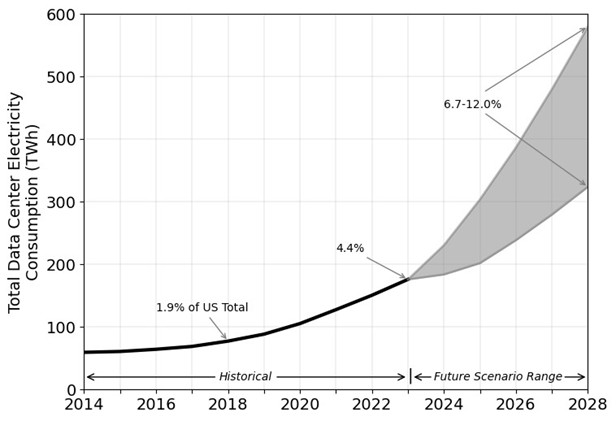
\includegraphics[width=.8\linewidth]{Figures/Data Center Electricity Consumption over Time (1).jpg}
    \caption{Projected data center growth over time. Source: DOE.}
    \label{fig:DataCenterGrowth}
    \vspace{-2pt}
\end{figure}

Over the past six years, data centers have expanded from consuming 1.9\% to 4.4\% of total U.S. electricity demand (Figure \ref{fig:DataCenterGrowth}, DOE). This rapid growth—driven largely by artificial intelligence—follows two decades of flat electricity consumption and coincides with nationwide efforts to electrify transport and heating. The combination poses a challenge: grid infrastructure was planned for stable demand, not simultaneous load growth from multiple sectors. Recent anecdotal evidence points to data centers reducing local power quality and raising prices \cite{Nicoletti_Malik_Tartar_2024}, yet systematic empirical evidence on these grid-level impacts remains scarce.

Existing work does not provide causal estimates of how AI deployments affect power systems at the {\em grid level}. Techno-economic assessments from international organizations broadly characterize rising AI workloads in the data center market \cite{RN1, RN3}. Micro-level studies examine energy performance of AI accelerators and identify workload management opportunities \cite{RN9, RN4}. A large computer science literature quantifies the compute, energy, and environmental costs of model development and deployment \cite{strubell19, schwartz2020green, RN7, RN5, morrison2025holistically}. These provide a foundation for understanding datacenter-level dynamics, but do not address the externalities experienced by other grid users—impacts on power quality, prices, and reliability that matter for energy security.

% However, systematic empirical evidence on these power-grid impacts remains scarce. Existing techno-economic assessments such as those from international organizations, and industry-focused reports~\cite{RN1, RN3} broadly highlight increasing share of AI workloads in the data center market. At the micro-level, some studies examine the energy performance of different AI accelerators and identify workload management opportunities for reducing power consumption\cite{RN9} and \cite{RN4}. Last, a vast body of computer science literature focuses on the compute, energy, and environmental costs of AI model development and deployment~\cite{strubell19,schwartz2020green,RN7, RN5, morrison2025holistically}. While these provide a strong basis for understanding how AI models impact datacenter level demand and efficiency opportunities, in this work we ask questions about the impact at the power-grid level with implications for energy reliability and security. %See~\autoref{sec:related-work} for a broader discussion.


%Energy consumption of AI models has received a lot of attention for its financial and environmental costs~\cite{} .  At a micro level, the AI community uses estimates of energy consumption of AI models for an instance and extrapolates to a data center level and the consequent environmental impacts (e.g. carbon footprints, embodied emissions) of training and deploying such models~\cite{}. At a macro level, the proliferation of data centers (e.g. DOE data shows demand rose from 1.9\% to 4.4\% of total U.S. electricity as in Figure \ref{fig:DataCenterGrowth}, DOE) and the ever increasing AI workloads in these, pose tremendous challenges to the power grids themselves. The huge loads cause fluctuations affecting power quality, and increasing demands, in conjunction with the increasing demand for renewables. 

Quantifying and understanding these power grid level impacts is critical from the perspectives of energy reliability and security. In this paper, we ask seek to answer four specific questions: 1) What are the effects of AI model releases on local power quality and power frequency? 2) How do AI training and inference affect electricity consumption around data centers owned by model developers? 3) How do these impacts translate into price effects in the wholesale and retail markets? Additional demand will likely increase prices, but understanding the magnitude of these price increases is important to determining the severity of the issue. 4) How will these impacts be different based on counterfactual scenarios articulating different technical evolutions of AI computing at scale? These scenarios include a shift away from cloud-based inference to edge-based computing, a geographic realignment of data centers away from population clusters, an evolution towards primarily inference-based or primarily training-based workloads, and a significant improvement in overall energy efficiency.

% \nb{I think we need to emphasize the challenge here a little more and play up our use of the idea and what were the issues we overcome in applying this idea or whatever else is interesting about its application to our specific problem.}
% It is challenging, however, to quantify these \emph{macro} grid-level impacts of AI models due to the lack of fine-grained data about other contributing factors that are unobservable due to proprietary aspects or otherwise prohibitively expensive to obtain. For example the power quality of a grid can be affected by many external factors including seasonal trends, location effects and data center internal factors such as other workloads which are unobservable proprietary information. 
One way to answer the above questions is to extrapolate from energy usage measurements (micro measures) within a datacenter to system-level (macro measures) impacts on the grid. This is however, is near infeasible because it requires a great deal of specific internal information that isolates what is run within the datacenter and when. While this data with level of detail is not available (for proprietary and other practical reasons), there are data sources that provide high-level observational data about various aspects of power consumption and quality at the grid-level over the time periods when models were trained and released. \emph{How can we answer specific questions about the impact of AI models with this high-level observational data alone?}

%In order to fully account for the energy usage and grid-level impacts of AI, we have to utilize variation within total energy usage and power quality at a grid level to perform natural experiments. This required the creation of a dataset combining data on energy and data centers in a novel way. Then, we developed an econometric model to exploit data on the dates of model training and inference. Finally, we ran extensive robustness tests to demonstrate the validity of the natural experiment. Our full methodology is described in Section \ref{Sec::Methods}.

We can draw upon econometric approaches for addressing this problem. In particular, we focus on the Difference-in-Differences (DiD) models which allows us to estimate the causal effects of AI model deployments on power systems, even when some contributing factors are unobservable. By comparing areas around data centers running AI models against control areas, and partitioning observations into pre- and post-release periods, we isolate AI-specific impacts while controlling for temporal and geographic factors. %We describe the DiD approach in more detail in Subsection \ref{EconometricModel}.

% \nb{I see many interesting things to say from the methods here. So much from 3.5 and 3.6 needs to be summarized here. Basically, you should sort of state the DiD as the high-level approach we can use but the key technical difficulties should be whatever that leads you to make the specific design choices within 3.5. The other fundamental technical difficulty is in ensuring that the underlying assumptions/validataions needed for identification, and robustness, which you lay out in 3.6. Can you try to take a stab at summarizing those? Something like the following but you should also add some stuff from 3.5}
% The key challenge in this approach is that the soundness of the DiD based inference depends on the strength of the evidence for the underlying \textit{parallel trends} assumption in our setting. \nb{Build our technical contributions for establishing this. You have put in a lot of careful thinking into the robustness checks. So lets highlight that.}

There are multiple technical challenges in applying this standard DiD approach in our setting: (i) There is a lack of specific information about when and where models are trained and released. Further model releases can be staggered, affecting the validity of the standard model which only uses one timepoint. (ii) The DiD method at its core relies on the parallel trends assumption i.e. we would know what would happen if the AI model were not run; in other words the estimates are valid only if we have a fairly accurate estimate of the trend of the variable of interest over time. (iii) There could be other confounding factors contributing to change in the variable of interest (e.g. extreme weather events coinciding with model release times could also cause increased power demand). (iv) No one clean dataset exists including all data useful for analysis. Often data are at different scales, lack linking tables, or require significant processing prior to use for analysis. In some cases, this requires significant efforts for manual mapping, combination, and labeling.
%\nb{This last point may not be the best characterization of the issue. Dana, please modify this as you see fit.} 

Our solution methodology addresses the above challenges:\\
\noindent \textbf{1) Addressing Inexact Information and Staggered Releases} %To address the issues of inexact information about AI model training and release times, 
We use a \textit{Staggered DiD} approach with multiple horizons, which has been used to overcome similar challenges in other applications ~\cite{cengiz2019effect, deshpande2019screened}. Staggered DiD with multiple horizons extends the standard two-period (pre/post), two-group setup to settings where treatment activates for different units at different times, leveraging this variation in rollout timing to assess different potential points of impact—analogous to how a staged feature rollout lets you compare early adopters against users still in the control group at each point in time.
%\aruna{Perhaps a one sentence explanation of staggered DiD and if we need to do anything special to get it to work?} 
For the question on fossil fuel demand effects, we address confounds such as alternative fuel prices or generator efficiency issues using a two stage regression, where we first factor out the impact of these confounds, and explain the remaining demand using a second stage staggered DiD. Similarly, for estimating price effects, we need to isolate effects from other sources of power demand that can cause price changes.
We handle confounds such as weather-driven and industry production driven shifts in demand (and thus price) via a two-stage regression. 

\noindent\textbf{2) Addressing validity of the DiD method and other confounds} We conduct a wide-array of statistical robustness checks supported by integration of large amounts of data from a diverse array of sources. We run statistical tests to show that we cannot reject the null hypothesis of parallel trends. We also run placebo tests with random treatment dates and randomized locations to show that our treatment effects are not the result of randomness, and we vary treatment definitions geographically and temporally. We use time series testing for anomaly detection and structural breaks to show that the differences we find in our regressions show up in model free analysis. Together, these robustness checks provide evidence of an experiment that is valid across all relevant dimensions.

\noindent\textbf{3) Addressing data disparity and relevance issues} 
%\nb{Dana to fix the following based on Aruna's comments.}
%(\aruna{how many?})
Training dates and facilities are generally unobserved, and for inference—which occurs continuously—these dates are not well-defined. We therefore rely primarily on model release dates. To strengthen identification, we supplement this with training locations, training dates, and API release dates gathered from press releases and news articles. We obtain verified training information for four models and confirmed API release dates for over half of the foundational models in our sample. We construct estimates using this most robust subset, then expand our model definitions to exploit exogenous variation for counterfactual analysis. Throughout, we use the most conservative feasible treated subset for each analysis. To construct suitable control groups, we employ propensity score matching as detailed in Appendix Subsection \ref{APP:PSM}, excluding observations without comparable pre-treatment trends.

%The key challenge in this approach is that the soundness of the DiD based inference depends on the strength of the evidence for the underlying \textit{parallel trends} assumption in our setting. Like any other experiment, the control and treatment groups must be comparable to establish validity. Any observed or unobserved sources of heterogeneity between groups that may impact the trend before or after treatment must be accounted for to ensure the results are trustworthy. Natural experiments are made exceedingly more complex by the inability to observe all details in all cases coupled with the inability to directly control selection criteria for treated observations before the fact. As such, we take great pains to provide thorough analysis to back up our claims of experimental validity.

%Because we do not observe the exact timeline of model training and inference in all cases, we primarily utilize a staggered DiD approach following \cite{cengiz2019effect} and \cite{deshpande2019screened}. The staggered DiD or \textit{event-study approach} is detailed in Subsection \ref{subsec:eventstudy}. In order to deal with the endogeneity of price effects, we use an two stage least squares instrumented design to map supply and demand curves. We find information from press releases and news articles on the training locations and training dates of models and dates of API release dates to create a conservative sample to demonstrate full robustness of the experiment under minimal assumptions. In order to develop a suitable control group, we take advantage of propensity score matching to cut samples that did not have comparable trends prior to the impacts of model training and inference.

%We also perform a series of robustness tests with methodology presented in Subsections \ref{subsec:robustness} and \ref{subsec:treatment} and results of robustness presented in Subsection \ref{Robustness} and the appendix. We run statistical tests to show that we cannot reject the null hypothesis of parallel trends. We run placebo tests with random treatment dates and randomized locations to show that our treatment effects are not the result of randomness, and we vary treatment definitions geographically and temporally. We use time series testing for anomaly detection and structural breaks to show that the differences we find in our regressions show up in model free analysis. Together, these robustness checks provide evidence of an experiment that is valid across all relevant dimensions.


% \nb{Say something about the reliability or trustworthiness of this data.}
We apply this methodology using publicly available data and proprietary on datacenter locations, power grid conditions, AI model release dates, and controls including weather and market prices. Our data creation process is described in detail in Section \ref{sectionData}. While all data pre-exist our analysis, the combination of the data creates a novel dataset that represents a significant contribution. Because the data are from government agencies, ISOs, or proprietary datasets, the data are highly trustworthy. We perform data validation to verify this. We estimate DiD models for outcomes measuring both power quality and electricity demand.

% \nb{Our findings speak to the large magnitude impacts of AI data centers.}
Our findings presented in Section \ref{Sec::Results} speak to the large magnitude of the impacts of AI data centers and the increasing effects of training ever-larger models over time. We find that large model releases (including the likes of GPT-3, Claude 2.1, Llama 2 documented in~\autoref{appendix:verified-models}) 
%\nb{I added these so people know what kinds of models are in our dataset. If it is inaccurate please fix.} DG: Looks good. I like the add. 
cause significant power quality deterioration in nearby areas -- \textbf{well above half the standard deviation of U.S. power-quality distributions}-- and increase fossil fuel consumption on the order of terawatt-hours--- \textbf{equivalent to around 45,000 households annual consumption}-- in both training and inference phases. We also find \textbf{wholesale electricity prices increase in treated PJM zones with increases of 25\%} during treatment in the American Electric Power (AEP) PJM Zone.
%\aruna{some is a bit vague}
%\nb{play up the counterfactuals some more.}
% These estimates enable counterfactual projections of how alternative technical trajectories would affect grid stability and energy consumption.
Using these estimates, we show in Subsection \ref{sec:counterfactuals} how altering the trajectory of AI along disparate dimensions impacts the grid. We are able to provide evidence for the separate impacts of training and inference, the effects of a shift to edge computing or more concentrated training loads, and how differential efficiency improvements impact AI's effects on power usage. We also show compelling evidence that significantly increasing on-site power generation provides a promising avenue for future reductions in grid impact.

This work makes three contributions. First, we develop a methodology for assessing macro-level grid impacts of AI models using publicly available data, even when fine-grained operational information is unavailable. Second, we provide the first causal estimates of these impacts for major frontier models, complementing the emerging literature on environmental and system-level effects of AI data centers \cite{murino2023sustainable, guidi2024environmental, thangam2024impact}. Finally, we provide policy-relevant counterfactual estimates for the impacts of technical evolution of AI on the grid.

%Over the past six years, data centers have expanded from consuming 1.9\% to 4.4\% of total U.S. electricity demand (Figure \ref{fig:DataCenterGrowth}, DOE). This rapid growth—driven largely by artificial intelligence—follows two decades of flat electricity consumption and coincides with nationwide efforts to electrify transport and heating. Together, these trends are straining the power grid and raising concerns about both reliability and affordability. Recent anecdotal evidence, such as \cite{Nicoletti_Malik_Tartar_2024}, points to data centers reducing local power quality and raising prices. Yet, systematic empirical evidence on these impacts remains scarce.

 %\aruna{we should align this with the three questions we ask in Section 4}

%To answer these questions, we combine econometric analysis of market data with techno-economic modeling of AI workloads. This dual approach allows us to move beyond carbon-intensity metrics and instead provide the first empirical estimates of AI’s impact on electricity demand and power quality near data centers. We then link these estimates to technical scenarios of AI efficiency gains, enabling counterfactual projections of their effects on energy consumption and grid stability. In doing so, our work contributes to the emerging literature on the environmental and system-level impacts of AI data centers \cite{murino2023sustainable,guidi2024environmental,thangam2024impact}, offering new insights into both environmental quality and energy security.
% The paper is organized as follows. Section 1 reviews the literature related to data center power usage. Section 2 describes the structure of the data center market and presents descriptive statistics power consumption by data centers and the impact of AI on data center power consumption. Section 3 presents a model of data center power procurement while Section 4 describes the methodology for the estimation of models related to answering the research question. Section 5 provides a description on results and model-fit. Section 6 details counterfactuals related to the impact of reducing AI power consumption on power quality. Section 7 details future research and concludes the paper.
\section{Related Work}

This paper contributes to four interrelated literatures. First, techno-economic assessments document the scale of data center electricity demand: Lawrence Berkeley estimates U.S. data center consumption could reach 6.7--12\% of national electricity by 2028 \cite{shehabi2024}, while utility five-year peak demand forecasts jumped from 38 GW to 128 GW between 2023 and 2024, with approximately 90 GW attributable to data centers \cite{gridstrategies2025}. Recent simulation studies examine AI-driven load growth implications for grid planning \cite{lin2024exploding, chien2023adapting}, but these assessments characterize aggregate trends rather than isolating causal mechanisms.

Second, computer science research quantifies AI's computational and environmental costs, from training emissions \cite{strubell19, schwartz2020green} to debates over efficiency improvements \cite{RN2, RN8} and inference-time scaling \cite{kim2025cost}, including data center carbon emissions \cite{datacenter-carbon}. Related work has developed carbon intensity forecasting methods \cite{maji2022dacf, li2023gnn} and examined power forecasting for grids \cite{optimizing-grid, carbon-intensity-forecasting}, but not in the context of AI workload impacts on market outcomes. Recent empirical projections analyze the tension between AI energy growth and grid decarbonization \cite{maji2024crossroads}, while others consider grid planning for AI demand \cite{ai-grid-planning}, yet the causal effect of AI deployment on wholesale markets remains unstudied.

Third, emerging evidence points to grid-level externalities from data center concentration. Sensor data reveals spatial correlation between data center proximity and power quality degradation \cite{nicoletti2024}, PJM capacity prices increased from \$30 to \$270/MW-day between 2023--2024 amid data center load growth \cite{cmu2025}, and transmission costs are increasingly socialized across ratepayers \cite{jacobs2025}. The systems literature has examined carbon-aware geographical load shifting using locational marginal prices \cite{lindberg2021guide} and data center demand response participation \cite{chen2019datacenter, liu2014pricing, klingert2018mapping}. These studies establish correlational patterns or propose optimization frameworks but lack causal identification.

Fourth, the econometric literature on electricity markets provides methodological foundations, including difference-in-differences for demand responses \cite{roth2024did} and event studies for policy interventions \cite{pnnl2022}, but has not applied quasi-experimental methods to AI deployment impacts.

We address this gap by treating AI model releases as plausibly exogenous demand shocks, using difference-in-differences to estimate causal effects on locational marginal prices and power quality. Unlike prior work building from computational requirements or facility audits, we analyze grid-level impacts using wholesale market data, capturing realized demand effects without requiring proprietary operational information.

% This paper contributes to four interrelated literatures. First, techno-economic assessments document the scale of data center electricity demand: Lawrence Berkeley estimates U.S. data center consumption could reach 6.7–12\% of national electricity by 2030 \cite{shehabi2024}, while utility five-year peak demand forecasts jumped from 38 GW to 128 GW between 2023 and 2024, with approximately 90 GW attributable to data centers \cite{gridstrategies2025}. These assessments characterize aggregate trends but do not isolate causal mechanisms.

% Second, computer science research quantifies AI's computational and environmental costs, from training emissions \cite{strubell19, schwartz2020green} to debates over efficiency improvements \cite{RN2, RN8} and inference-time scaling \cite{kim2025cost}, including data center carbon emission~\cite{datacenter-carbon}. This literature focuses on model- or facility-level accounting rather than system-wide market effects.  Related works have also examined power  forecasting for grids and effect of end-user incentives on grids~\cite{optimizing-grid,carbon-intensity-forecasting} but not in the context of AI workloads. More recently, researchers have begun to consider grid planning and management in the context of AI-driven electricity demand \cite{ai-grid-planning} but the effect of AI workload on power grids is still unstudied. 


% Third, emerging evidence points to grid-level externalities from data center concentration. Sensor data reveals spatial correlation between data center proximity and power quality degradation \cite{nicoletti2024}, PJM capacity prices increased from $30 to $270/MW-day between 2023–2024 amid data center load growth \cite{cmu2025}, and transmission costs are increasingly socialized across ratepayers \cite{jacobs2025}. These studies establish correlational patterns but lack causal identification.

% Fourth, the econometric literature on electricity markets provides methodological foundations, including difference-in-differences for demand responses \cite{roth2024did} and event studies for policy interventions \cite{pnnl2022}, but has not applied quasi-experimental methods to AI deployment impacts.

% We address this gap by treating AI model releases as plausibly exogenous demand shocks, using difference-in-differences to estimate causal effects on locational marginal prices and power quality. Unlike prior work building from computational requirements or facility audits, we analyze grid-level impacts using wholesale market data, capturing full demand effects without requiring proprietary operational information.

% \section{Background: Datacenter Concentration and Power-Quality}
% % \nb{One possibility is to roll this in with the problem definition in 3.1 if we need space.}
% % \nb{We should also have related work in terms of what kinds of analysis has been done and explain what our work contributes hasnt been done or not easily inferrable from existing work.}
% The U.S. data centers are expanding rapidly, nearly tripling from its 2008 levels to 1489 active sites in 2025, with another 1,359 on the horizon~\cite{aterio_us_data_centers_2025}. The market is dominated by \emph{hyperscalers}---vertically integrated datacenters---owned by AI heavy companies such as Amazon, Microsoft, and Google, alongside a long tail of smaller operators. Hyperscalers afford companies certain economies of scale but greatly increase the geographic concentration of power demand on the grids. Concentrated demand strains local grids in the area, raising congestion costs and sometimes degrading power quality for neighboring consumers. Large, inflexible loads from AI hyperscalers also reduce system reliability, elevate wholesale prices, and complicate renewable integration.
%\niranjan{These paragraphs can be compressed to state the problem more succinctly. Datacenters are concentrated in geographic locations because they provide certain benefits that come from economies of scale. This while has some economic benefits also brings in infrastructural impacts. We could even change the title of the section to: Background: Datacenter Concentration and Power-Quality Impact. End this section with questions on what to do about this.}
%\niranjan{Then move the Data sub-section to Methodology Section.}
%\subsection{Market Overview}

%The U.S. data center market has expanded rapidly, growing from 519 facilities in 2008 to 1,489 active sites in 2025, with another 1,359 announced or under construction \cite{aterio_us_data_centers_2025}. Electricity demand more than tripled over this period, rising from under 5 to over 15 GWh per hour (BNEF), while total U.S. capacity increased only 17.6\% \cite{EIA_2023_table4_2A} and dispatchable baseload capacity fell as coal retired.
% \niranjan{Renewable generation is not something we touch upon in the rest of the paper. Should we drop this reference? It would be better to talk about power generation and power demand in general.}
% Power consumption has risen in parallel, though since 2018 growth in renewable generation has outpaced data center demand as shown in Figure \ref{fig:DCPowerConsumption}.

% \begin{wrapfigure}{l}{0.45\linewidth}
%     \centering
%     \vspace{-10pt}
%     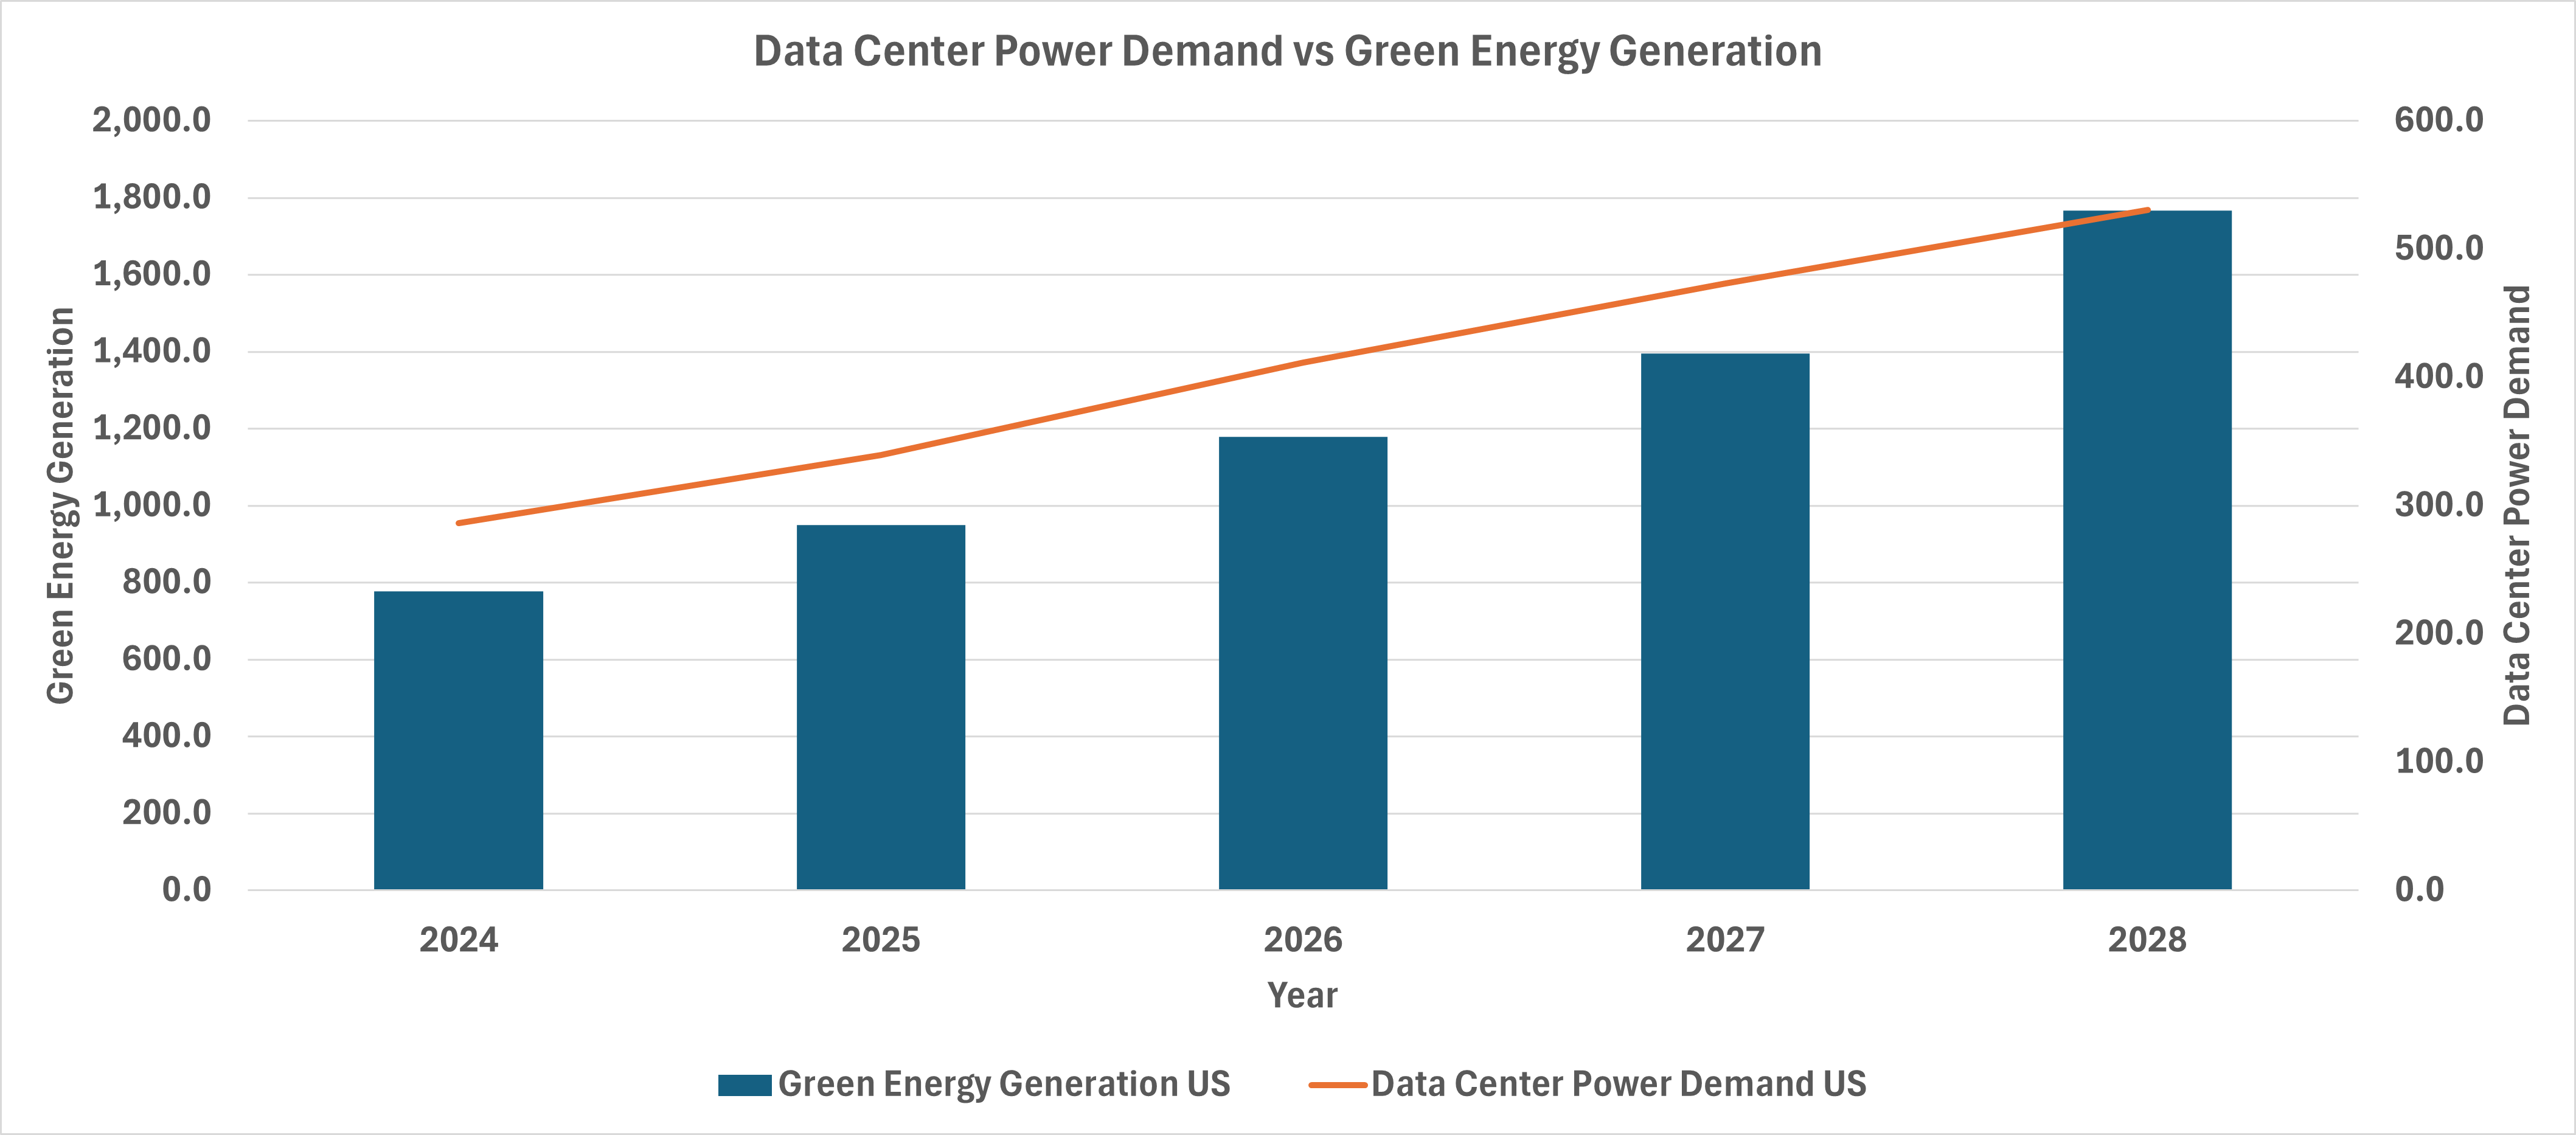
\includegraphics[width=\linewidth]{Figures/Data Center Power Demand vs Green Generation.png}
%     \caption{Data center power consumption vs.\ green generation. Source: Aterio.io.}
%     \label{fig:DCPowerConsumption}
%     \vspace{-10pt}
% \end{wrapfigure}

%The market is geographically concentrated and dominated by hyperscalers—Amazon, Microsoft, and Google—who account for 38\% of capacity across five firms, and 64\% across twenty. Unlike colocation providers such as Equinix, hyperscalers are vertically integrated, owning facilities, long-term power contracts, fiber networks, and custom chips. These economies of scale lower costs but also create externalities: concentrated demand strains local grids, elevates congestion, and reduces reliability, though clustering also generates jobs, tax revenue, and services. Given hyperscalers’ role in AI training and their outsized grid impacts, our analysis focuses on them.


% \begin{figure}[t!]
%     \centering
%     % First figure
%     \begin{minipage}[t]{0.45\linewidth}
%         \centering
%         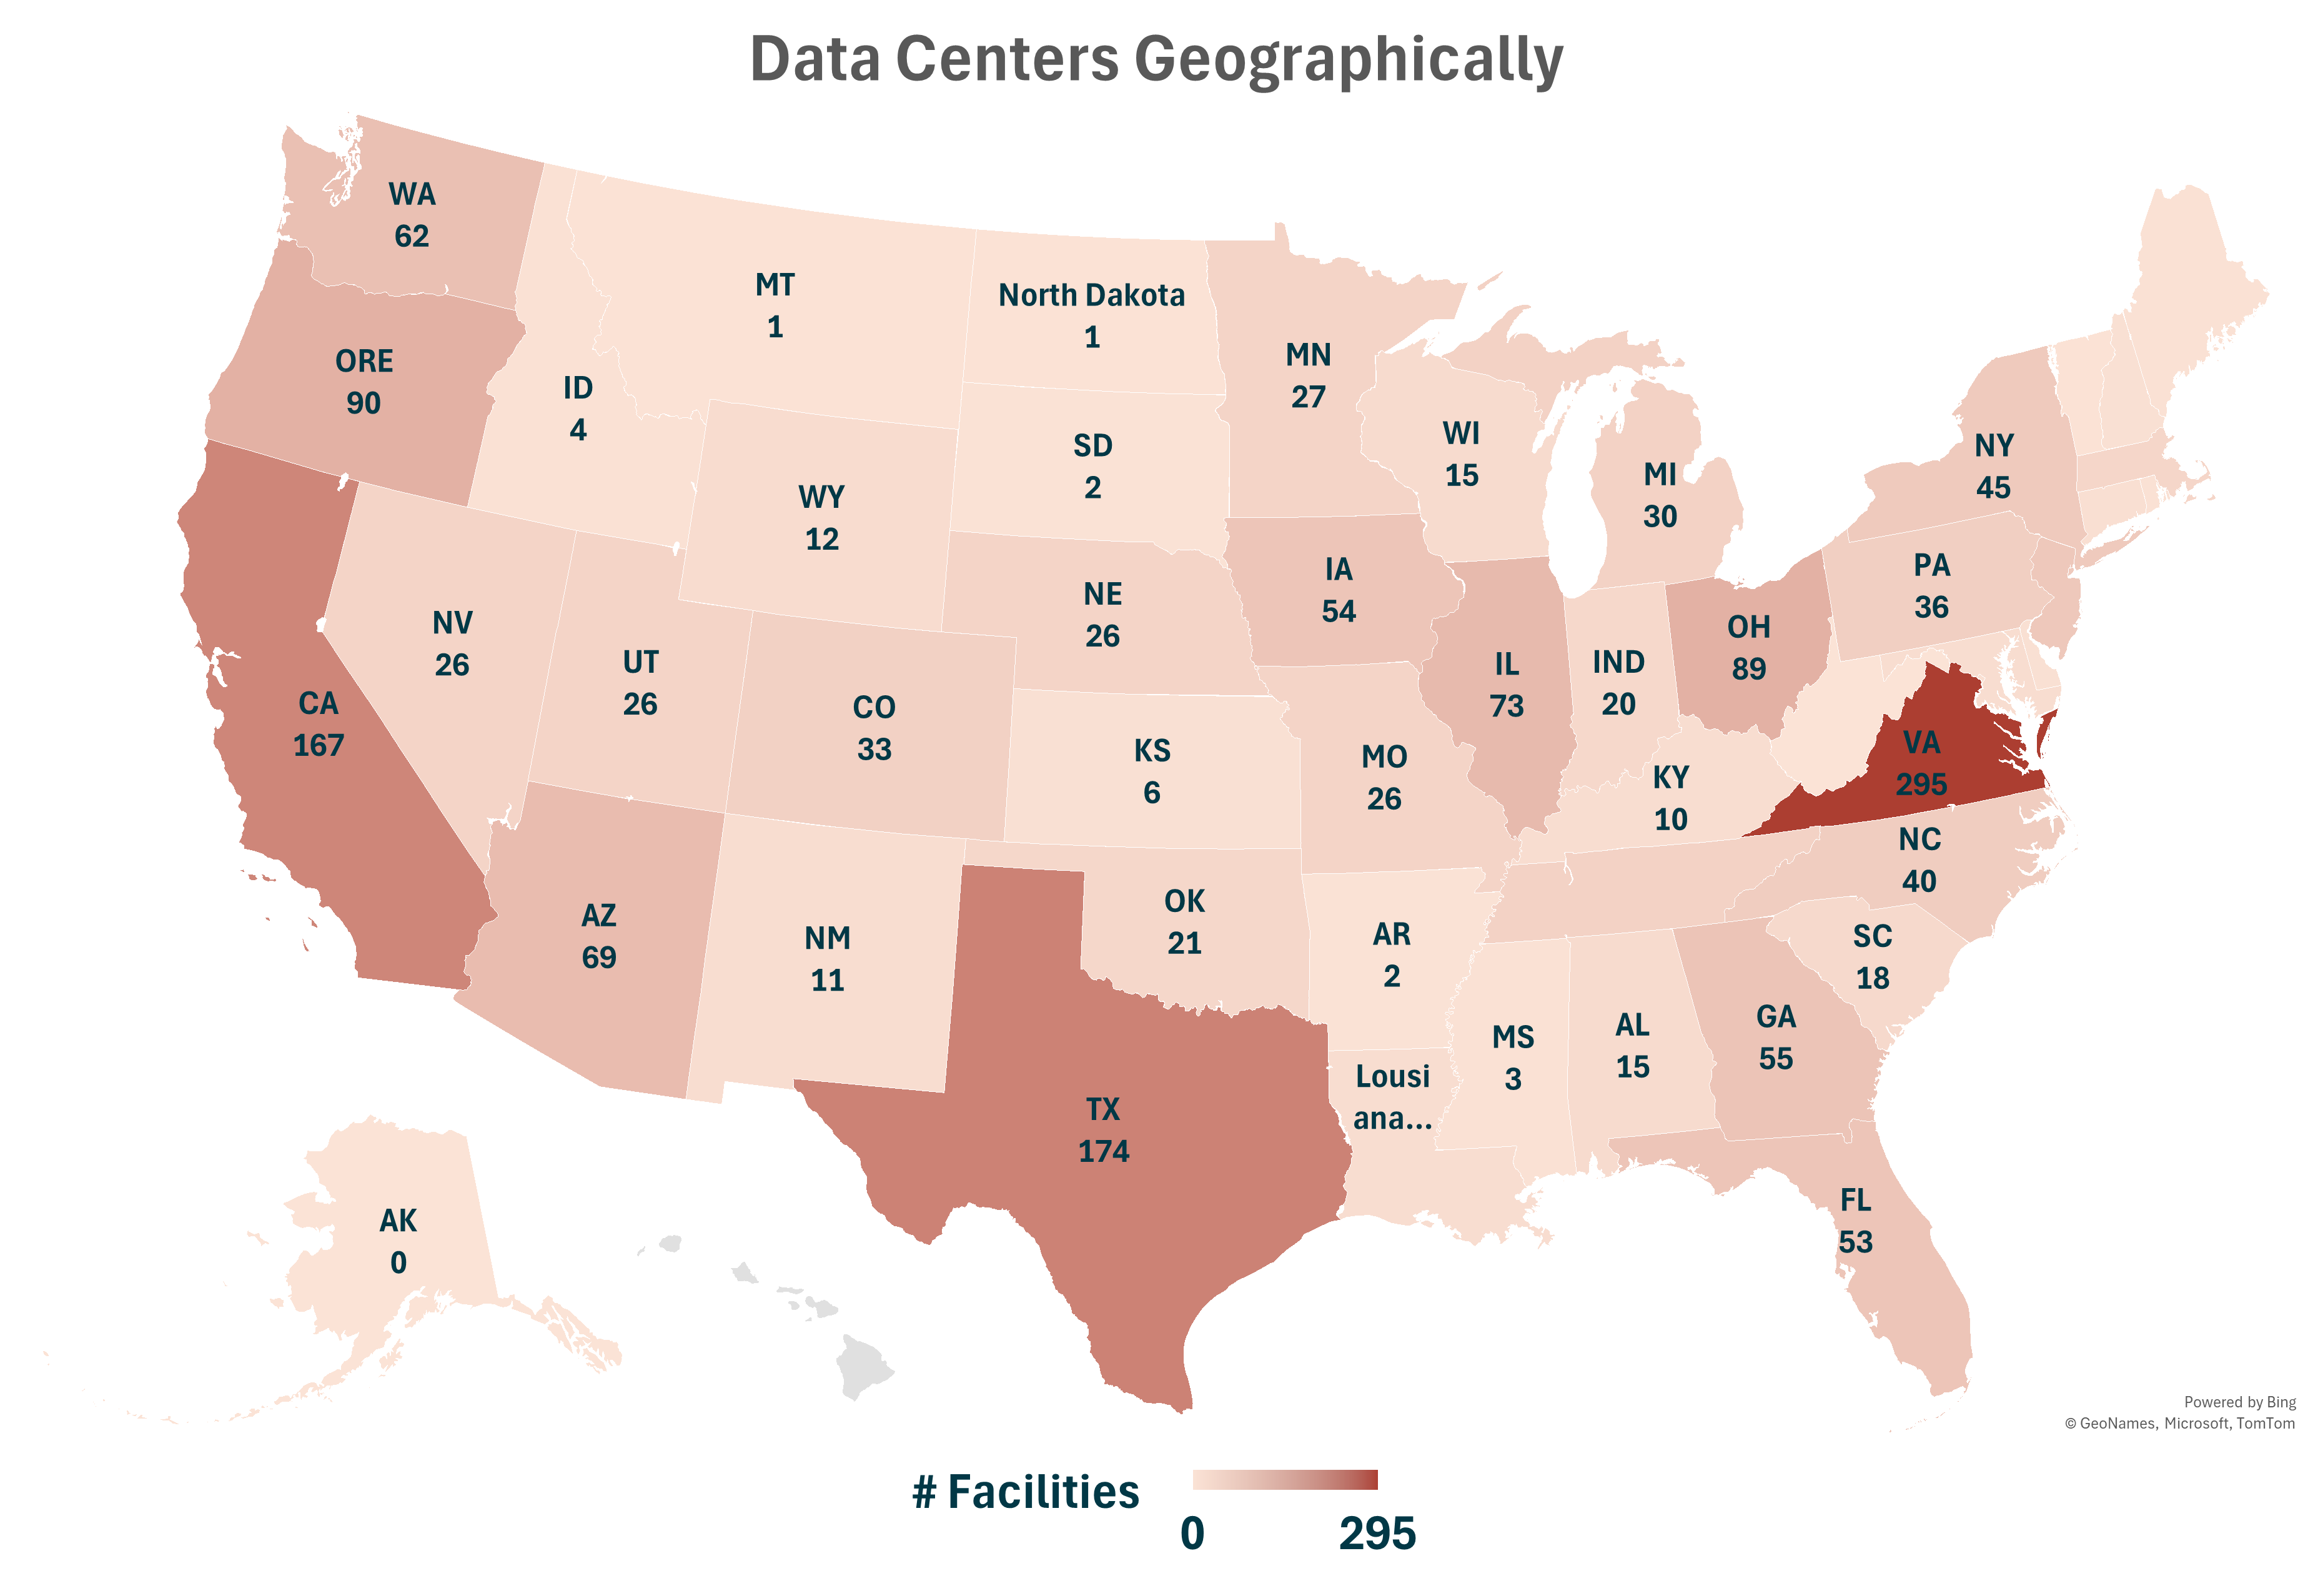
\includegraphics[width=\linewidth]{Figures/Data Centers by State.png}
%         \caption{Data centers by state. Source: Aterio.io. \niranjan{Dont think this picture contributes much to the discourse. Move to appendix for space.}}
%         \label{fig:DCbyState}
%     \end{minipage}
%     \hfill
%     % Second figure
%     \begin{minipage}[t]{0.45\linewidth}
%         \centering
%         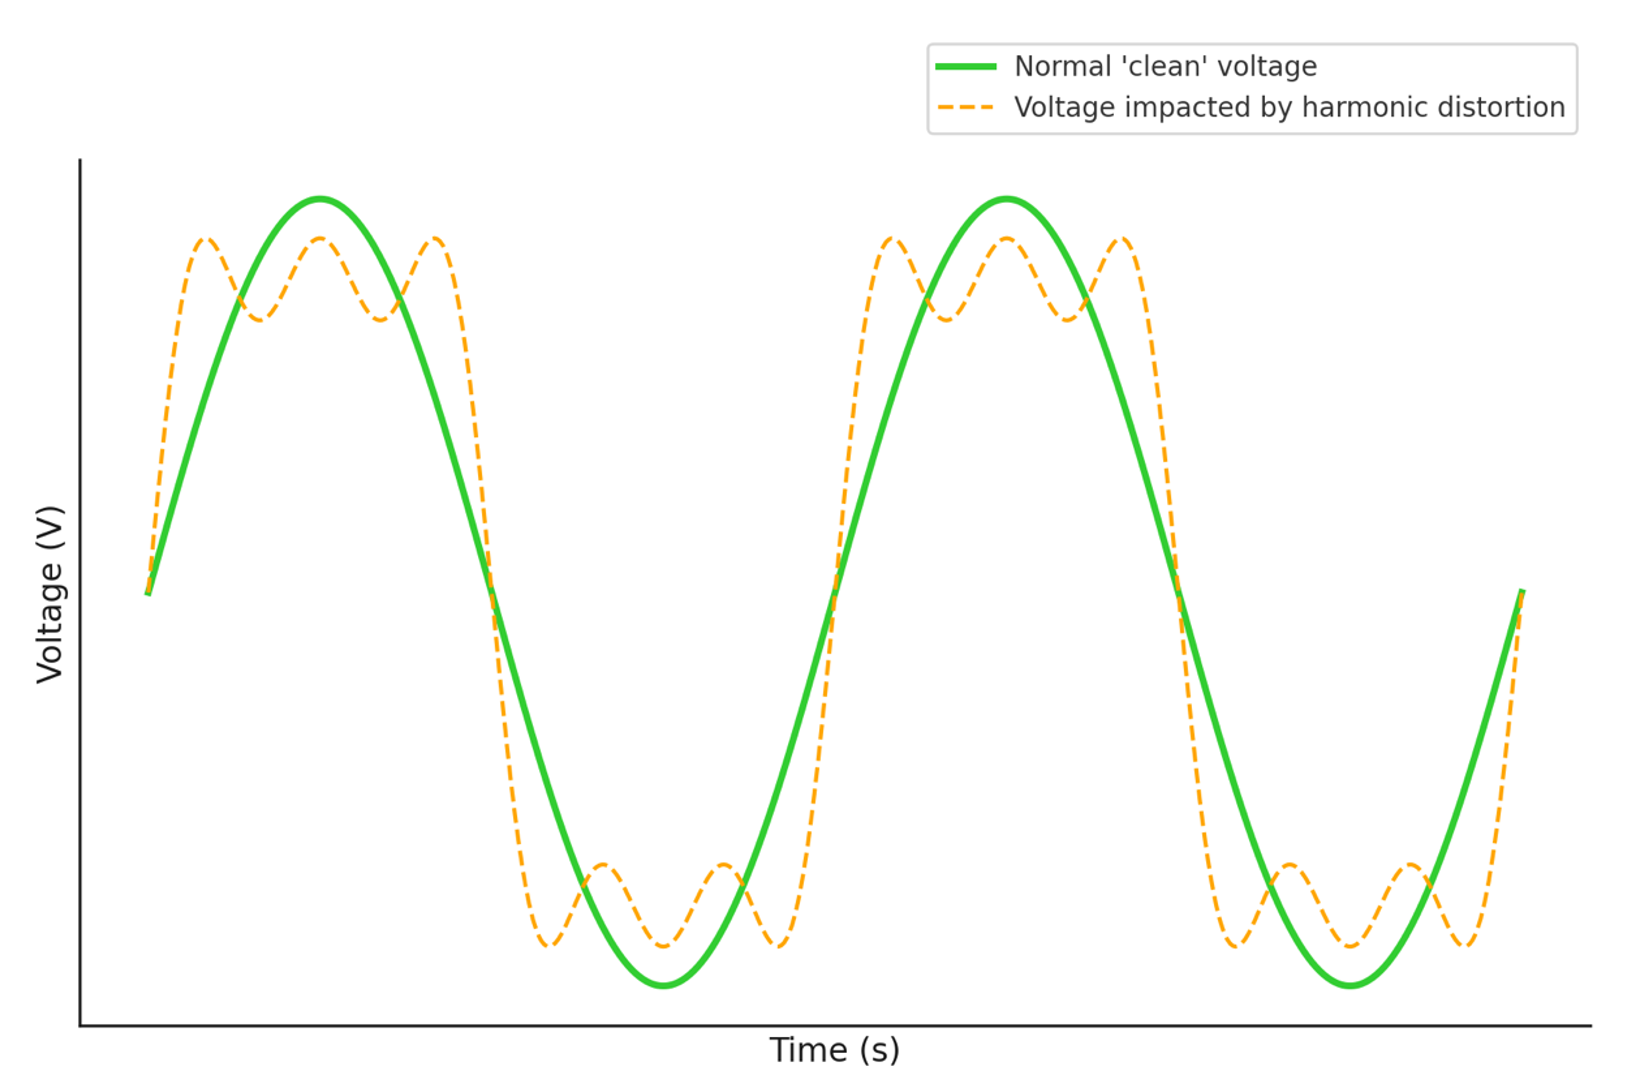
\includegraphics[width=\linewidth]{Figures/HarmonicDistortion.png}
%         \caption{Total harmonic distortion representation.}%\aruna{this figure is not referenced in the text}}        
%         \label{fig:THD}
%     \end{minipage}
%     \vspace{-2.05em}
% \end{figure}

% These economies of scale, however, generate externalities. Concentrated demand in specific regions strains local grids, raising congestion costs and sometimes degrading power quality for neighboring consumers. Large, inflexible loads reduce system reliability, elevate wholesale prices, and complicate renewable integration. At the same time, clustering provides local benefits through jobs, tax revenues, and downstream services. Data centers thus act as both efficiency drivers and sources of regional externalities. It is important to consider the mitigation of the externalities to the grid when analyzing the impacts of AI. We focus on hyperscalers in our paper because hyperscalers perform the majority of AI training and also because larger facilities are more likely to cause power distortions.
%\aruna{Is there a reason why we are talking about hyperscalers? Should we say therefore we focus on these hyperscalers?}



% The industry is also geographically concentrated. Texas, California, and especially Virginia dominate U.S. capacity. Virginia’s cluster reflects historic federal investments in internet infrastructure and the routing of early traffic through Northern Virginia. More recent growth in Texas stems from lower electricity costs and streamlined permitting.

% The electricity market includes three separate components: generation, transmission, and distribution. Generation is how power is produced. Transmission involves long-range transportation of electricity while distribution involves local distribution of electricity. In the United States, there are two primary models of how the electricity market is structured: vertically integrated utilities and deregulated markets. In vertically integrated utilities, which are prevalent in the South and West, generation, distribution, and transmission are all owned and operated by one company whereas in deregulated markets generation bids in wholesale markets to provide power to utilities, which own transmission and distribution, and provide power in the retail markets. Figure \ref{fig:ISOMap} provides a map showing the geographic makeup of the American electricity market.

% \begin{figure}
%     \centering
%     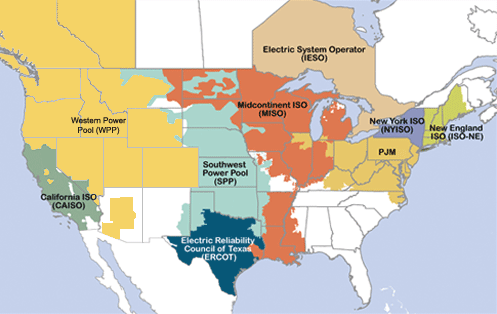
\includegraphics[width=0.5\linewidth]{Figures/ISOMap.png}
%     \caption{Map of American electricity market.}
%     \label{fig:ISOMap}
% \end{figure}

% These dynamics interact with broader shifts in the electricity market: greater electrification and the transition from fossil fuels to renewables. Because renewables are intermittent and less dispatchable, rising data center loads coupled with greater renewable penetration place dual pressures on grids, shaping both market outcomes and policy debates. It is therefore crucial to quantify how much power AI uses, how it distorts quality and impacts prices, and the role of efficiency improvements and developments in computing.
\section{Problem and Challenges}\label{Sec::Methods}

%\subsection{Problem}

% \nb{Compress to a single paragraph with the list of questions.}
% \nb{Note to self: some terminology can be expanded or replaced with more obvious descriptors (}
%\nb{The first three paragraphs can go away in the interest of space or be greatly compressed.}
%The U.S. data centers are expanding rapidly, nearly tripling from its 2008 levels to 1489 active sites in 2025, with another 1,359 on the horizon~\cite{aterio_us_data_centers_2025}. The market is dominated by \emph{hyperscalers}---vertically integrated datacenters---owned by AI heavy companies such as Amazon, Microsoft, and Google, alongside a long tail of smaller operators. 

%Hyperscalers afford companies certain economies of scale but greatly increase the geographic concentration of power demand on the grids. Concentrated demand strains local grids in the area, raising congestion costs and sometimes degrading power quality for neighboring consumers. Large, inflexible loads from AI hyperscalers also reduce system reliability, elevate wholesale prices, and complicate renewable integration.

%These dynamics interact with broader shifts in the electricity market: greater electrification and the transition from fossil fuels to renewables. Because renewables are intermittent and less dispatchable, rising data center loads coupled with greater renewable penetration place dual pressures on grids, shaping both market outcomes and policy debates. It is therefore crucial to quantify how much power AI uses, how it distorts quality and impacts prices, and the role of efficiency improvements and developments in computing.

Our goal is to investigate three primary effects of AI data centers on power markets. We also conduct counterfactual analyses that could inform policy: assessing different scenarios of parameter size, training versus inference proportions, edge compute preference, relocation to low-population areas etc.

\subsection{Problem introduced by AI workloads }

%First, we quantify whether the deployment of frontier AI models—which require extraordinary computational resources—coincides with measurable declines in regional power quality indices and frequency distortions near data centers. 

First, we quantify the effect of frontier AI models on power quality. % the deployment of frontier AI models—which require extraordinary computational resources—coincides with measurable declines in regional power quality indices and frequency distortions near data centers. 
AI workloads affect power quality through three main mechanisms. First, data centers and AI computing facilities add substantial baseload demand that can strain grid capacity and compromise voltage regulation, especially during peak periods. Second, AI workloads fluctuate rapidly with computational needs, creating unpredictable load variations that challenge stability and frequency regulation. Third, the switching power supplies and electronics essential to AI hardware generate harmonic distortion, introducing waveform distortions that spread through distribution networks and degrade power quality. See Figure \ref{fig:THD} in Appendix for an illustration of this harmonic distortion.



Second, we analyze how training and inference workloads differentially affect local power demand given that training produces sharp, episodic spikes while inference generates steadier ongoing consumption. 

Third, we estimate how wholesale electricity prices have responded to LLM development. % using price elasticities and treatment effects to approximate demand sensitivity and geographic price differentials across zones. %Finally, we conduct counterfactual analyses that could inform policy: assessing different scenarios of parameter size, training versus inference proportions, edge compute preference, relocation to low-population areas etc.
AI workloads  affect wholesale electricity prices through the demand channel, with potentially indeterminate long-run retail market impacts. %The U.S. electricity sector comprises both vertically integrated utilities and restructured markets featuring competitive wholesale generation alongside monopoly retail distribution. 
Wholesale prices are determined hourly in day-ahead markets via sealed-bid, uniform-price auctions subject to network constraints. Locational price variation reflects transmission limitations within the network. Increased demand raises wholesale prices by necessitating dispatch of higher-cost marginal generators. The wholesale price increases are passed through to retail consumers with substantial lag. Understanding wholesale demand and price shifts thus provides useful intuition regarding the direction and magnitude of retail price changes.

%\aruna{I commented some stuff out, take a look} DG: I think your comments look good (smile :)
%Retail rates typically reflect average procurement and distribution costs plus a state-regulated return on investment, calculated from historical data. This passthrough mechanism is indirect even absent investment-related dynamics. While new demand sources could theoretically dilute system-wide fixed costs and reduce average retail prices, increased demand more likely raises retail rates. Understanding wholesale demand and price shifts thus provides useful intuition regarding the direction and magnitude of retail price changes.


%we relate model parameter counts to grid impacts and how this relationship has evolved; estimate how AI efficiency gains could reduce power quality and demand effects; compare scenarios where AI compute is dominated by training versus inference; and evaluate geographic redistribution of compute—from cloud concentration to edge computing near population centers, or relocation to low-population areas with greater supply capacity. We also assess behind-the-meter generation as a potential grid relief mechanism.

%The main challenge in answering these questions is that the key variables of interest are not directly observable, either because they are proprietary or are prohibitively expensive. To address this we can use Difference-in-Differences, an econometric model that allows us to make causal inferences about impacts of model training and inference, even when direct observation is not feasible. However, applying this method is not without difficulties. First, the direct application of this idea requires that we know the exact start times for training and release dates for inference. Further, release dates can often be staggered. Last, the idea fundamentally relies on a \textit{parallel trends} assumption and robustness to confounds; we need to test if this assumption actually holds in our setting and check for other factors of influence. 

%The rest of this section lays out our methodology as follows: \autoref{EconometricModel} describes the econometric analysis model, presents the assumptions and the types of evidence needed to validate its use. \autoref{subsec:eventstudy} lays out the specific Event-Study design framework we use to address the staggered nature of our problem, and present its application for power quality, harmonic distortions, and fossil demand. \autoref{PriceEffects} presents our method for inferring price effects from power demand shifts.  \autoref{subsec:robustness} presents how we validate the use of the econometric models above. 

%Throughout the methods section, we describe the details of the econometric analysis, present assumptions and evidence that defend our choice to make them, and lay out the counterfactual analyses that will provide the key policy relevance of the paper. The section proceeds as follows. Subsection \ref{EconometricModel} describes the underlying logic behind the DiD econometric modelling techinque. Succeeding is Subsection \ref{subsec:eventstudy} where we detail the specific framework for the analysis of power quality, harmonic distortions, and fossil demand. We provide details on the event-study framework as a way to handle inability to see exact treatment periods. We continue with a discussion of how we identify data centers and link models to data centers in \ref{subsec:treatment}. We provide descriptions of the formal evidence we have demonstrating experimental validity and robustness in Subsection \ref{subsec:robustness}. This is directly anteceded by a description of the rationale between the difference between the power demand and power quality analysis in subsection \ref{subsec:differences}. We give insight into the estimation of price effects in Subsection \ref{PriceEffects}. We complete our tour of econometric methodology in the data center energy space with a look at our counterfactuals using evidence from previous results in Subsection \ref{counterfactuals} and a short digression about data center assumptions in Subsection \ref{DCASSUmptions}. 

% We analyze four primary effects of artificial intelligence (AI) data centers on the power market, with a focus on how their presence and operations interact with grid stability and demand.

% First, we consider the effects of AI models on the index of power quality and power frequency distortions in the vicinity of data centers. Power quality reflects the stability and reliability of the grid, particularly in terms of voltage and frequency deviations. The intensive and often irregular power draw of data centers—especially during periods of large-scale training runs—can generate fluctuations that degrade local power quality. Frequency stability is a central component of reliable electricity supply, and distortions can indicate imbalances between supply and demand. Because AI training loads are highly concentrated in time and location, they may create stress points in the grid that elevate the risk of such distortions. 
 
%  To this end, we evaluate whether the deployment of new frontier models, which require extraordinary computational resources, coincides with measurable declines in regional power quality indices, thereby signaling potential challenges for grid operators. Similarly, by linking model release timelines to observed patterns in frequency deviations, we assess the extent to which the roll-out of individual models exacerbates local power quality issues beyond baseline fluctuations.

% Second, we consider the effects of both training and inference workloads on overall power demand in the vicinity of data centers. Training runs, while episodic, are energy-intensive and can produce sharp spikes in consumption, whereas inference tends to generate a steadier but still substantial level of ongoing demand. Both activities alter local load profiles, raising questions about the adequacy of transmission capacity, the role of long-term contracts for renewable energy procurement, and the broader implications for regional electricity markets. By distinguishing between training and inference, we highlight how different stages of the AI lifecycle place unique and evolving pressures on power systems.

% Third, we analyze how wholesale electricity prices have been impacted by the development of LLMs. While we are unable to perform structural price analysis of LMP formation, we are able to use estimated price elasticities from our regressions alongside treatment effects to provide a ballpark estimate of the sensitivity of price to shifts in demand at the zonal level and how demand specifically from AI has contributed to differential price changes geographically across regions. We provide preliminary intuition on whether these wholesale price impacts have been transferred to the retail market to date and how these wholesale effects may in the future impact the retail market.

% Finally, we perform counterfactuals to inform stakeholders and policymakers about the potential impacts of differential evolution of LLM training, inference, and compute for AI at scale. We utilize data on parameter counts and specific features of AI models combined with our econometric estimates to provide evidence on the relationship between model size and grid impacts and how this relationship has changed over time. We then provide a back-of-the-envelope calculation relating AI efficiency to meaningful improvements in effects on power quality and demand. AI efficiency represents the main lever computer scientists have at their disposal to reduce the power consumption of AI models. 

% We further use our estimates to examine how AI impacts would differ in a world dominated by training with inference being less costly and mostly done on local devices and a world dominated by inference where training levels off as models plateau. We also utilize our econometric estimates to examine system level impacts of shifting compute geographically. We consider first a shift from cloud to edge computing wherein inference moves from concentration within hyperscalers to distributed inference closer to population centers. We contrast with a scenario where training and inference both move to low population areas with less load and more electricity supply better equipped to handle the influx of power demand. Finally, we analyze the role of behind-the-meter power generation as a potential alleviant to the grid. Together, our counterfactuals provide insight into how changes in the industry will shape the future of grid impacts and potentially directions the AI industry and policymakers could pursue to make impacts less palpable.
\subsection{An Econometric Model}\label{EconometricModel}
% \nb{change example to power quality}

%The main challenge in answering these questions is that the key variables of interest are not directly observable, either because they are proprietary or are prohibitively expensive. To address this we can use Difference-in-Differences, an econometric model that allows us to make causal inferences about impacts of model training and inference, even when direct observation is not feasible.

We want to quantify the effects of running AI models on the power grid but we only have overall observational data about power demand, power quality, prices, exogenous controls, locations of data centers, and dates of model activity. We do not have access to data that specifically isolates the effects with respect to running the AI models because these require proprietary knowledge. 

To address this challenge, we can turn to Difference-in-differences (DiD), a widely-used statistical estimation technique in econometrics for causal inference with observational data. This approach has been used to answer a wide range of empirical economics questions from observational data such as telecom demand from price and quantity variation, \citet{fowlie2012industrial} evaluate environmental regulation in electricity using emissions and price data, and \citet{card1994minimum} study minimum wage effects via cross-state employment variation.

%To directly quantify the effects of training or running a specific AI model on the power grid requires access to highly specific data. 
%Quantifying these effects is difficult given limited data on key variables. To overcome this, we draw on econometric methods, which allow credible inference even when proprietary data are unavailable. %We utilize the publicly announced dates of training and release as exogenous shocks. 
%\begin{wrapfigure}{r}{0.45\linewidth}
    
    %\vspace{-10pt} % adjust vertical position relative to the text
\begin{figure}            
    \centering
    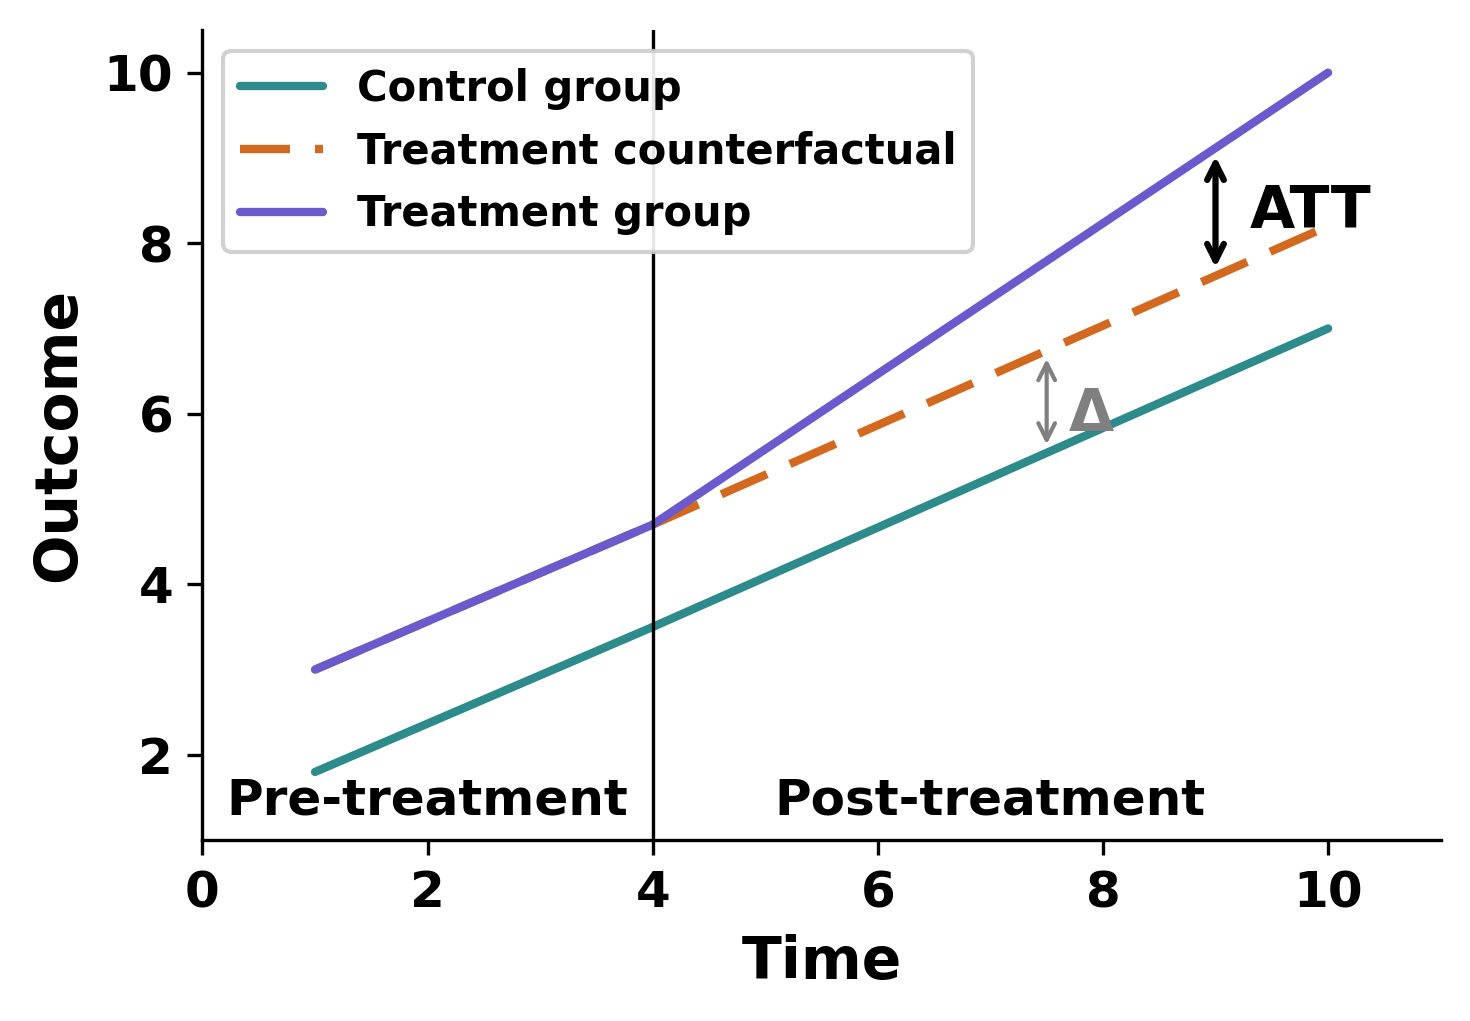
\includegraphics[width=0.6\linewidth]{Figures/did_estimation.png}
    \caption{Difference-in-differences estimation. Under the parallel trends assumption, the counterfactual (dashed) projects treatment group outcomes absent intervention. The ATT is identified as the divergence between observed and counterfactual outcomes post-treatment.}
    \label{fig:DIDFigure}
    \vspace{-2em}
\end{figure}
%\nb{Dana this figure can be redrawn to take up less vertically if you need space.}
%\nb{Expand the caption to describe what the plot shows at least cursorily.}
    %\vspace{-10pt} % tighten space below caption
%\end{wrapfigure}

%For example, \citet{hausman1997valuation} infers telecom demand from price and quantity variation, \citet{fowlie2012industrial} evaluate environmental regulation in electricity using emissions and price data, and \citet{card1994minimum} study minimum wage effects via cross-state employment variation. Similarly, \citet{greenstone2014environmental} analyze Indian pollution policy using ambient monitors rather than industry disclosures. These show that when markets transmit the mechanisms of interest, public data can yield the only feasible evidence. Our study follows this tradition: by exploiting observable shifts in prices, load, and capacity, we infer data center impacts that would otherwise remain opaque.

%\niranjan{Can we make this a more forceful paragraph by showing other solid papers that use this type of methodology? The following paragraph shows one paper, but lets add use cases where this is the only feasible approach.}
%The particular econometric tool we use to analyze the impacts of specific AI models is \textit{Difference-in-Differences} (DiD). Originally popularized in empirical economics through applications such as \cite{card2022design} on training programs and \cite{card1994comment} on minimum wages, difference-in-differences has become one of the most widely used methods for causal inference with observational data. 

The key idea behind this technique is to estimate treatment effects by comparing the change in outcomes over time for a treated group to the change for a control group, as illustrated in Figure~\ref{fig:DIDFigure}. 

For power quality, as an example, this translates to estimating the change in utility-level power quality within the geographically-defined utility area before and after the release of a major AI model. The treated group in this case would be utility areas containing data centers engaged in model training or inference during the time period of activity, and the control group would be utilities without AI activity in the same time period. The outcome variable, power quality in our example, is modeled as a function of the treatment (i.e. the running of the AI model), and other contributing factors. Formally, we can specify the power quality effect as:
\begin{equation}
    Y_{it} = \alpha + \beta \,(\text{Treatment}_i \times \text{Post}_t) + \gamma_i + \delta_t + \varepsilon_{it},
    \label{eq:DiD}
\end{equation}
where $Y_{it}$ is power quality for utility $i$ at time $t$, $\text{Treatment}_i$ indicates proximity to a data center, and $\text{Post}_t$ captures periods after the release of a major AI model. The coefficient of interest, $\beta$, measures the causal impact of model releases on local power quality. $\gamma_i$ captures unobserved factors common across all utilities, $\delta_t$ captures unobserved factors that remain fixed across time, and $\varepsilon_{it}$ is an error term that captures random disturbances or shocks. 

We can learn the co-efficients, given appropriate data about the outcome variables over time --- in this case with data about the power-quality values over time across a range of utilities containing AI data centers, and the knowledge of when and where the AI models of interest are run.
%By differencing across both groups and periods, DiD controls for unobserved factors that are constant over time or shared across groups, with validity relying on the ``parallel trends'' assumption. The data learns the coefficient of interest by taking the difference between the average change from the initial baseline between treated and untreated regions. 



\subsection{Technical Challenges and Validating Model Assumptions}\label{DCASSUmptions}
The validity of this basic DiD approach for our problem is affected by the following issues:
\begin{enumerate}
    \item \textit{Lack of specific information about when and where models are trained and released} The model as described requires knowing specifics of the training windows, e.g., when training began, and when it was released. It is not always possible to obtain such specific information. 
    \item \textit{Staggered Events} The model also assumes a single temporal event of interest to capture pre and post treatment effects. However, models are not always released at a single time point and are often staggered.    
    \item \textit{Parallel Trends Assumption} The effects of running a model on an AI data center is estimated by the difference from what would have been in the model were not run on that data center. This assumes that we have a fair estimate of the trend that the variable of interest would have over time but for the training and inference of the AI models. 
   
    \item \textit{External Confounds} The effects we observe and attribute to AI models could be due to other confounds such as random weather events, pre-existing trends in load, or variation in fuel price.
    \item \textit{Data Engineering Challenge} No single clean dataset contains all variables needed for analysis. Data often exist at different scales, lack linking tables, or require substantial preprocessing—sometimes necessitating manual mapping, combination, and labeling. An example is the zonal mapping effort used to assign generators to zones with the zonal map shown in Figure \ref{fig:MapofZonesRegular} in the Appendix.
    %\item \textit{Data Disparity and Relevance} Not all available observational data may be relevant to the treatment groups in our context. For example, \nb{Dana write an example here?}. 
    %\nb{write a few.} \nb{Also not sure if this is relvant}
\end{enumerate}
    
We address the first two challenges with a stacked modification of the DiD model (\autoref{subsec:eventstudy}). We address the next two through appropriate statistical tests and robustness checks (\autoref{subsec:robustness}) and the final issue through our data creation (section \ref{sectionData}). 

%\dana{Will add this to appendix. We could also add data center fixed effects.}
%\niranjan{This last point seems like }
%Finally, we directly state the limitations of our analysis and where the analysis could be improved with better data.

\section{Methodology} 

To address the inexact information about training windows and release times, we estimate dynamic treatment effects at multiple horizons relative to model release dates. This approach, referred to as an event study or \textbf{stacked difference-in-differences} in econometrics, offers three advantages over the standard pre/post comparison discussed earlier: (1) it does not require observing the true training start date, instead using release timing as the anchor; (2) it also provides a direct test of the parallel trends assumption through examination of pre-release coefficients; and (3) it allows the data to reveal the temporal profile of effects rather than imposing an arbitrary discontinuous treatment structure.

\subsection{Stacked DiD with Multiple Horizons}%Event-Study Framework}
\label{subsec:eventstudy}
Formally, we define treatment exposure relative to each model's release date $r_m$ for both training and release: \textbf{1) Training windows:} The period $[r_m - \bar{\tau}_{\text{train}}, r_m)$ preceding release, during which computational resources are devoted to model training. We remain agnostic about the exact training start date; our identifying assumption is that training activity is elevated in the months before release and that any pre-existing differential trends would manifest in the earlier leads. \textbf{2) Inference window:} The period $[r_m, r_m + \bar{\tau}_{\text{infer}}]$ following release, during which the model is deployed for inference via API access or public availability.


\subsubsection{Stacked Difference-in-Difference}

Model releases occur at different calendar dates, creating a staggered adoption setting. Recent econometric literature has demonstrated that conventional two-way fixed effects (TWFE) estimators as is the case in the estimates from Equation \ref{eq:DiD}. 
%\nb{is this referring to the standard DiD estimtor we have in Eq 1?} 
can produce biased estimates under treatment effect heterogeneity 
%\nb{don't know what treatment effect heterogenity means} in staggered designs 
\cite{goodman2021difference, sun2021treatment, callaway2021difference, borusyak2024revisiting}. Treatment effect heterogeneity means the policy works differently for different places or periods, which can distort standard difference-in-differences estimates. The bias arises because TWFE implicitly uses already-treated units as controls for later-treated units, and differences in treatment effects across cohorts or over time contaminate the estimated average. 

In our setting, consider regions as units and AI model releases as treatments inducing increased data center power demand. A "cohort" comprises regions whose data centers began significant AI workloads at the same time. Suppose Region A adopted AI workloads in 2022 while Region B adopted in 2023. When estimating treatment effects for Region B, TWFE implicitly uses Region A as a control—but Region A in 2023 is not untreated; its data centers have been running AI workloads for a year. If treatment effects evolve over time (e.g., power demand grows as AI infrastructure scales), comparing Region B's outcomes against Region A's already-treated outcomes introduces bias. Staggered design provides heterogeneity-robust estimators that solve for this exact issue.

%\nb{Can you explain the previous sentence in terms of data centers and time wrt power demand? It is hard to know what already-treated, later-treated units, cohorts etc mean.}

%We implement two complementary approaches to address this concern:
To address this, we use a stacked DiD model~\cite{cengiz2019effect, deshpande2019screened}, where we construct a stacked dataset where each model release defines a separate ``sub-experiment.'' The idea here is to construct, for each treatment cohort, a separate sub-experiment using only units that are genuinely untreated at the time of that cohort's adoption. By stacking these sub-experiments—each with its own clean control group of not-yet-treated regions—we ensure that no already-treated unit ever serves as a control, thereby eliminating the bias that arises when treatment effects are heterogeneous across cohorts or time.
%\nb{Dana, can you add a line that explains the idea and how it addresses the issue above}\nb{The idea here is to ....}

Formally, for each release event $m$, we create a dataset containing: (i) Treated units -- Regions linked to the releasing company's AI data centers. (ii) Control units -- Regions with no AI data center exposure during the event window, or regions whose treatment occurs sufficiently far from event $m$ that they serve as clean controls.
\begin{itemize}
    \item Time window: A symmetric window around $r_m$, e.g., $[r_m - K, r_m + K]$ for some horizon $K$.
\end{itemize}

Following \, we then stack these sub-experiments and estimate:
\begin{equation}
Y_{i,t,m} = \sum_{k=-K}^{K} \beta_k \cdot D_{ut}^k  + \delta_t + \mathbf{X}_{ut}'\theta + \varepsilon_{ut}
\label{eq:stacked}
\end{equation}
where $\gamma_{u}$ are unit-by-event fixed effects, $\delta_{u}$ are time-by-event fixed effects, $\mathbf{X}_{ut}'\theta$ represents controls, and the coefficients $\{\beta_k\}$ trace out the dynamic treatment effect at each event-time horizon $k$. Standard errors are clustered at the unit level to account for correlation across events within the same region.


\subsection{Estimating Power Quality}

Our power quality analysis estimates the following stacked DiD specification at the utility-month level:
\begin{equation}
\text{PowerQuality}_{ut} = \sum_{k=-K}^{K} \beta_k^{PQ} \cdot D_{ut}^k + \gamma_u + \delta_t + \mathbf{X}_{ut}'\theta + \varepsilon_{ut}
\label{eq:pq_eventstudy}
\end{equation}
where:
\begin{itemize}
    \item $\text{PowerQuality}_{ut}$ is the Whisker Labs Consumer Power Quality Index for utility $u$ in month $t$;
    \item $D_{ut}^k = \mathbf{1}[\text{event-time} = k] \times \text{Treated}_u$ indicates that utility $u$ is $k$ periods from the release date of a model linked to an AI data center in its service territory;
    \item $\gamma_u$ are utility fixed effects absorbing time-invariant characteristics;
    \item $\delta_t$ are calendar month fixed effects absorbing common temporal shocks;
    \item $\mathbf{X}_{ut}$ includes time-varying controls (weather, regional load).
\end{itemize}

We estimate an analogous specification for total harmonic distortion (THD):
\begin{equation}
\text{THD}_{ut} = \sum_{k=-K}^{K} \beta_k^{THD} \cdot D_{ut}^k + \gamma_u + \delta_t + \mathbf{X}_{ut}'\theta + \varepsilon_{ut}
\label{eq:thd_eventstudy}
\end{equation}

% \paragraph{Identifying Assumption.} \nb{Arent we moving this to 3.5 or 3.6?} The key identifying assumption is that, absent the AI model release, treated and control utilities would have followed parallel trends in power quality. We assess this assumption by examining the estimated coefficients $\{\beta_k : k < 0\}$ in the pre-release period. Under parallel trends, these coefficients should be statistically indistinguishable from zero. Systematic pre-trends would indicate either (a) anticipatory effects, (b) confounding from correlated unobservables, or (c) differential trends predating treatment.

\subsection{Estimating Fossil Fuel Demand}

Power demand analysis proceeds at the generator-month level, exploiting finer geographic resolution. We maintain the stacked DiD structure while incorporating instrumental variables to address the price endogeneity concern. Price endogeneity arises because electricity prices and demand are simultaneously determined—high demand pushes prices up, while high prices suppress demand—making it impossible to identify the causal effect of price on consumption from their correlation alone.

Two-stage least squares resolves this by isolating variation in price that is plausibly exogenous: in the first stage, we predict prices using an instrument that affects prices but has no direct effect on demand; in the second stage, we regress demand on these predicted prices rather than observed prices, recovering an unbiased estimate of the price elasticity.

% Power demand analysis proceeds at the generator-month level, exploiting finer geographic resolution. We maintain the stacked DiD structure while incorporating instrumental variables to address the price endogeneity concern. 
%\nb{Dana I added some content below to more clearly (aspirational :)) explain the rationale and what this does. Can you please check and fix inaccuracies?}
%Certain efficiency properties of the generators affects the generated electricity price, which in turn affects its demand. Similarly, other external causes such as prices of alternate sources of fuel also affects fossil fuel demand. To isolate the demand due only to AI data centers, we first identify the effects due to these other variables (i.e. supply-side cost shifters), and then predict the remaining effects on the demand in a second stage.


\paragraph{First Stage.} We instrument for electricity prices using supply-side cost shifters:
\begin{equation}
p_{it} = \pi_0 + \pi_1 \text{HeatRate}_{it} + \pi_2 \text{GasPrice}_{t} + \gamma_i + \delta_t + \mathbf{X}_{it}'\pi_3 + \nu_{it}
\label{eq:firststage}
\end{equation}
where $\text{HeatRate}_{it}$ captures the thermal efficiency of generator $i$ and $\text{GasPrice}_t$ is the contemporaneous natural gas spot price. These instruments satisfy relevance (they are primary determinants of marginal generation costs) and exclusion (they affect demand only through their impact on prices, not through direct effects on AI workload scheduling or other consumption decisions).

\paragraph{Second Stage.} We estimate the stacked DiD specification using predicted prices:
\begin{equation}
\text{FossilDemand}_{it} = \sum_{k=-K}^{K} \beta_k^{FD} \cdot D_{it}^k + \eta \hat{p}_{it} + \gamma_i + \delta_t + \mathbf{X}_{it}'\theta + \varepsilon_{it}
\label{eq:demand_eventstudy}
\end{equation}
where $D_{it}^k$ indicates event-time relative to model releases linked to AI data centers in generator $i$'s service area.

The coefficients $\{\beta_k^{FD}\}$ capture the dynamic effect of AI activity on fossil fuel demand. Negative values of $k$ (pre-release) correspond to the training phase; positive values correspond to inference. The price coefficient $\eta$ controls for supply-driven price movements and provides a scaling factor for welfare calculations. 
%Difference between samples in our main analyses are highlighted in the Appendix in Subsection \ref{subsec:differences}.

%\niranjan{Mention how the data is used to learn/estimate the co-efficients.}
%\niranjan{Add an equation here and refer to it in the text above.}

% \end{figure}
% \subsection{Empirical Strategy Details}
% This section presents our identification strategy for estimating the causal effects of AI model development on electricity grid outcomes. We analyze two primary outcomes: (1) power quality degradation at the utility level, and (2) fossil fuel generation demand at the generator level. Our approach employs an event-study framework centered on AI model release dates, with distinct treatment windows corresponding to the training and inference phases of AI development. We address identification challenges arising from staggered treatment timing, data limitations in linking models to specific training locations, and potential violations of parallel trends.



\subsection{Estimating Price Effects}\label{PriceEffects}
% \nb{Dana, please read this paragraph for my revisions.} DG: Looks good, I think.
% \nb{Make this more explanatory for someone who knows almost nothing about supply/demand and their relationships.}
Beyond quantity effects, we estimate how AI-driven demand increases affect electricity prices. The key economic insight is that price impacts depend on supply flexibility. In other words, when generators can easily expand output, increases in demand (e.g. AI-driven demand) can be easily absorbed with minimal increases in price. When the demand suddenly spikes (i.e. a demand shock), the prices will increase sharply as well. This is characterized using \textit{supply elasticity} $\varepsilon^s$—the percentage change in quantity supplied per one percent price change—quantifies this responsiveness.

%The key economic insight is that price impacts depend on supply flexibility: when generators can easily expand output, demand increases are absorbed with minimal price changes, but when supply is constrained, demand shocks translate primarily into higher prices. The supply elasticity $\varepsilon^s$—the percentage change in quantity supplied per one percent price change—quantifies this responsiveness.

Our estimation proceeds in two steps. First, we use our IV estimates to quantify how AI activity shifts demand. Simply put, the average change in total fossil demand from AI demand is the DiD coefficient times the treatment indicator:
\begin{equation}
\Delta \widehat{\text{FossilDemand}}{it} = \hat{\beta} \cdot \Delta \text{AI}{it}
\label{eq:demand-change}
\end{equation}
% \nb{Dana, say what the RHS terms are. }
Second, we estimate a linear supply relationship using demand controls as instruments and supply shifters as controls. While power markets involve optimal dispatch, the fossil-fuel portion of PJM’s marginal cost curve is approximately linear over the operating range we study \cite{PJM_DataMiner2_2025}.
%\nb{Dana check the following paragraph.}
%Second, we trace this shift through the supply curve which encodes the relationship between the price and the supply that generators are able to provide.%\nb{We dont know what a supply curve is. Yes, we are completely ignorant!}. 
Let $p_i$ denote the market-clearing price in market $i$, and let $Q^s$ denote
the supplied quantity. We model supply locally as linear in price,
$Q^s = a + b \cdot p_i$, where the slope parameter $b$ captures the
responsiveness of supplied quantity to price changes (i.e., how flexibly
supply can adjust to incentives). Rearranging, the implied price response to a
demand shift $\Delta AI_{it}$ is given by
$\Delta p = \hat{\beta} \cdot \frac{\Delta AI_{it}}{b}$. Expressed in percentage
terms, the price impact depends on the flexibility of supply with respect to
price:
\begin{equation}
\% \Delta p = \frac{\% \Delta Q^d}{\varepsilon^s},
\label{eq:price-impact-elasticity}
\end{equation}
where $\varepsilon^s$ denotes the percentage change in supplied quantity per
percentage change in price.
%\nb{Say what $Q^s$, $p_i$ are. elasticity is not a term we know. Use a descriptive phrase also}

% \begin{equation}
% \% \Delta p = \frac{\% \Delta Q^d}{\varepsilon^s}
% \label{eq
% :price-impact-elasticity}
% \end{equation}

We estimate $\varepsilon^s$ via IV regression of quantity on price in log-log form, using demand-side instruments (weather-driven load variation and industrial production indices).

We focus on the PJM operator at the zonal level for this analysis. We restrict to a single ISO (operator) because differing market structures make prices incomparable across ISOs, and choose PJM because it is the largest (65 million people, 13 states), includes key data center states (Virginia, Pennsylvania), and provides 20 diverse pricing zones. Because observed training locations are outside PJM, this analysis uses the broader model set only.
% \paragraph{Demand Change from Treatment Effect.} The estimated coefficient $\hat{\beta}$ gives the predicted demand change for a given change in AI activity:
% \begin{equation}
% \Delta \widehat{\text{FossilDemand}}_{it} = \hat{\beta} \cdot \Delta \text{AI}_{it}
% \label{eq:demand-change}
% \end{equation}

% \paragraph{Price Impact via Supply Elasticity.} A demand shift $\Delta Q^d$ yields a price change determined by supply responsiveness. With linear supply $Q^s = a + b \cdot p$:
% \begin{equation}
% \Delta p = \frac{\hat{\beta} \cdot \Delta \text{AI}_{it}}{b}
% \label{eq:price-impact}
% \end{equation}
% In elasticity form, for a percentage demand increase $\% \Delta Q^d$:
% \begin{equation}
% \% \Delta p = \frac{\% \Delta Q^d}{\varepsilon^s}
% \label{eq:price-impact-elasticity}
% \end{equation}
% We estimate $\varepsilon^s$ via two-stage IV regression of quantity on price in log-log form, using demand-side instruments (weather-driven load variation and industrial production indices) rather than supply-side instruments. We then combine this elasticity estimate with the demand shift from earlier regressions to calculate price impact. For specifically this regression, we focus on the Independent System Operator (ISO) PJM at a zonal level. We choose to focus on one ISO because differently structured capacity markets and differing market structures mean that prices are not truly equivalent across ISOs. We focus specifically on PJM because it is the largest ISO by population including 65 million people over 13 states and crucially includes Virginia and Pennsylvania, two of the main data center hotbeds. PJM also has 20 diverse zones providing the neccecary granularity. Because the observed training locations are not in PJM, this analysis can only be conducted with the broader model set and not our conservative main analysis.
% \begin{center}
% \textit{[PLACEHOLDER: Table of models with verified training start dates, training end dates, and API/inference release dates from public announcements, papers, or regulatory filings]}
% \end{center}

\subsection{Validating Assumptions and Robustness}
\label{subsec:robustness}

We implement several diagnostic and robustness tests to assess the credibility of our estimates.

\subsubsection{Sample Selection}

Our empirical strategy balances internal validity with external relevance. Our main sample comprises four models for which we observe exact training and inference dates as well as training location, and we employ propensity score matching (described in the appendix) to support the parallel trends assumption. We then report results for progressively larger samples of models and data centers, accepting weaker identification in exchange for broader coverage. This approach enables precise, well-identified estimates from our core sample while exploring heterogeneity and counterfactuals in extended samples, with appropriate caveats regarding the latter.

% We vary our sample, so we can provide highly robust estimates of treatment effects using a sample we have exceptional information about while exploring observed heterogeneity in larger samples to enable interesting analysis and counterfactual. We demonstrate robustness for the samples that are less controlled. In our main sample, we focus on four models for which we know exact training and inference dates as well as the location of training. We also utilize propensity score matching as described in the appendix in order to ensure the satisfaction of the parallel trends assumption. We report results for alternative progressively larger samples of models and datacenter with fewer robustness protections to provide a fuller picture with the caveat that less confidence exists in the estimated results. We feel that this conservative approach both allows us to make specific and measured statements and also broader but more impactful statements.

\subsubsection{Pre-Trends and Parallel Trends Testing}

Our primary test of the identifying assumption examines whether pre-release coefficients $\{\beta_k : k < 0\}$ are jointly indistinguishable from zero. We report:
\begin{itemize}
    \item Point estimates and confidence intervals for each lead coefficient.
    \item An F-test of the joint null hypothesis $H_0: \beta_{-K} = \beta_{-K+1} = \cdots = \beta_{-1} = 0$.
\end{itemize}
Significant pre-trends would undermine the causal interpretation of post-release estimates.

\subsubsection{Placebo Tests with Randomized Treatment Assignment}

To verify that our estimates reflect genuine treatment effects rather than spurious correlations or specification artifacts, we conduct placebo tests with randomly assigned treatment:
\begin{enumerate}
    \item \textbf{Random treatment timing:} We hold the set of treated units fixed but randomly reassign release dates drawn from the empirical distribution of actual release dates. Under the null of no effect, placebo estimates should center on zero.
    \item \textbf{Random treatment assignment:} We hold release timing fixed but randomly reassign treatment status across units. This tests whether results are driven by the specific geographic pattern of AI data center locations.
\end{enumerate}
% For each placebo design, we generate five draws and compare our actual estimates to the distribution of placebo estimates. We report the share of placebo estimates exceeding our point estimate in absolute value (a randomization inference p-value).

% \nb{Dana, add some text that says how this relates to the paragraph above?}
\subsubsection{Sensitivity to Treatment Definition}

Given uncertainty in linking models to specific training locations, we assess robustness to alternative treatment definitions in our less conservative analysis:
\begin{enumerate}
    \item \textbf{Intensive margin:} Weight treatment by the number or capacity of AI data centers in the region, rather than using a binary indicator.
    \item \textbf{Dropping ambiguous cases:} Exclude model releases where the company operates data centers in multiple balancing authorities, restricting to cases with cleaner geographic attribution.
    \item \textbf{Verified timing subset:} Estimate separately on the subset of models with externally verified training windows.
    \item \textbf{Geographic Resolution and Robustness.} The generator-level data permit more granular treatment definitions than the utility-level power quality data. We exploit this flexibility by estimating specifications under alternative treatment definitions in terms of radius.
\end{enumerate}

\subsubsection{Heterogeneity by Model Characteristics}

We examine whether treatment effects vary with observable model characteristics:
\begin{itemize}
    \item Model scale (parameter count, reported compute).
    \item Company (to assess whether effects are driven by specific firms).
    \item Release year (to assess whether effects change over time).
\end{itemize}
Heterogeneity analysis both informs mechanisms and serves as a specification check: if effects are concentrated among larger models or models from companies with substantial AI infrastructure, this lends credibility to the AI-driven interpretation.

\subsection{Counterfactual Analysis}\label{counterfactuals}%Efficiency Impact Model}\niranjan{Compress}

We conduct three primary sets of counterfactual exercises to investigate how alternative evolutionary paths for AI compute might affect grid-level outcomes.
%Additional counterfactuals with results are highlighed in Appendix Subsection \ref{Appendix:Counterfactuals}.

\textbf{Model Scaling.} First, we examine the grid implications of continued growth in AI model size. Using the Epoch database to characterize trends in model parameters, we provide descriptive analysis of how increasing model scale translates into grid-level impacts. We then relate our estimated power demand coefficients to power quality coefficients, enabling analysis of how changes in training and inference energy efficiency propagate to power quality outcomes.

\textbf{Geographic Redistribution.} Second, we leverage the geographic locations of data centers in conjunction with our econometric estimates to conduct counterfactuals focused on spatial reallocation of AI compute. We consider two scenarios. In the first, we simulate a shift from cloud-based to edge-based inference—reallocating inference demand from concentrated hyperscaler facilities to smaller data centers distributed closer to population centers. We implement this by redistributing our estimated inference demand impacts across data centers not currently classified as AI-focused. In the second scenario, we simulate relocating training workloads from population-dense regions on the East Coast to energy-abundant regions in the center of the country. For both geographic counterfactuals, we provide sensitivity analyses in the appendix to account for potential increases in communication costs and efficiency losses.

\textbf{Colocated on-site Power Generation.} Finally, we exploit a new feature in the Aterio data, namely a flag on data centers with on-site power generation. We re-estimate both our main models separately for generators with and generators without onsite power generation. We then report the impacts to power demand and power quality of either removing all onsite generation or having onsite generation for all data centers.


Together, these counterfactuals illuminate both how the grid might be affected by different trajectories for AI compute and which levers—geographic placement, workload composition, efficiency improvements—may be available to computer scientists and policymakers seeking to mitigate grid impacts.
%\niranjan{The main idea is to design regressors that can tell us how changes in efficiency e.g., reduction in model parameters, impacts power quality and demand. Note we already have a model for how the power quality changes for a certain set of AI model releases. We can use this to .... To do this we need... }

%Our methodology combines econometric estimates with data from the Epoch database on the number of parameters of models as well as estimates of the impacts of increasing model parameters on relative energy usage. We perform regressions on our coefficients on training compute FLOPS and parameters. This allows us to determine how relative increases in the model's efficiency can lead to changes in model power demand and quality.

%We also perform a techno-economic analysis of the impacts of increasing model size and the number of simultaneous GPUs on energy consumption. This analysis combines econometric estimates with experimental evidence we generated by training a subset of smaller models under different GPU counts and sizes, allowing us to directly observe the contribution of message passing between GPUs to total training energy costs. We essentially extrapolate our experimental results to larger production-level models to estimate the real-world impact of the power reductions from the experiments. Together, these approaches provide a framework for translating trends in AI model scaling into counterfactual grid-level impacts.

% We also run a difference-in-difference regression of the entire length of the interconnection queue and the length of the interconnection queue specifically for natural gas for counties before and after the announcement of a major data center.

% \begin{equation*}
% \text{TotalQueue}_{ct} = \alpha' 
% + \beta' \left( \text{Post}_{t} \times \text{Treatment}_{c} \right)
% + \gamma'_c + \delta'_t + \varepsilon'_{ct}
% \end{equation*}

% \begin{equation*}
% \text{GasQueue}_{ct} = \alpha 
% + \beta \left( \text{Post}_{t} \times \text{Treatment}_{c} \right)
% + \gamma_c + \delta_t + \varepsilon_{ct}
% \end{equation*}

% We also interact the capacity and square footage of the data center with the variable for after the data center's implementation to determine the impact of a MW of capacity from data centers on the interconnection queue. This provides an understanding of how natural gas investments increase following data center announcements and provides evidence for how data centers impact capacity investments.

% \begin{equation*}
%     \text{GasQueue}_{ct} = \alpha + \beta_1 \left( \text{Post}_{t} \times \text{Capacity}_{c} \right)+ \gamma_c + \delta_t + \varepsilon_{ct}
% \end{equation*}

% \begin{equation*}
%     \text{GasQueue}_{ct} = \alpha + \beta_2 \left( \text{Post}_{t} \times \text{SqFt}_{c} \right)+ \gamma_c + \delta_t + \varepsilon_{ct}
% \end{equation*}

% In order to consider the impacts of PPAs by data centers, we look at EIA form 860 data on capacity investments in counties with data centers as well as counties with PPAs by tech companies. PPA data comes from S\& P Capital IQ Pro and is used to perform difference-in-differences regressions of entry capacity of renewable resources on power purchase agreements. We further perform a similar regression of capacity investments in natural gas on announcements of data centers to determine whether PPAs are leading to more renewable or fossil fuel capacity additions.

% % 1. Renewable capacity entry and PPAs
% \begin{equation}
% \text{RenewCap}_{ct} 
% = \alpha 
% + \beta \, (\text{PPA}_c \times \text{Post}_t) 
% + \gamma_c + \delta_t 
% + \varepsilon_{ct}
% \end{equation}

% % 2. Fossil (natural gas) capacity entry and data center announcements
% \begin{equation}
% \text{GasCap}_{ct} 
% = \alpha 
% + \theta \, (\text{DCAnnounce}_c \times \text{Post}_t) 
% + \gamma_c + \delta_t 
% + \varepsilon_{ct}
% \end{equation}

% \subsection{Controls}
% \aruna{Not clear if we need this section given we discuss the controls in each of the specific section, thoughts?}
% The difference-in-differences framework relies on the assumption that, absent treatment, outcomes for treated and control groups would have evolved along parallel trends. Potential threats to this assumption include \emph{group-specific shocks} such as local infrastructure upgrades or outages that disproportionately affect power quality, \emph{anticipation effects} including preemptive grid adjustments ahead of a model release, and \emph{spillovers} like load shifting from nearby control regions. Any of these could bias estimated treatment effects if not properly accounted for. To mitigate these risks, we incorporate controls for weather and fuel prices, as well as geographic and temporal fixed effects. For instance, we explicitly model the impacts of weather conditions by including weather control variables to ensure that systematic climatic variation—which could influence both electricity demand and grid stability—does not confound our estimates.


\section{Data}\label{sectionData}
%\niranjan{To address the three questions we need the following data -- refer to data about variables of interest, control data}
%\niranjan{What we have now is the data of this kind. Who publishes it ... We combine these sources to obtain this data.}
Table \ref{tab:DataSources} summarizes the datasets we use to address each of our three research questions, distinguishing between variables of interest and the control variables described above. For variables of interest, we rely on \textbf{Aterio}, which provides comprehensive information on the location and history of data centers. The Aterio dataset documents when and where centers have been established, expanded, or retired, along with details on ownership and operational capacity (in MW). This allows us to identify data centers owned by specific hyperscalers and to quantify their scale over time. We then combine these data with external sources that provide the necessary controls. 
%\nb{Dana, verify if the following is a correct characterization. If not please fix.} DG: Looks fine. My one thing is that maybe leave out GPT-4 as GPT-4 is only in our sample for power quality and THD and not demand.
The data centers we use include ones that we could verifiably trace as having been the source of training of well-known large scale models such as GPT-3, PaLM, and Llama 2, among others.
\begin{table}[t!]
\scriptsize % smaller font for compression
\centering
\caption{Data sources for each analysis question.}
\label{tab:DataSources}
\begin{threeparttable}
%\begin{tabularx}{\linewidth}{lXXl}
\setlength{\tabcolsep}{3pt} % tighter columns (optional)
\renewcommand{\arraystretch}{1.05} % slightly tighter rows (optional)
\begin{tabularx}{\linewidth}{>{\raggedright\arraybackslash}p{1.1cm} X X p{2.2cm}}
\toprule
\textbf{Source} & \textbf{Content} & \textbf{Use in Analysis} & \textbf{\# Instances} \\
\midrule
\multicolumn{4}{c}{\textbf{Q1: Difference-in-Differences (Power Quality)}} \\
\midrule
Aterio & Data center locations, history, ownership, capacity (MW) & Define treatment regions; link AI model releases & 3862 data centers\\
Whisker Labs & CPQI (consumer reliability); THD (waveform distortion) & Outcome variables for DiD regressions & 2684 utility-months\\
EIA & Retail service territory maps & Define treatment/control boundaries & 72 utilities\\
\midrule
\multicolumn{4}{c}{\textbf{Q2: Instrumental Variables (Fossil Demand)}} \\
\midrule
EPA CAMPD & Hourly generator demand; heat rates & Fossil demand outcome; heat rate as instrument & 22 million generator-hours\\
S\&P Capital IQ & Natural gas prices & Instrument and fuel-cost control &12 Million location-day prices \\
Aterio & Data center proximity to generators & Treatment near releasing-company centers & 3862 data centers\\
Meteostat & Temperature, precipitation & Demand and renewable controls & 22 million location-hours\\
ISOs & Zonal wholesale prices & Market controls & 54 zones\\
\midrule
\multicolumn{4}{c}{\textbf{Q3: Counterfactual Analyses (Technical Evolution of AI)}} \\
\midrule
Whisker Labs & CPQI; THD & Baseline power quality impacts for scaling projections & \\
Epoch & Model parameters, FLOPs, release dates & Scaling regressions; efficiency counterfactuals & 75 models\\
% GPU Experiments & Energy use with varying GPU counts/sizes & Extrapolate to production models & \\
\bottomrule
\end{tabularx}
\end{threeparttable}
\end{table}


%\niranjan{This following paragraph can be compressed since we detail the sources under 5.2 anyway. Just keep the first line and toss the rest. If there are additional pieces of information here then merge them into 5.1 and 5.2 as appropriate.}
 %Weather data come from \textbf{Meteostat}, which reports hourly temperature and precipitation; fuel cost data are obtained from \textbf{S\&P Capital IQ Global}, which publishes historical natural gas price series; and generator-level demand and heat rate data are published by the \textbf{EPA} through the Continuous Air Monitoring and Power Data (CAMPD). In addition, we construct zonal market boundaries using maps provided by \textbf{U.S. Independent System Operators (ISOs)} and merge these with ISO wholesale price data. Finally, we use geographic service territory files from the \textbf{EIA} to ensure consistent alignment of generator-, zonal-, and retail-level observations across datasets.  

\subsection{Data and Empirical Specification}
We analyze four primary outcomes. \textbf{The Consumer Power Quality Index (CPQI)} from \cite{WhiskerLabs_THD_2024} provides a composite measure of consumer-facing reliability events (surges, sags, brownouts, interruptions), summarizing frequency and severity of power deviations at the household level. \textbf{Total Harmonic Distortion (THD)} data from the same source offer a technical measure of waveform distortion, quantifying voltage deviation from a clean 60-Hz sine wave; elevated THD indicates grid stress, reduces motor efficiency, and shortens equipment lifespan (Figure \ref{fig:THD}). Since THD data are more recent than CPQI, fewer model releases are available for THD analysis. We incorporate \textbf{generator demand} from EPA's CAMPD database, providing hourly plant-level demand spanning 2021–2023. Finally, we combine \textbf{wholesale zonal price data} from Independent System Operators (ISOs) to assess AI impacts on prices.

Our power quality regressions use a parsimonious specification with time and geographic fixed effects. Generator demand regressions employ a richer specification: we instrument for endogeneity using generator heat rates and natural gas prices (S\&P Capital IQ Global) in a two-stage least squares framework, and control for weather conditions (Meteostat) to capture demand and renewable variability. EIA retail service territory files reconcile generator-, zonal-, and retail-level observations.
 % \subsection{Variables of Interest}
% %\niranjan{separately specify the variables of interest and the data needed for each question here. call them out explicitly with bold face or italics or some headings.}
% We use four primary datasets for our outcomes of interest. First, the \textbf{Consumer Power Quality Index (CPQI)} from \cite{WhiskerLabs_THD_2024} provides a composite measure of consumer-facing reliability events (surges, sags, brownouts, interruptions), summarizing frequency and severity of power deviations at the household level. Second, \textbf{Total Harmonic Distortion (THD)} data from \cite{WhiskerLabs_THD_2024} offers a \emph{technical measure of waveform distortion}, quantifying voltage deviation from a clean 60-Hz sine wave. Elevated THD indicates grid stress, reduces motor efficiency, and shortens equipment lifespan. Figure \ref{fig:THD} illustrates how harmonics alter voltage sine waves, reducing power reliability. Since THD data are more recent than CPQI, fewer model releases are available for THD analysis. Third, we incorporate \textbf{generator demand} from EPA's CAMPD database, providing \emph{hourly plant-level demand} that captures local operating characteristics. CAMPD data span 2021--2023, constraining analysis to AI model releases within that period. Finally, we combine \textbf{wholesale zonal price} data provided by Independent System Operators (ISOs) to determine AI impacts on price.
% \subsection{Control Variables}
% For the \textbf{power quality regressions}, we use a parsimonious specification with only time and geographic fixed effects, which absorb seasonal patterns, long-run trends, and location-specific differences, allowing us to test whether data center activity coincides with reliability declines beyond geography and time. In contrast, the \textbf{generator demand regressions} employ a richer set of controls to address endogeneity, using \emph{generator heat rates} from EPA CAMPD and \emph{natural gas prices} from S\&P Capital IQ Global as instruments in a two-stage least squares framework, along with CAMPD’s hourly generator demand data (2021–2024). We also incorporate \emph{Meteostat} weather variables (temperature, dewpoint, precipitation) to capture demand and renewable variability, and \emph{ISO} market data based on boundary maps to ensure spatial consistency. Finally, \emph{EIA retail service territory files} reconcile generator-, zonal-, and retail-level observations into a consistent framework.
% For the \textbf{power quality regressions}, we deliberately keep controls parsimonious. Because the areas for which power quality is measured are much larger and the available dataset is significantly smaller, we restrict the specification to time and geographic fixed effects. These absorb broad seasonal patterns, long-run trends, and location-specific differences that could confound observed changes in power quality. We do not include fuel or generator-level variables here, because the goal is to isolate whether data center activity coincides with localized deteriorations in reliability beyond what is explained by geography and time.  
% In contrast, for the \textbf{generator demand regressions}, we employ a richer set of external data sources to address the endogeneity of prices and generation. In particular, we use \emph{generator heat rates} from the EPA’s Continuous Air Monitoring and Power Data (CAMPD) and \emph{natural gas price series} from S\&P Capital IQ Global as instruments in a two-stage least squares framework. Heat rates capture technological efficiency at the unit level, while natural gas prices reflect exogenous shifts in input costs; both provide valid sources of variation to predict electricity prices without being directly affected by AI model releases. The CAMPD data also supply hourly generator demand observations (2021--2024), which we use as the dependent variable in these regressions.
% We further incorporate \emph{Meteostat weather data}---hourly temperature, dewpoint, and precipitation---to capture demand fluctuations and renewable output variability, and \emph{Independent System Operator (ISO)} market data to ensure spatial and market consistency. The ISO zonal datasets are constructed by us based on geographic boundary maps provided directly by ISOs. Finally, we supplement these with \emph{EIA retail service territory files}, which we use to reconcile generator-, zonal-, and retail-level observations into a consistent spatial framework.  
\subsection{Combining Data Sources}
%\niranjan{Add a few lines about how these sources are combined for the problems at hand.}

To integrate datasets, we harmonize spatial and temporal units across sources. Figure \ref{fig:DataDiagram} demonstrates the integration at each step for our modeling purposes. Data center locations from Aterio are mapped to ISO zones, EIA territories, and counties, enabling linkage with Whisker Labs reliability indexes (CPQI and THD) and CAMPD generator demand. We are the first study to integrate Aterio’s new field indicating which data centers are utilized in processing AI workloads. CPQI has 2,683 observations (mean 0.52, s.d. 0.42), while THD is more dispersed (mean 1.81, s.d. 6.77). CAMPD generator demand averages 218 MW (s.d. 158), and wholesale prices average \$51/MWh (s.d. 148). Weather data capture local conditions (mean temperature 17°C, precipitation 0.12 mm), and time series are aligned at hourly or monthly resolution. External controls—natural gas prices, weather, and ISO market data—are merged by geography and time, yielding a unified panel suitable for difference-in-differences and IV regressions.

Our demand model focuses on deregulated markets in the Eastern Interconnection and ERCOT, where data on zones and prices are readily available, while our power quality model draws on Whisker Labs data from 72 retail utilities nationwide (monthly, 2022–2025). The demand regressions use hourly data for several thousand generators (2021–2023). We concentrate on hyperscaler AI companies—including Meta, Microsoft, Amazon, and Google—with Anthropic linked to Google due to its cloud partnership. Appendix materials include maps, sample descriptions, and data tables. In order to determine which data centers should be considered AI data centers and should be included in our sample, we perform a linkage procedure described in appendix Subsection \ref{subsec:treatment}.


%\aruna{This is good in that it describes where we get our data very clearly, but it is still not clear which of the data we actually use---specific region, specific time interval, specific companies etc}
% \begin{table}[htbp]
% \centering
% \caption{Data sources used for each analysis question.}
% \label{tab:DataSources}
% \begin{threeparttable}
% \begin{tabularx}{\linewidth}{lXl}
% \toprule
% \textbf{Source} & \textbf{Content} & \textbf{Use in Analysis} \\
% \midrule
% \multicolumn{3}{c}{\textbf{Q1: Difference-in-Differences (Power Quality)}} \\
% \midrule
% Aterio & Data center locations, history, ownership, capacity (MW) & Define treatment regions; link AI model releases \\
% Whisker Labs & CPQI (consumer reliability); THD (waveform distortion) & Outcome variables for DiD regressions \\
% Meteostat & Temperature, precipitation & Demand and renewable controls \\
% ISOs & Zonal boundaries, wholesale prices & Regional controls; market alignment \\
% EIA & Retail service territory maps & Define treatment/control boundaries \\
% \midrule
% \multicolumn{3}{c}{\textbf{Q2: Instrumental Variables (Fossil Demand)}} \\
% \midrule
% EPA CAMPD & Hourly generator demand; heat rates & Fossil demand outcome; heat rate as instrument \\
% S\&P Capital IQ & Natural gas prices & Instrument and fuel-cost control \\
% Aterio & Data center proximity to generators & Treatment near releasing-company centers \\
% Meteostat & Temperature, precipitation & Demand and renewable controls \\
% ISOs & Zonal wholesale prices & Market controls \\
% \midrule
% \multicolumn{3}{c}{\textbf{Q3: Counterfactual Analyses (Scaling \& Efficiency)}} \\
% \midrule
% Whisker Labs & CPQI; THD & Baseline power quality impacts for scaling projections \\
% Epoch & Model parameters, FLOPs, release dates & Scaling regressions; efficiency counterfactuals \\
% GPU Experiments & Energy use with varying GPU counts/sizes & Extrapolate to production models \\
% \bottomrule
% \end{tabularx}
% \end{threeparttable}
% \end{table}
%Figure \ref{fig:PPAbyResource} shows the growth of PPAs by resource type between 2016 and 2024. Note that the amount of generation contracted has grown exponentially and that the mix of generation types has shifted from purely wind to a majority from solar with some non-renewable generation such as storage now contracted as well. 

% \begin{figure}
%     \centering
%     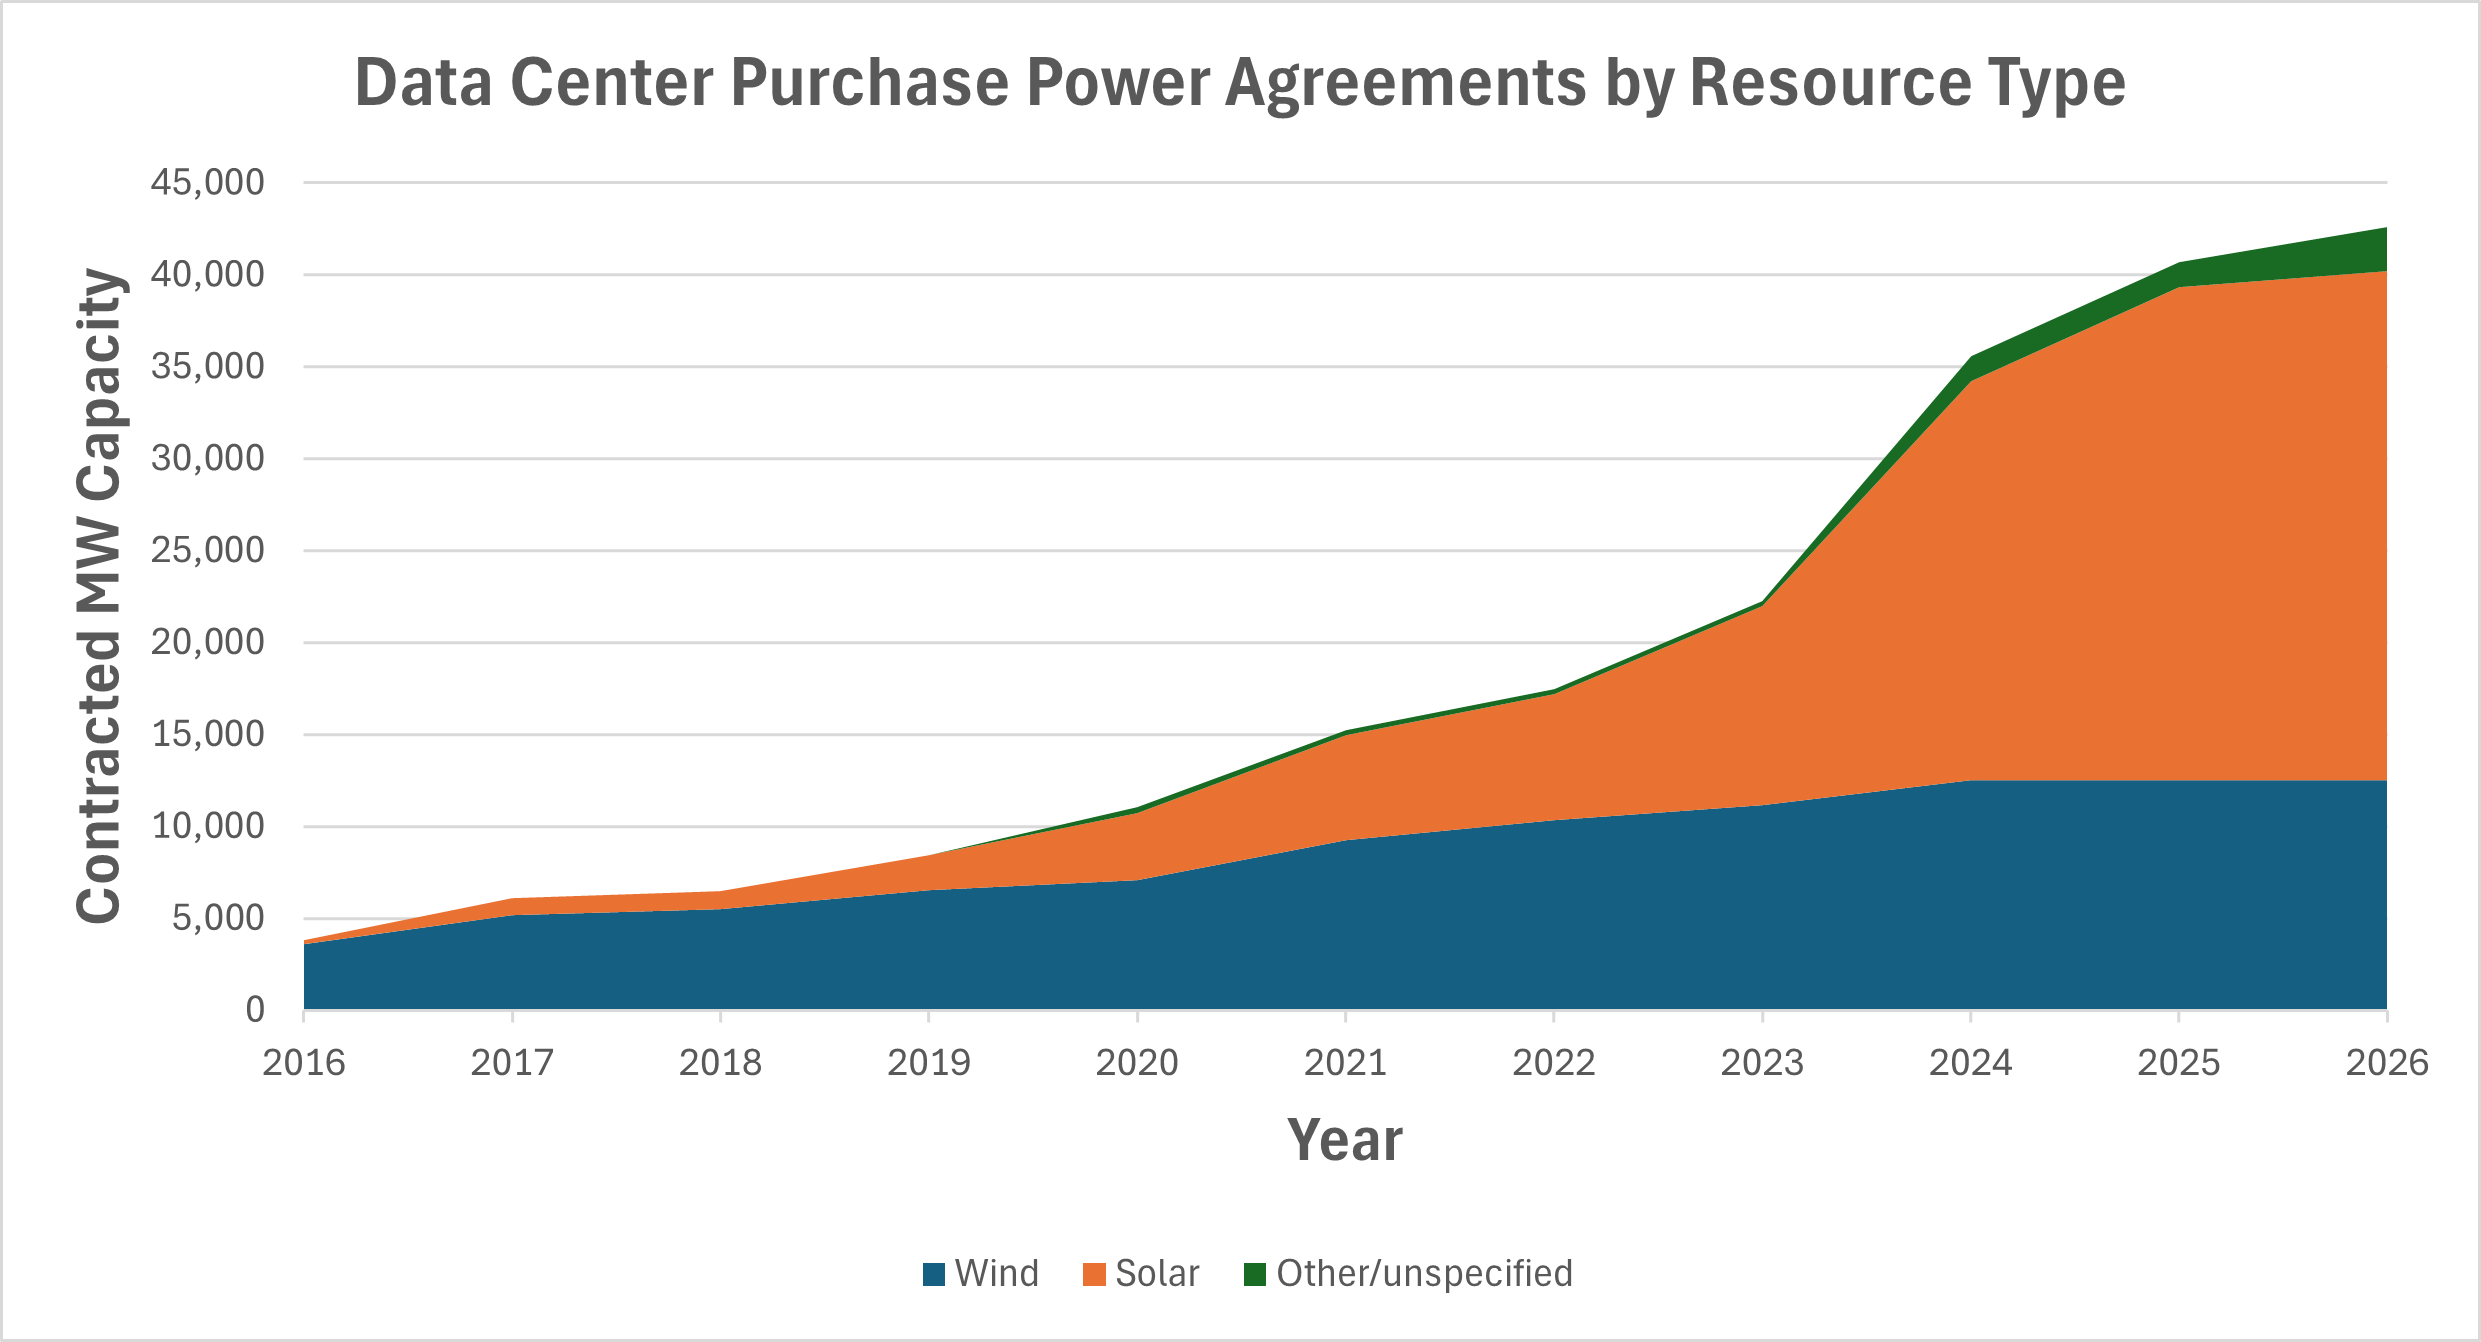
\includegraphics[width=0.75\linewidth]{Figures/PPA by Resource Type.png}
%     \caption{Data Center PPAs by Resource Type}
%     \label{fig:PPAbyResource}
% \end{figure}

% \begin{figure}
%     \centering
%     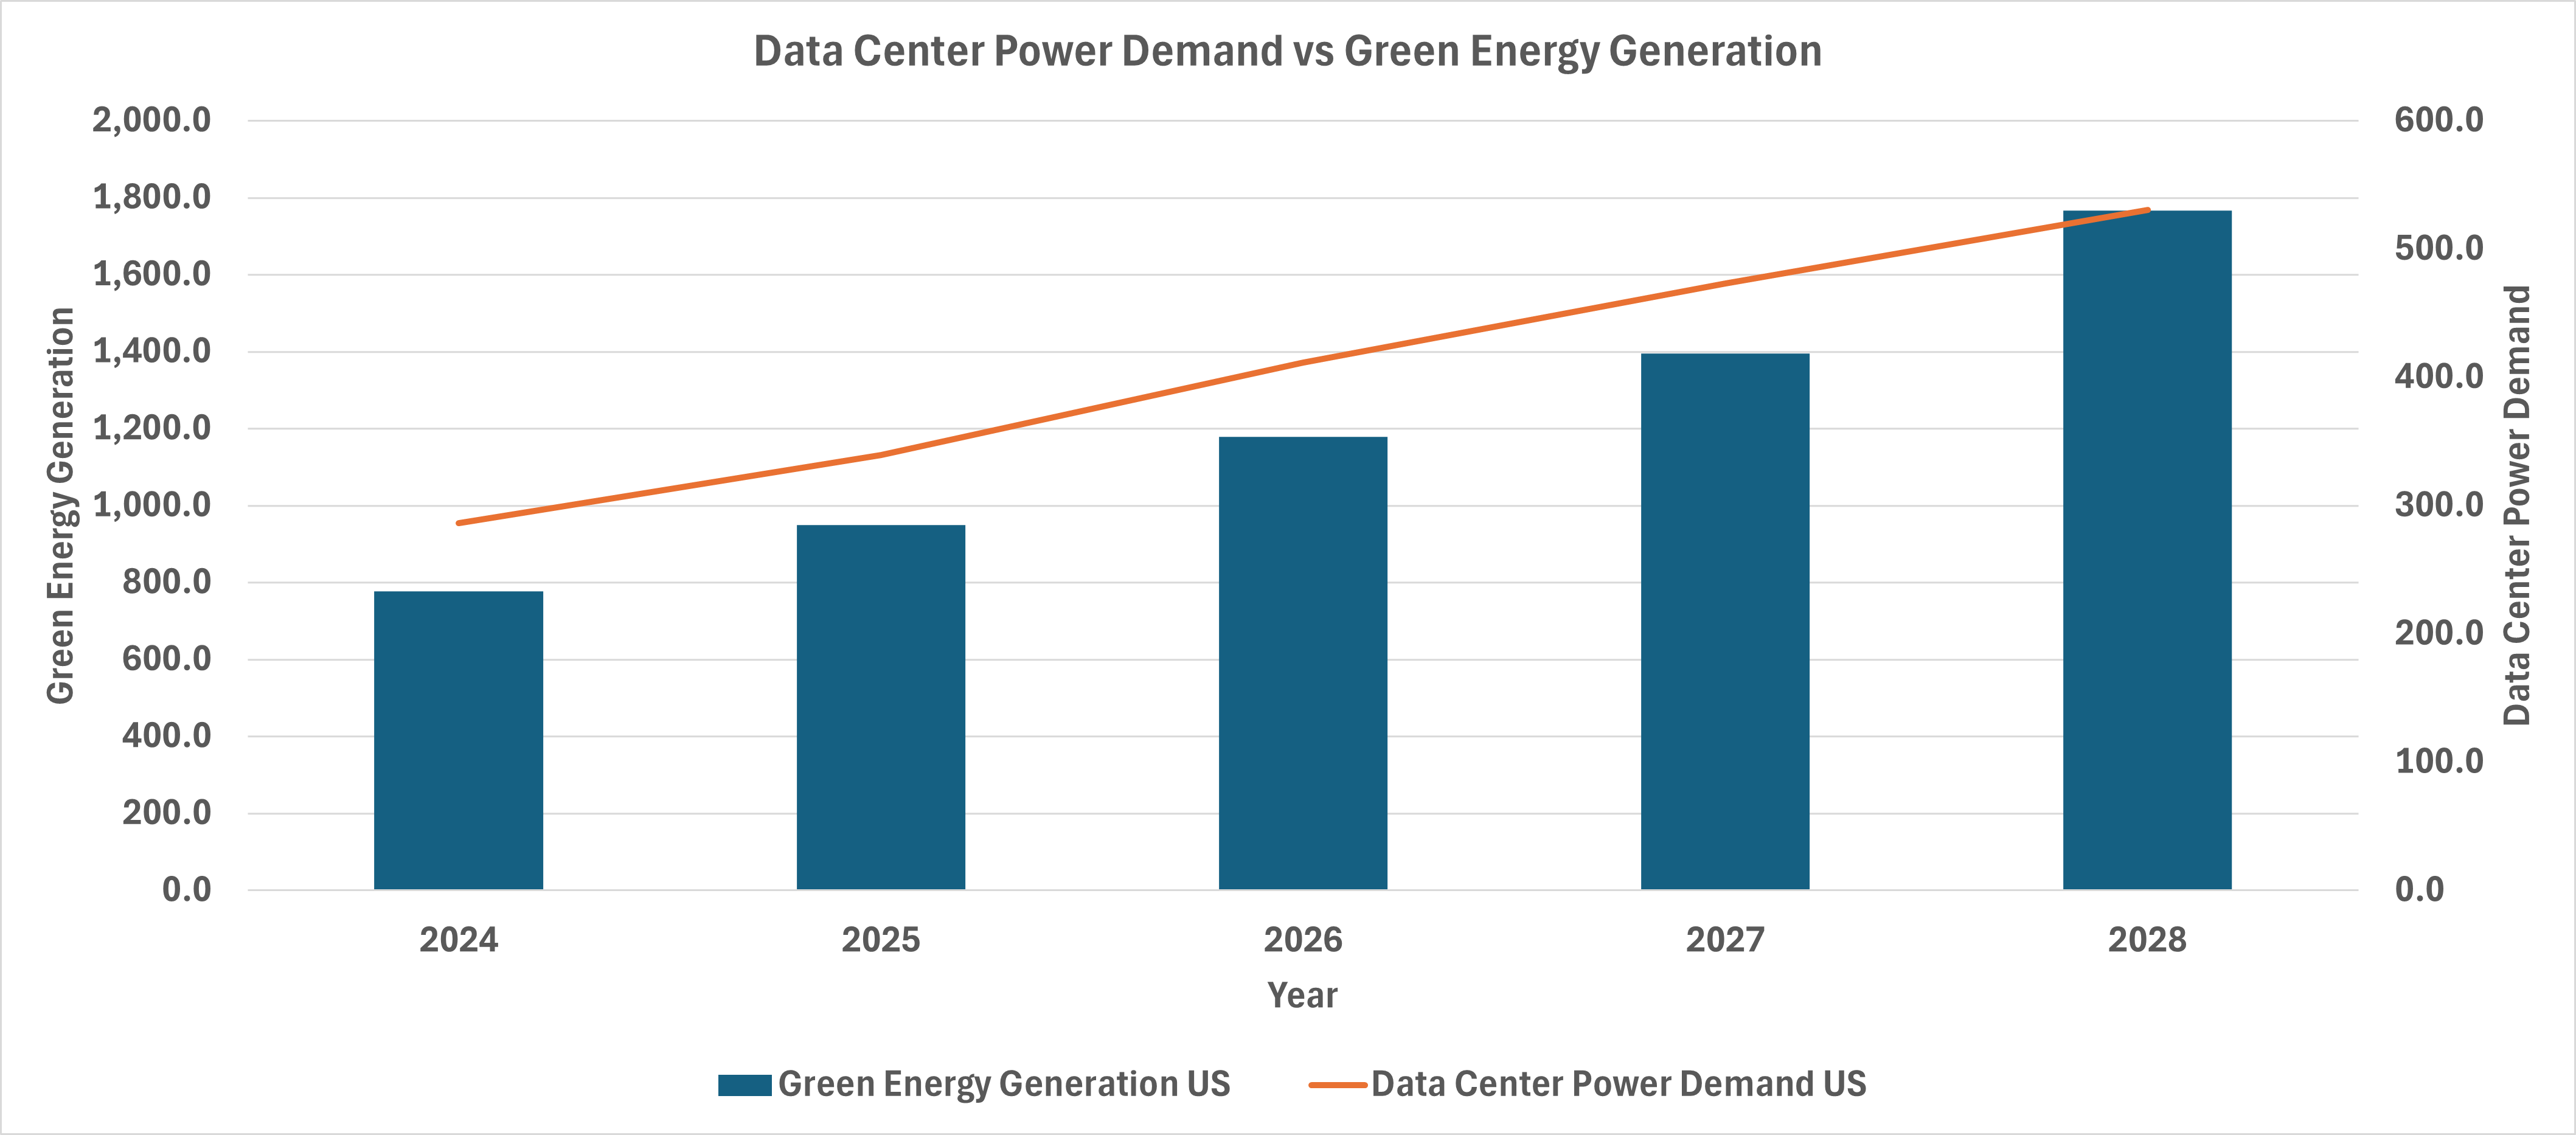
\includegraphics[width=0.5\linewidth]{Figures/Data Center Power Demand vs Green Generation.png}
%     \caption{Data Center Power Consumption vs Green Generation. Source: Aterio.io}
%     \label{fig:DCPowerConsumption}


\section{Results}\label{Sec::Results}
%We first present main results that quantify the power quality~\autoref{subsec:power-quality-results}, fossil fuel demand~\autoref{subsec:fossil-fuel-demand-results}, and price effects~\autoref{subsec:price-effects-results} of training and running AI models on data centers. Then, we present the statistical robustness checks on the validity of the approach, and  

We reports results using our stacked DiD estimator (\autoref{subsec:eventstudy}) which is designed to handle staggered AI model releases. For all power quality and fossil demand effects, we first construct cohort-specific datasets following \citet{callaway2021difference}, for each of the treatment events corresponding to major AI model releases through 2023 (\autoref{appendix:verified-models}).
Table \ref{tab:combined_results} provides the full set of results from our main regressions including analysis of the impacts of on-site colocated generation for our counterfactuals.

\begin{table*}[t]
\centering
\caption{Summary of Estimation Results Across Specifications}
\label{tab:combined_results}
\begin{tabular}{llcp{10cm}}
\toprule
Analysis & Outcome & Coefficient & Coefficient (Effect) Interpretation \\
\midrule
\multicolumn{4}{l}{\textit{Panel A: Utility-Level Power Quality (Two-Way FE)}} \\
\addlinespace[0.5em]
Strict DiD & CPQI & 0.3795*** & Corresponds to moving from typical U.S. power quality to the bottom quartile; increases annual outages for the average customer from 1 to $\sim$1.5–2. \\
Strict DiD & THD ($>$0.8) & 0.0625*** & Causes more outages and equipment failure. \\
\addlinespace[0.5em]
\midrule
\multicolumn{4}{l}{\textit{Panel B: Generator-Level Demand (Stacked DiD)}} \\
\addlinespace[0.5em]
%OLS & Pre-treatment avg & +1.28 & \multirow{4}{7.5cm}{Aggregate impact represents over 500 additional GWh near data centers over the inference period—equivalent to $\sim$47,000 U.S. household-years of consumption, with uneven load distribution across hours} \\
%OLS & Post-treatment avg & $-1.57$ & \\
IV 2SLS & Pre-treatment avg & +6.33*** & \multirow{4}{7.5cm}{$>500$ additional GWh; $\sim$47,000 household-years} \\
IV 2SLS & Post-treatment avg & +5.20*** & \\
\addlinespace[0.5em]
\midrule
\multicolumn{4}{l}{\textit{Panel C: PJM AI Price Analysis}} \\
\addlinespace[0.5em]
ComEd & Supply Elasticity & 31.64 & \multirow{2}{7.5cm}{Higher supply elasticity in ComEd zone corresponds to larger AI-induced price impacts; AEP's lower elasticity yields substantially smaller price effects} \\
ComEd & AI Price Impact & 25.39 & \\
AEP & Supply Elasticity & 8.13 & \\
AEP & AI Price Impact & 1.89 & \\
\addlinespace[0.5em]
\midrule
\multicolumn{4}{l}{\textit{Panel D: Power Quality by On-Site Generation Status}} \\
\addlinespace[0.5em]
With on-site & CPQI & $-0.122$*** & \multirow{3}{7.5cm}{On-site generation mitigates grid stress from AI load; utilities without on-site experience reliability deterioration while those with on-site see improvements} \\
Without on-site & CPQI & +0.228*** & \\
Difference & CPQI & $-0.350$*** & \\
\bottomrule
\end{tabular}
\begin{flushleft}
\footnotesize\textit{Notes:} *** $p < 0.001$, ** $p < 0.05$. Panel A: Utility and time fixed effects with cluster-robust standard errors; treatment defined as presence of AI-affiliated data center in utility service territory. Panel B: 35.6 million observations from 19 treatment events; standard errors clustered by unit-event; IV instruments: natural gas price $\times$ zone-average heat rate. OLS = Ordinary Least Squares; IV 2SLS= Instrumental Variables Two Stage Least Squares; CPQI = Consumer Power Quality Index; THD = Total Harmonic Distortion. 
\end{flushleft}
\end{table*}

\subsection{Power Quality Effects: Utility-Level Strict DiD}\label{subsec:power-quality-results}

We report the power quality effects of AI data centers in seventy one retail electric utility service territories estimated from power quality observations over 1136 utility-months. We use Consumer Power Quality Index (CPQI) and Total Harmonic Distortion (THD) as outcome variables in our stacked DiD models (~\autoref{eq:pq_eventstudy}). 

Panel A in Table~\ref{tab:combined_results} reports results from the utility-level strict DiD specification. We use strict here to distinguish that due to the sample size, we prefer the traditional DiD as our main specification rather than the stacked alternative.
% \nb{why are we suddently mentioning \textbf{strict} DiD here? Discuss what it means earlier somewhere or at the very least describe here}.
The estimated CPQI coefficient speaks to the reliability of the power supply to the consumers. The CPQI coefficient of 0.3795 indicates a power quality deterioration level that corresponds to moving from a typical U.S. power area toward the bottom quartile of power quality—roughly \textbf{the difference between $\sim$ 1 outage/year and $\sim$ 1.5–2 outages/year for the average customer}. Other reliability events such as brownouts and surges are predicted to increase by ~1-2 per year. Importantly, power surges are a known ignition source for electrical fires, contributing to the approximately 51,000 annual residential electrical fires in the U.S., with electrical arcing accounting for 74\% of ignition sources \cite{usfa2019electrical}. 
%Fewer fires is generally considered a desirable outcome amongst electricity professionals \cite{Laughner2024THD}.
%\nb{Add brownouts or other reliability events}
% \footnote{These are calculated based on Whisker Labs description of the CPQI Score with a description of derivation in the appendix.} This implies more frequent voltage anomalies that make motors and electronics run less efficiently and age faster.



The post-treatment coefficient of 0.0625 for THD indicates that utility territories containing AI data centers experienced a 0.0625 percentage point increase in readings above the 0.8 distortion threshold following AI model releases. 
%\nb{A 0.06\% increase reads negligible. Can we add something that makes the impact clearer, likely, and concrete. For example you could say: While a fraction of a percentage point might seem a negligible effect, in practice this level of increase can cause substantial problems. For example, this level of increase will halve the lifespan of ....} 
While a 0.0625 percentage point increase may appear small in isolation, it is still problematic as sustained exposure to power distortions compounds to over the multi-year lifespans of household appliances, accelerating degradation of refrigerators, air conditioners, and other motor-driven equipment \cite{NEMA_MG1,Laughner2024THD}.
%, the IEEE 519 standard exists precisely because even modest increases in harmonic distortion impose continuous thermal stress on motor windings.According to the Arrhenius equation underlying motor insulation ratings, every 10°C rise in operating temperature halves insulation life \cite{NEMA_MG1}. Since elevated THD causes motors to waste additional power as heat in their iron and copper windings \cite{Laughner2024THD}, sustained exposure compounds over the multi-year lifespans of household appliances, accelerating degradation of refrigerators, air conditioners, and other motor-driven equipment.

%(\nb{e.g. reducing the lifespan of a microwave by X}).

%indicates that the surrounding area can expect an additional reliability event per year. This level of deterioration in CPQI corresponds to moving from a typical U.S. area toward the bottom quartile of power quality—roughly \textbf{the difference between $\sim$ 1 outage/year and $\sim$ 1.5–2 outages/year for the average customer}\footnote{These are calculated based on Whisker Labs description of the CPQI Score with a description of derivation in the appendix.}—and implies more frequent voltage anomalies that make motors and electronics run less efficiently and age faster. \nb{Can we also add something about how much faster a specific appliance (say a microwave) could age under this level of power quality deterioration?}


% \begin{table}[h]
% \centering
% \caption{Utility-Level Power Quality Results: Two-Way Fixed Effects (Strict DiD) along with the quality of fit metric ($R^2$).  \nb{Get rid of N and SE}}
% \label{tab:thd_results}
% \begin{tabular}{lcccc}
% \toprule
% Outcome & Post Coefficient & SE & $R^2$ & N \\
% \midrule
% THD ($>$0.8 threshold) & 0.0625*** & $<$0.001 & 0.956 & 1,136 \\
% CPQI & 0.3795*** & $<$0.001 & 0.956 & 1,136 \\
% \bottomrule
% \end{tabular}
% \begin{flushleft}
% \footnotesize\textit{Notes:} *** p < 0.001. Utility and time fixed effects with cluster-robust standard errors. Treatment defined as presence of AI-affiliated data center in utility service territory.
% \end{flushleft}
% \end{table}

\subsection{Fossil Fuel Demand Effects: Stacked DiD}
\label{subsec:fossil-fuel-demand-results}
 Fossil fuel demand effects are estimated using demand data from a total of 35.6 million generator-hour observations\footnote{These data are from he Clean Air Markets Program (CAMPD) dataset and include hourly generation by all US utility-scale fossil generators \cite{EPA_CAPMD_PowerSector2022.}}, which includes 900,956 treated observations from generators located within 20 miles of AI-affiliated data centers and the other 34.7 million from other generators as control observations.


%All specifications include zone and month fixed effects with standard errors clustered by unit-event. \nb{Dana, not sure if the previous sentence is important. I dont grok it readily and feels like something that can be omitted.} DG: In theory, it is important. Some economists would care a lot and be very happy we include FEs, but I think it's not a huge deal to omit it. \nb{Ok. If this is better said than not, then say it somewhere relevant in the appendix. No issues if not.}
%Further details on the instrumental variables specification can be found in Appendix Subsection \ref{IVDetails}. 

Average fossil fuel demand effects are shown in the IV 2SLS rows in Panel B of Table~\ref{tab:combined_results}.\footnote{Recall that we use two stage instrumental variables (IV) regression here, where the second stage isolates the AI model caused demand-side effects from supply shocks (i.e., generator heat rate and alternate fuel source prices) modeled in the first stage. Details on the specifics of the instrumental variables specification can be found in Appendix Subsection \ref{IVDetails} and results from the first stage regression are presented in Appendix.}  Figure \ref{fig:event_study_main} shows the coefficients spread two months before (training) and after (inference) model release.

%over two months prior to the release (training) and two months after (inference). 

The training phase fossil fuel power demand corresponds to the $t=-2$ pre-treatment coefficient of $6.33$ MWh, which we find to also be statistically significant result. Note that this is the hourly demand at a single generator.  When the aggregate impact is calculated, they represent over 500 additional GWh added nearby to a data center over the inference period in some cases. \textbf{The additional power is roughly equivalent to that of 47,000 household-years in the United States}. For inference, the $t=+2$ coefficient shows a significant demand increase of 5.20 MWh, representing the demand shift at generators near data centers two months after AI model release, isolated from supply-side price variation through our instrumentation strategy. 



%The pre-treatment coefficient at $t=−2$ is highly significant, representing demand created by training. Note that co-efficients denote hourly demand shift for a single generator.

% \begin{table}[h]
% \centering
% \caption{Stacked DiD Coefficients: Generator-Level Demand}
% \label{tab:event_study}
% \begin{tabular}{lccccc}
% \toprule
% & \multicolumn{2}{c}{OLS} & & \multicolumn{2}{c}{IV 2SLS} \\
% \cmidrule{2-3} \cmidrule{5-6}
% Event Time & Coefficient & SE & & Coefficient & SE \\
% \midrule
% $t = -2$ & +1.28 & (1.29) & & +6.33*** & (1.63) \\
% $t = -1$ & \multicolumn{2}{c}{[reference]} & & \multicolumn{2}{c}{[reference]} \\
% $t = 0$ & $-4.39$ & (3.10) & & +0.69 & (2.79) \\
% $t = +1$ & $-1.64$ & (2.80) & & +0.74 & (2.45) \\
% $t = +2$ & +1.31 & (2.27) & & +5.20** & (2.54) \\
% \midrule
% Pre-treatment avg & \multicolumn{2}{c}{+1.28} & & \multicolumn{2}{c}{+6.33} \\
% Post-treatment avg & \multicolumn{2}{c}{$-1.57$} & & \multicolumn{2}{c}{+2.21} \\
% \bottomrule
% \end{tabular}
% \begin{flushleft}
% \footnotesize\textit{Notes:} *** p < 0.01, ** p < 0.05. N = 35.6 million observations from 19 treatment events. Standard errors clustered by unit-event. IV instruments: natural gas price $\times$ zone-average heat rate.
% \end{flushleft}
% \end{table}

% The OLS specification shows no significant effects in any period, consistent with the parallel trends validation. Figure \ref{fig:event_study_main} shows the stacked DiD coefficients for power demand in the 2SLS specification. The 2SLS specification reveals two notable patterns. First, the $t=-2$ coefficient is significant (6.33, p < 0.01) indicating a significant traning demand increase.. Second, the $t=+2$ coefficient shows a significant demand increase of 5.20 MWh (SE = 2.54, p < 0.05), representing the demand shift at generators near data centers two months after AI model release, isolated from supply-side price variation through our instrumentation strategy. While these effects may not seem large enough to be economically interesting, these effects are hourly and by generator. When the aggregate impact is calculated, they represent over 500 additional GWh added nearby to a data center over the inference period in some cases. \textbf{The additional power is roughly equivalent to that of 47,000 household-years in the United States}. This further strains grids as the power is not evenly distributed across hours. The pre-treatment coefficient at $t=-2$ is significant, representing demand created by training, but prior to treatment, the trends are identical with the control sample. Figure~\ref{fig:event_study_main} displays stacked DiD coefficients for the pre-treatment and post-treatment windows from the OLS specification. 
\begin{figure}[t]
    \centering
    % Note: Reference the actual output files from stacked_did_iv_results/
    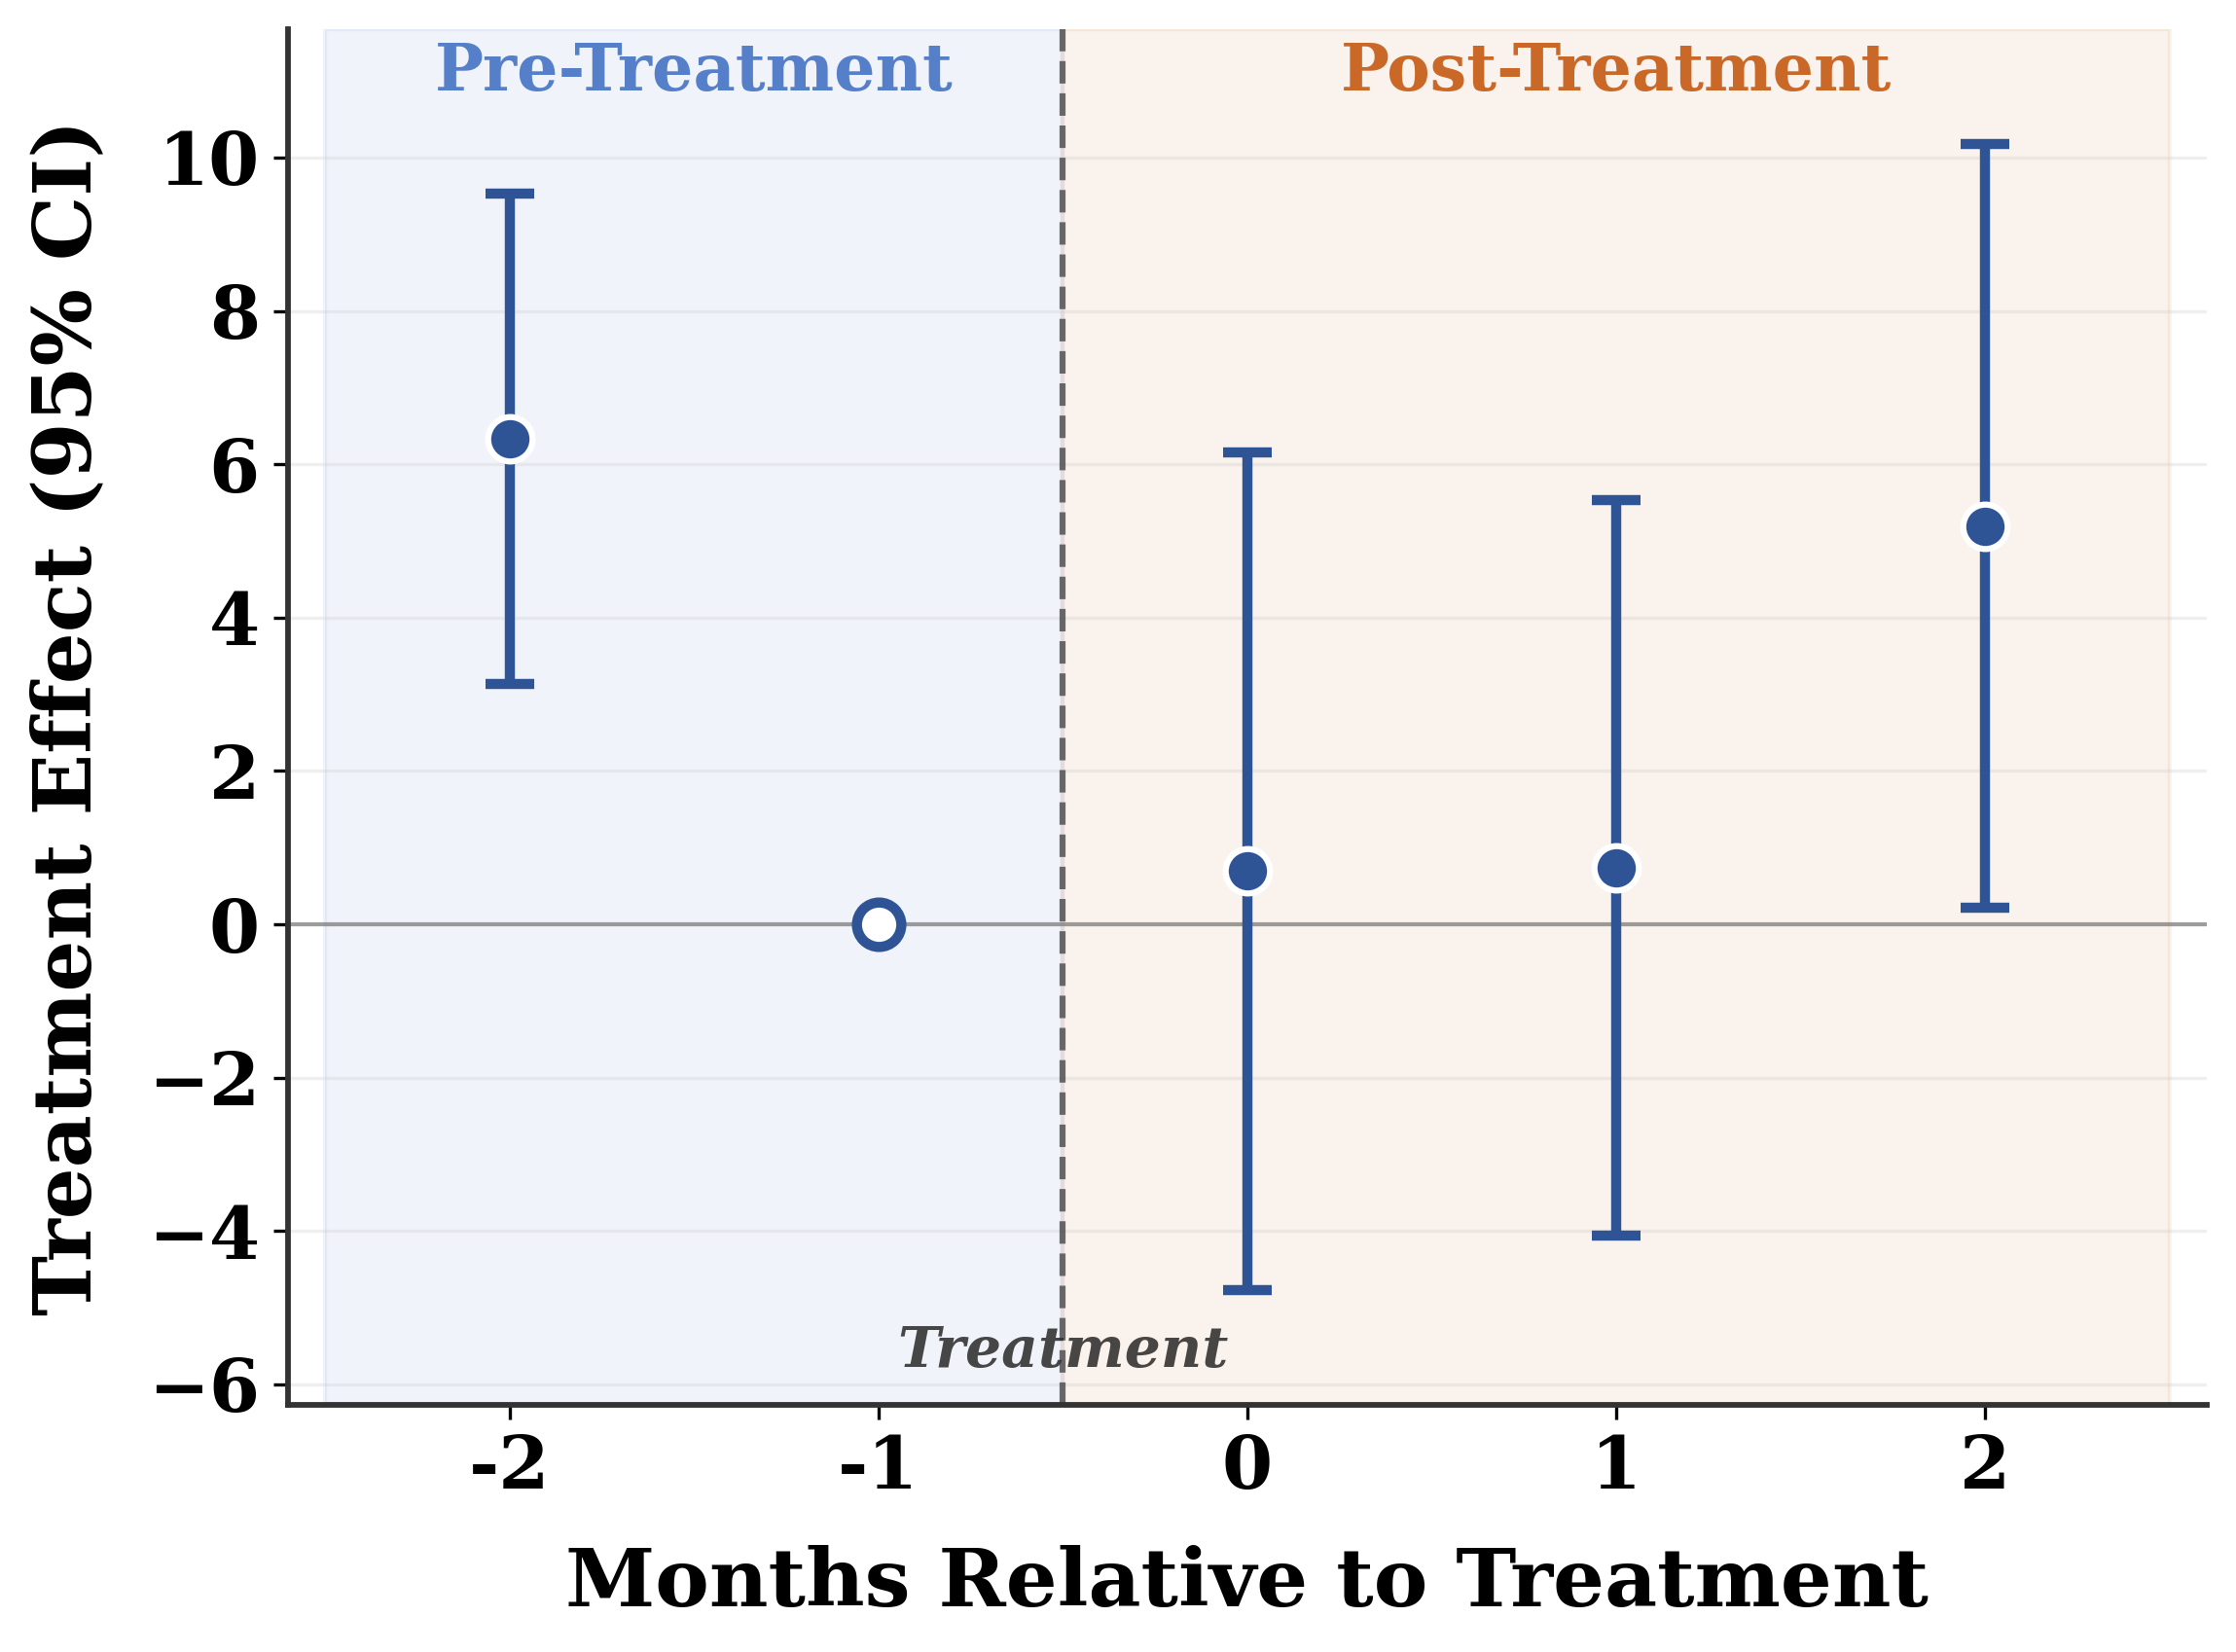
\includegraphics[width=0.7\linewidth]{Figures/event_study_figure.png}
    \caption{Stacked DiD coefficients for power demand (IV specification). Event Time 0 corresponds to AI model publication date. The pre-treatment coefficient at $t=-2$ demonstrates the training demand. Reference period is $t=-1$.}
    \Description{Plot showing stacked DiD coefficients for power demand, with event time 0 as AI model publication date.}
    \label{fig:event_study_main}
    \vspace{-2em}
\end{figure}



% \subsubsection{Parallel Trends Validation}

% We first assess the parallel trends assumption underlying our identification strategy.


\subsection{Price Impacts}
\label{subsec:price-effects-results}
% \nb{is there a reason why we use Impacts rather than Effects here?} DG: Mainly to vary language and also to avoid using the same word right after itself. I will change.
% We estimate wholesale electricity price impacts by combining our demand estimates with supply curve parameters, following the methodology outlined in Section \ref{PriceEffects}. This approach recognizes that our IV strategy identifies demand shifts but does not directly estimate equilibrium price effects\nb{expand this terminology as a footnote}. The price impact of AI-induced demand depends on the slope of the supply curve\nb{footnote explaining what this is}: inelastic supply\nb{expand this terminology} implies large price effects, while elastic supply implies small effects. Additional specifics on calculation methodology can be found in Appendix Subsection \ref{CalcMethodologyPrice}. 

We estimate wholesale electricity price effects by combining our demand estimates with supply curve parameters. This approach, described in Section \ref{PriceEffects}, recognizes that our IV strategy identifies demand shifts but does not directly estimate equilibrium price effects.\footnote{Our instrumental variables approach isolates exogenous variation in electricity demand driven by AI model releases. However, observed market prices reflect the intersection of supply and demand in equilibrium. To translate our demand estimates into price effects, we must incorporate information about supply-side responses, which requires additional assumptions about the shape of the supply curve.} The price impact of AI-induced demand depends on the slope of the supply curve\footnote{Recall, the supply curve describes the relationship between price and quantity supplied. Its slope reflects how much generators must be compensated to produce additional electricity—steeper slopes indicate that marginal generation costs rise quickly as output expands, typically because higher-cost units must be dispatched.}: inelastic supply, where quantity supplied responds weakly to price changes, implies large price effects, while elastic supply implies small effects. We use supply chain elasticities for PJM obtained from our supply-side instrumental variables regression (see Figure \ref{PJMPRiceElasticity} in Appendix \ref{PriceElasticityAppendix} for a map). 
%Additional specifics on calculation methodology can be found in Appendix Subsection \ref{CalcMethodologyPrice}.



Figure \ref{PJMPrice} showing price increase estimates by zone. On average AI training leads to \textbf{substantial increases in wholesale prices in PJM with the highest increase surpassing 25\% in the American Electric Power (AEP) Zone}.
%Additional caveats are provided in Appendix Subsection \ref{appendix:Caveats}

\begin{figure}[H]
    \centering    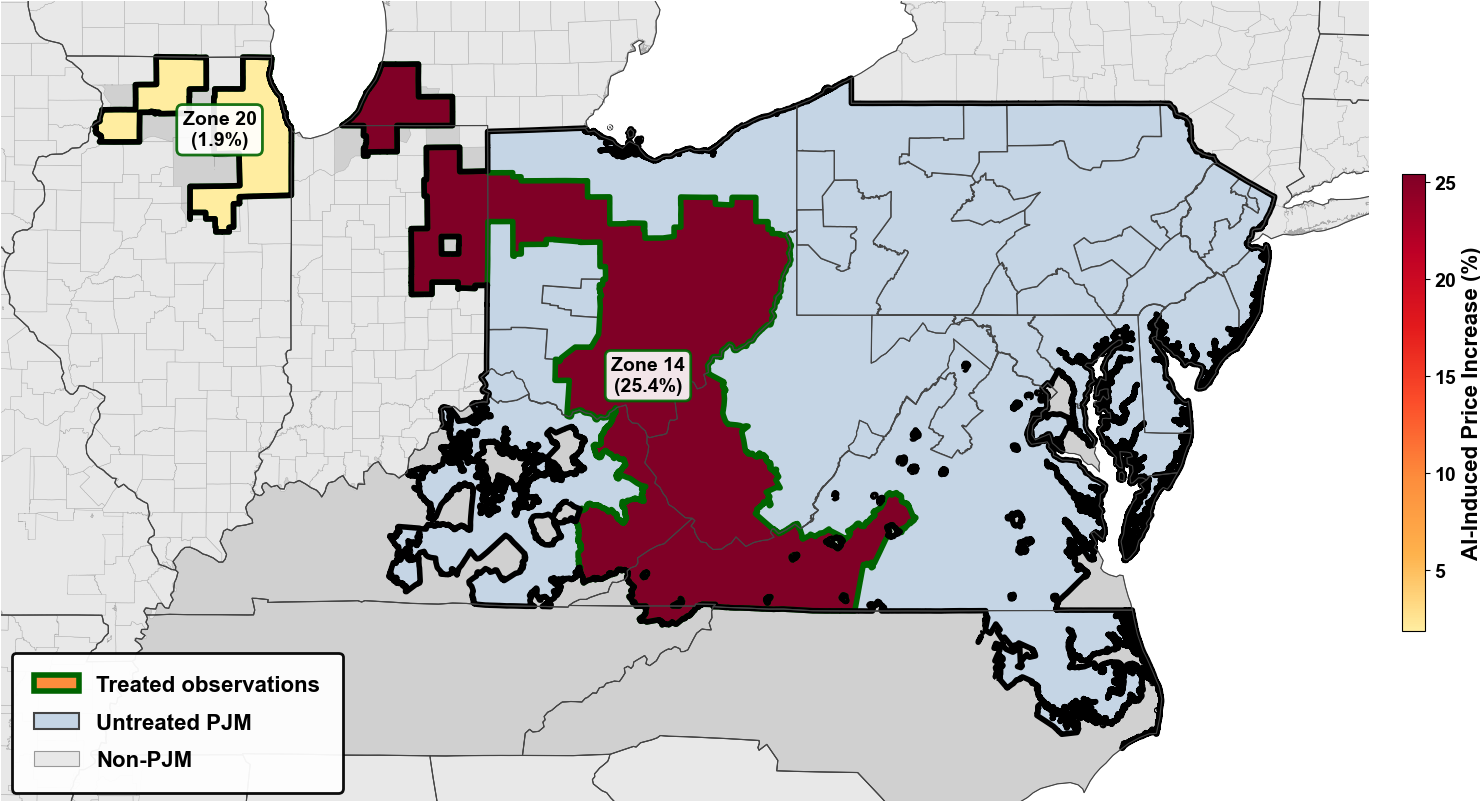
\includegraphics[width=0.5\linewidth]{Figures/PJMMap3.png}
    \caption{The map shows estimated AI-related wholesale prices increases in the PJM Interconnection in treated zones.}
    \label{PJMPrice}
    \vspace{-2em}
\end{figure}

%\nb{1) Expand caption to explain. 2) New figure showing the borders of where AI data centers are located..}

We also estimate the expected price rise for retail customers, using estimates from the literature as documented in Appendix Subsection \ref{WholesaleRetailPassthrough}. While we are not able to provide definite evidence of the impacts on retail price pass through, it should be noted that retail electricity prices have increased overall at a rate surpassing inflation since 2020 \cite{Nicoletti_Malik_Tartar_2024,horsley2025electricbill,spp2024stateofthemarket}. Also, while increased investment in electric generation through power purchase agreements by tech firms may in the long run lead to falling retail prices, it appears that at present data center power usage is increasing wholesale prices by raising total demand, which requires dispatching higher-cost generators and thus increases the market clearing price—a price paid by all retail consumers.

 Using the most relevant examples for PJM of retail elasticity of between .53 and .56 \cite{defeuilley2023pennsylvania}, \textbf{the expected consumer price rise in AEP, a sub-zone in PJM, would be $\sim 13\%$}. However, using recent long-run econometric estimates of full passthrough from \cite{mackay2024wholesale}, the long-run expected rise for consumers may be closer to the full 25\%.
% \section{Validating Assumptions and Robustness Checks}\label{Robustness}
\section{Validity and Robustness}\label{Robustness}
%Did the above to save space
% \nb{refer to earlier mention of issues}
%To address issues highlighted in Subsection \ref{DCASSUmptions}, we conduct several additional analyses to probe the robustness of our findings and explore effect heterogeneity i.e, the variance across different sub-groups in the data. 
We present two sets of analyses to address issues highlighted in Subsection \ref{DCASSUmptions}: formal testing to provide evidence for the parallel trends assumption, and placebo tests address potential issues related to external confounds or lack of specific knowledge about training. Additional tests are found in Appendix~\ref{App:AdditionalRobustnessChecks}.
%\nb{Dana, I lost the appendix number, please check:} 

\noindent\textbf{1) Formal Testing for Parallel Trends: } For power demand specifically, the formal joint test of pre-treatment coefficients using a Wald test of joint significance yields a chi-squared statistic of 0.99 (df = 1) with p-value = 0.3196. \textbf{We cannot reject the null hypothesis of parallel pre-trends at conventional significance levels.} This provides support for our assumption that treated and control generators followed similar demand trajectories prior to AI model releases i.e., our identification assumption is valid. Some of our samples demonstrate significant evidence against the the parallel trends test prior to propensity score matching (PSM) that we use for sample selection. However, across all matched samples for both power quality and power demand after PSM, we find \textit{no evidence of violations of the parallel trends assumption.}
%\nb{missingsomething here}.
This implies that the technique correctly handles the issue where it exists. 
 
 % Additionally, we estimate the baseline specification via OLS \nb{baseline specification via OLS doesn't grok. explain or drop baseline specification and instead say the first stage of the two stage IV regression or some such thing} to validate parallel trends prior to implementing our instrumental variables strategy. The OLS specification shows no significant effects in any period outside the training window, consistent with parallel trends holding in the pre-treatment period. Importantly, prior to treatment (excluding $t=-2$, which captures training demand), the trends are identical between treatment and control samples. Figure~\ref{fig:event_study_main} displays stacked DiD coefficients for both pre-treatment and post-treatment windows, with the reference period at $t=-1$. \nb{is the previous sentence necessary? we have discussed this figure already?}

\noindent\textbf{2) Placebo Tests}
We conduct two placebo exercises to demonstrate that the treatments are meaningful and not the result of random chance, we implement random date and random location placebo tests. Both yield a p-value of 1.00 for the coefficient in our fossil fuel demand, CPQI, and THD analyses, confirming that our results do not arise from spuriously chosen locations or dates.

%\nb{we dont use identification strategy earlier anymore; explain}.%First, to distinguish AI-specific effects from general data center growth, we estimate treatment effects using our 12,283 non-AI data centers as a placebo treatment group. If estimated effects simply reflect data center proximity rather than AI workloads specifically, we would expect similar magnitudes in this specification. The non-AI CPQI coefficient (0.228, p < 0.001) matches the AI data center coefficient for facilities without on-site generation, suggesting that general data center load---not AI workloads specifically---drives some of the observed power quality effects. 
%\nb{This previous statement seems to undercut the main point. We need to be careful that this isnt misunderstood. Actually I dont know if I understand what this says.}
% However, the demand-side 2SLS estimates from the stacked DiD, which leverage AI model release timing, remain distinct from this general data center effect.



% \subsubsection{Non-AI Data Center Placebo}

% To distinguish AI-specific effects from general data center growth, we estimate treatment effects using our 12,283 non-AI data centers as a placebo treatment group. If estimated effects simply reflect data center proximity rather than AI workloads specifically, we would expect similar magnitudes in this specification.

% The non-AI CPQI coefficient (0.228, p < 0.001) matches the AI data center coefficient for facilities without BTM generation, suggesting that general data center load---not AI workloads specifically---drives some of the observed power quality effects. However, the demand-side 2SLS estimates from the stacked event-study, which leverage AI model release timing, remain distinct from this general data center effect.

% \subsubsection{Random Dates and Random Locations Placebos}

% Both random dates and random locations yield a p-value of 1.00 for the coefficient in our fossil fuel demand, CPQI, and THD analyses. This suggests that our results are not the result of randmly chosen locations or dates.

\section{Counterfactual Analyses}
\label{sec:counterfactuals}

We present three main counterfactual exercises to inform stakeholders and policymakers about how alternative evolutionary paths for AI compute might affect grid outcomes. These combine our econometric estimates with data on model characteristics and infrastructure configurations to explore three dimensions: model scaling, geographic redistribution, and workload composition.\\

\noindent\textbf{1) Model Scaling.} We combine data on model size (parameter counts) with our econometric estimates from our least conservative specification to extrapolate grid impacts at different scales.

\noindent\textbf{(a) Power Quality.} Fitting a trend line to power quality impacts for Llama-3.1 (405B), PaLM (540B), and Llama 4 Behemoth (2T), we find that scaling from a 2 trillion parameter model to a 4 trillion parameter model would increase power quality impact from \textbf{0.321 to 0.434}---a deterioration of roughly 0.113 units, or just over 35\% relative to the 2 trillion baseline. The relationship is exponential over log parameter counts, implying that larger models require proportionally greater parameter reductions to achieve the same percentage improvement in power quality. \textbf{(b) Power Demand.} Using an analogous extrapolation, we find that \textbf{each 1\% parameter increase leads to approximately 0.15\% higher power demand} within three months of model release. Scaling from 540 billion to one trillion parameters would \textbf{increase total power demand by 10.5\%}. For DALL-E, halving parameters would \textbf{reduce inference demand by approximately 300 GWh}---equivalent to the annual consumption of 27,000--30,000 homes.\\

\noindent\textbf{2) Training Compute.} Training compute requirements also have measurable effects: a 1\% increase in training FLOPs is associated with a \textbf{0.1\% increase in power demand}. For GPT-3.5, halving training compute would reduce energy use by enough to power 8,000--10,000 U.S.\ homes for a year.\\

\noindent\textbf{3) Colocated On-site Generation.} Data centers increasingly deploy colocated on-site generation to reduce grid dependence. Our inventory identifies 87 facilities with on-site capability and 12,401 without. We test whether on-site capacity moderates estimated effects by interacting treatment with on-site status in the utility-level strict DiD specification. Results indicate that on-site generation substantially mitigates measured grid impacts. The sign reversal for CPQI is notable: data centers \textit{with} on-site generation are associated with improved power quality (negative coefficient), while those \textit{without} are associated with deterioration (positive coefficient). This heterogeneity suggests that \textbf{on-site generation absorbs demand spikes that would otherwise propagate to the grid}, and that aggregate grid impacts may understate total AI energy consumption.

Figure~\ref{fig:CounterfactualCombined} extends this to policy-relevant scenarios. Remarkably, universal adoption of on-site power would shift impact of data centers from a net detriment to power quality to a net improvement.\\
%However, all large AI data centers in our most conservative sample had on-site generation, which may exaggerate our estimates of colocated on-site generation's moderating effects.\nb{This statement again is a bit hard to parse. Does it undercut the impact statement above or support it?}

% \begin{figure}[h]
%     \centering
%     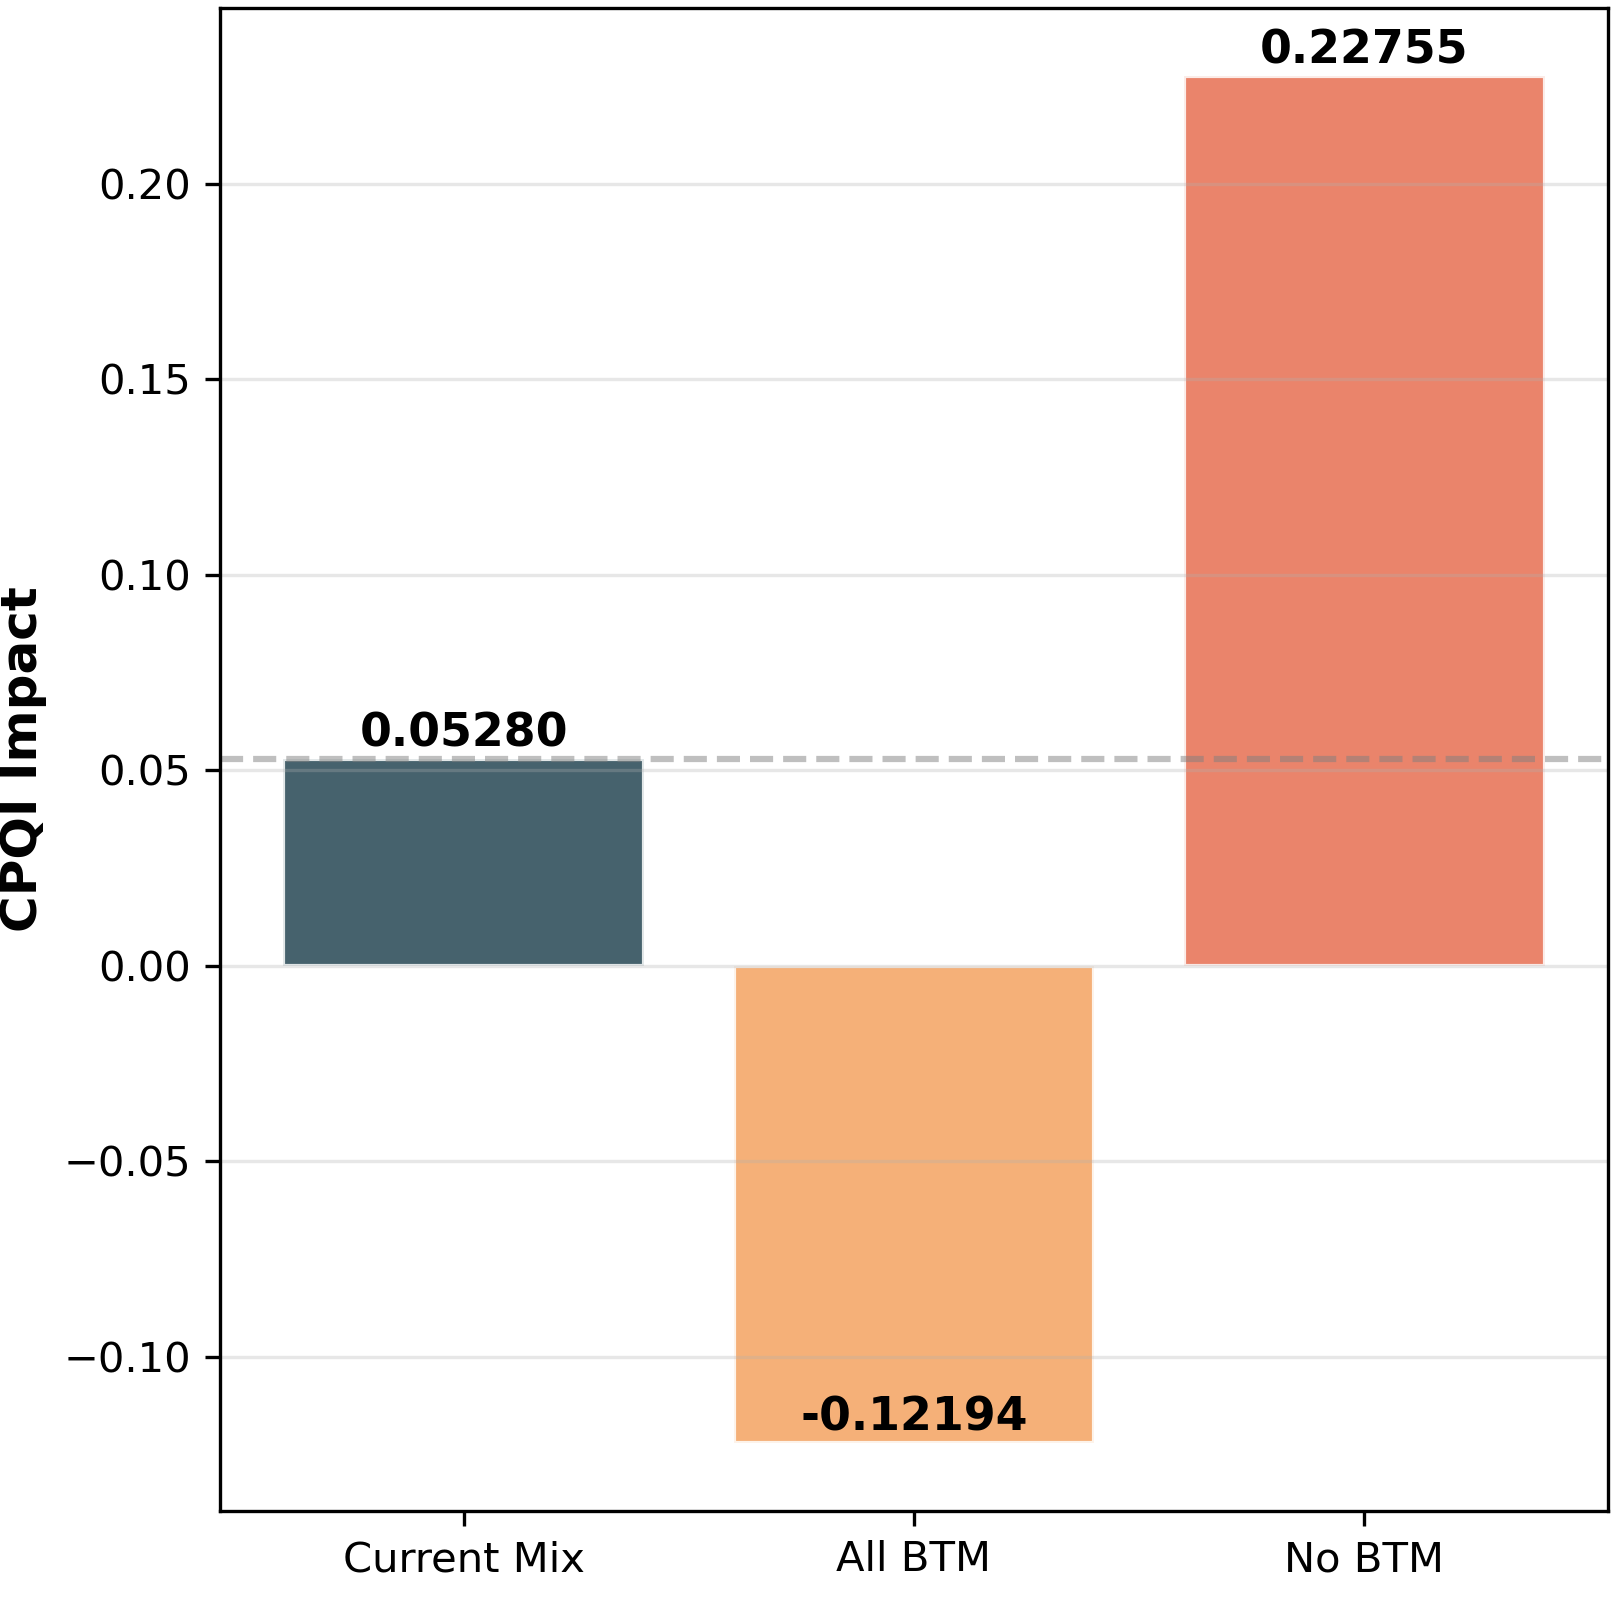
\includegraphics[width=0.35\linewidth]{Figures/btm_scenarios_analysis.png}
%     \caption{Impact of on-site power adoption on AI energy impacts.\nb{Dana it might be useful to collate plots in 5,6,and7 into a single figure laid side by side going across the two columns. this will save white space but also help make the figures bigger.}}
%     \label{fig:btm_scenarios}
% \end{figure}

\noindent\textbf{4) Geographic Redistribution}

%We analyze grid impacts under alternative spatial distributions of AI compute.

\noindent\textbf{(a) Distributed Inference (Edge Computing).} In our sample where we know AI data centers but not specific training and inference sites, we simulate a shift from cloud-based to edge-based inference, redistributing inference demand from concentrated hyperscaler facilities to smaller data centers located closer to population centers. Under this scenario, total demand added in a particular zone falls from a baseline of 162 MWh per hour over the entire treatment period to 4 MWh per hour. Figure~\ref{fig:CounterfactualCombined} illustrates this effect of shifting the composition of inference.

% \begin{figure}[h]
%     \centering
%     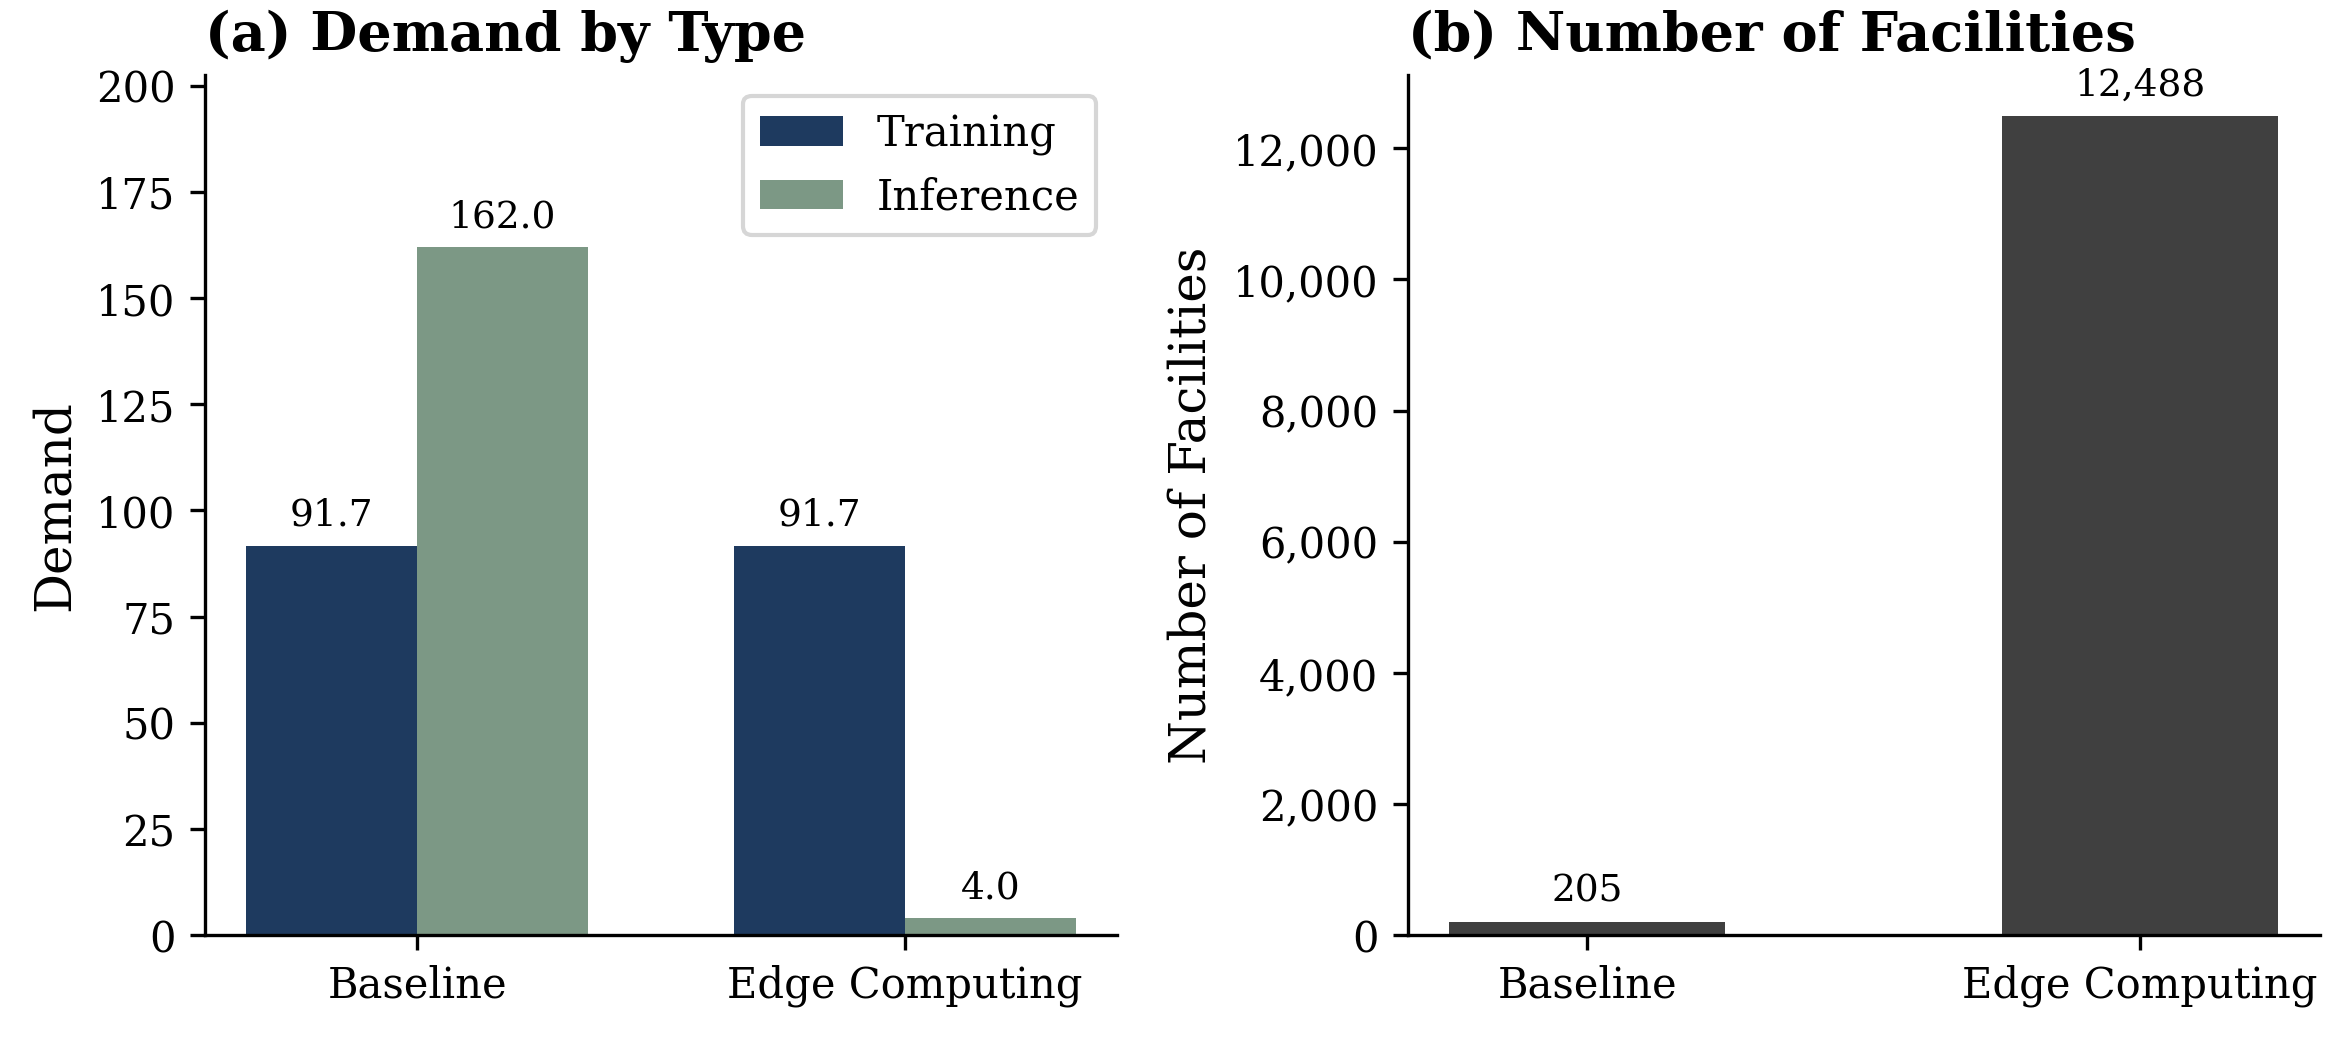
\includegraphics[width=0.5\linewidth]{Figures/CentralizedComputing.png}
%     \caption{Impact of distributing AI inference to edge data centers.}
%     \label{fig:edge_computing}
% \end{figure}

\noindent\textbf{(b) Concentration in Low-Population, High-Supply Regions.} Alternatively, we consider relocating both training and inference to regions with abundant electricity supply and lower baseline load, such as areas in the central United States with substantial renewable or fossil capacity. We simulate this by shifting demand from the baseline case where training and inference are assumed distributed to a case where the only data center for training and inference is the largest data center owned by a hyperscaler. This leads to an extreme concentration of added demand with nearly 100 GWh added near data centers in training locations. Figure~\ref{fig:CounterfactualCombined} shows this scenario.

This analysis has the important caveat that shifting to one data center for all training activity is extreme, with many possible configurations between full decentralization and full centralization. Centralization may also yield other benefits, such as concentration near renewable generation and reduced energy consumption from lower communication costs.

% \begin{figure}[h]
%     \centering
%     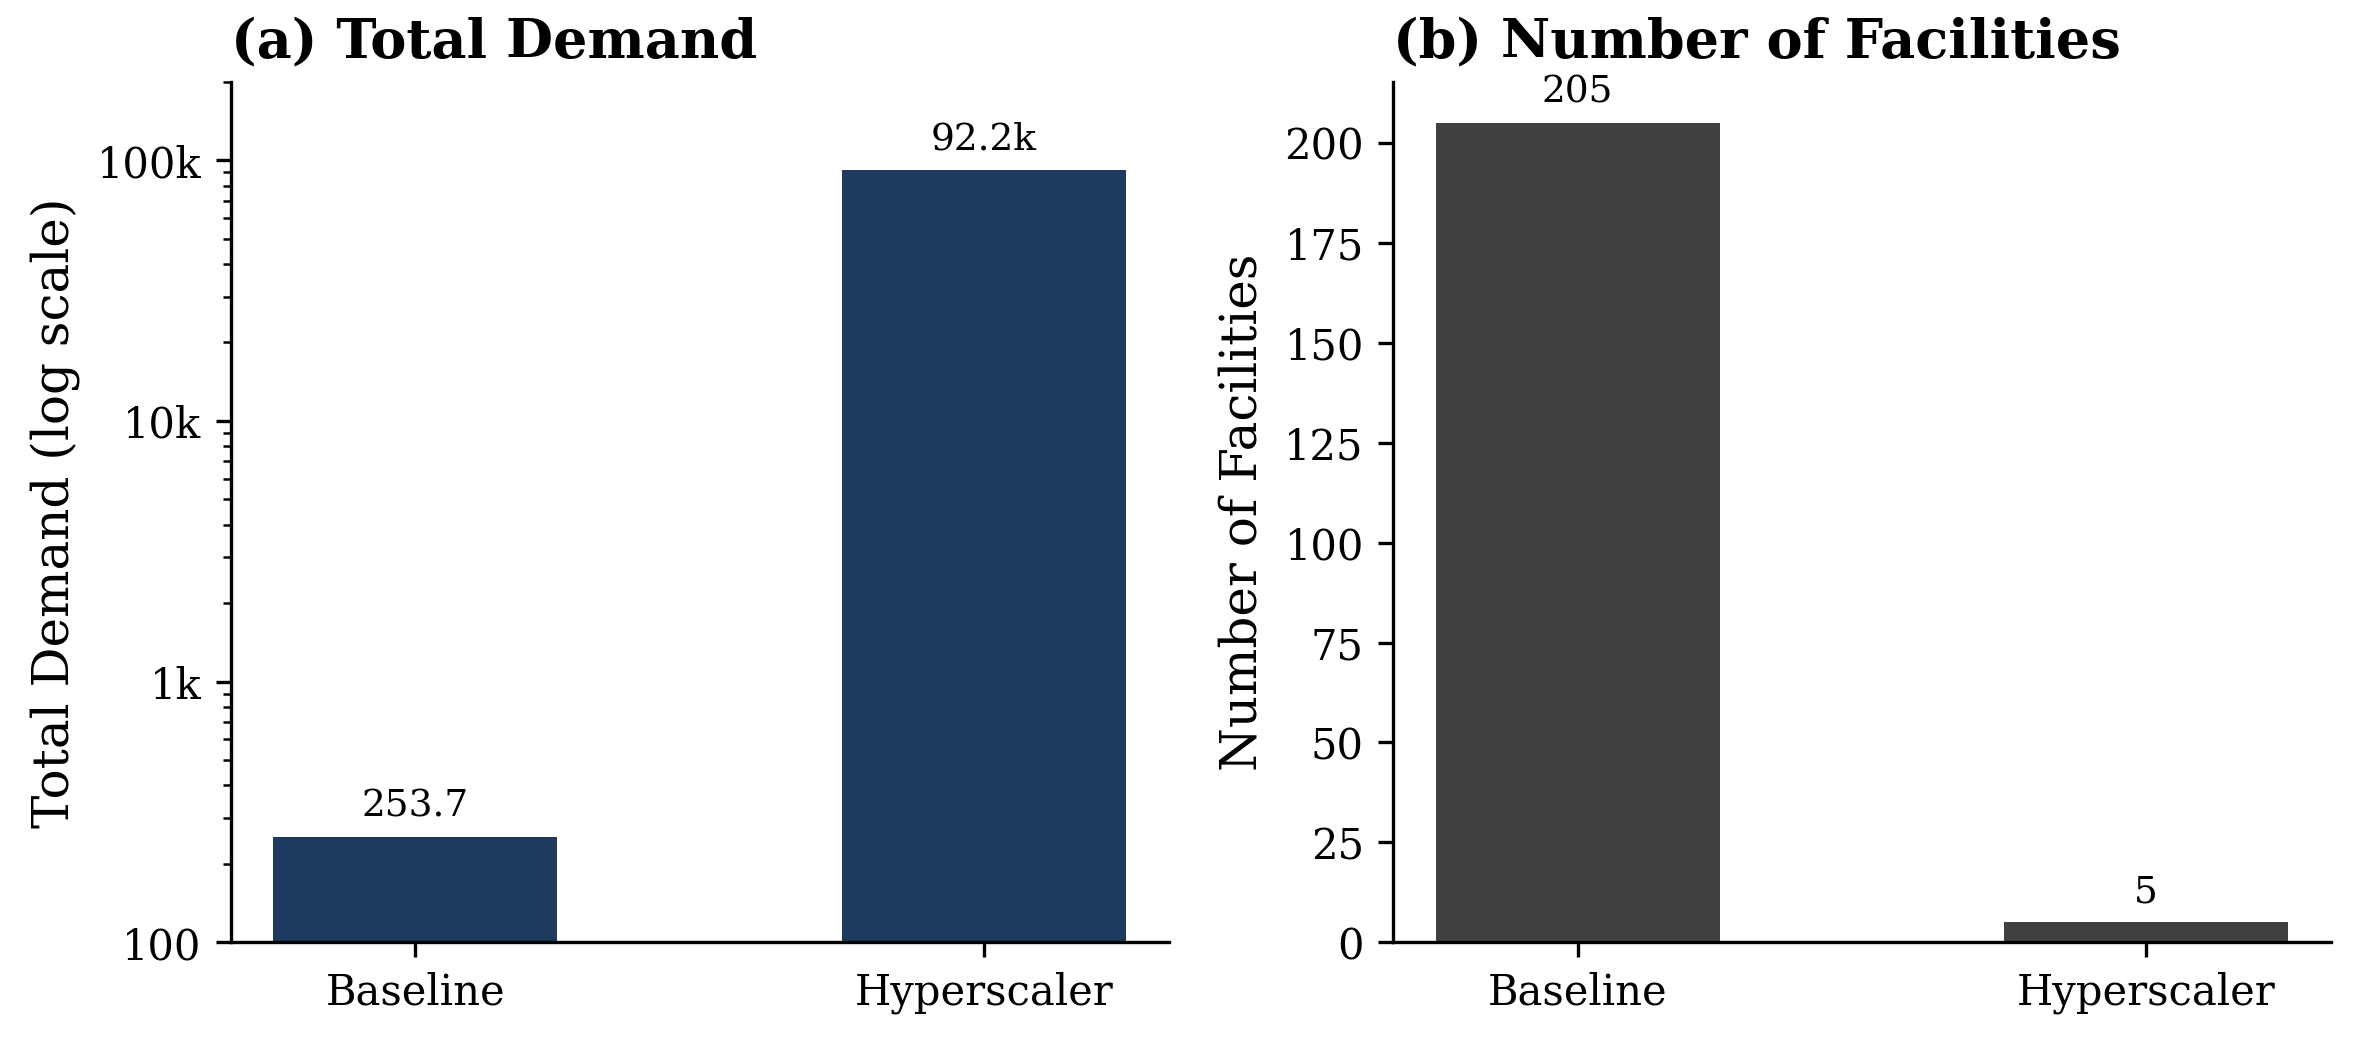
\includegraphics[width=0.5\linewidth]{Figures/Central.png}
%     \caption{Impacts of centralized computing to largest data center by hyperscaler.}
%     \label{fig:centralized_computing}
% \end{figure}

\begin{figure}
    \centering
    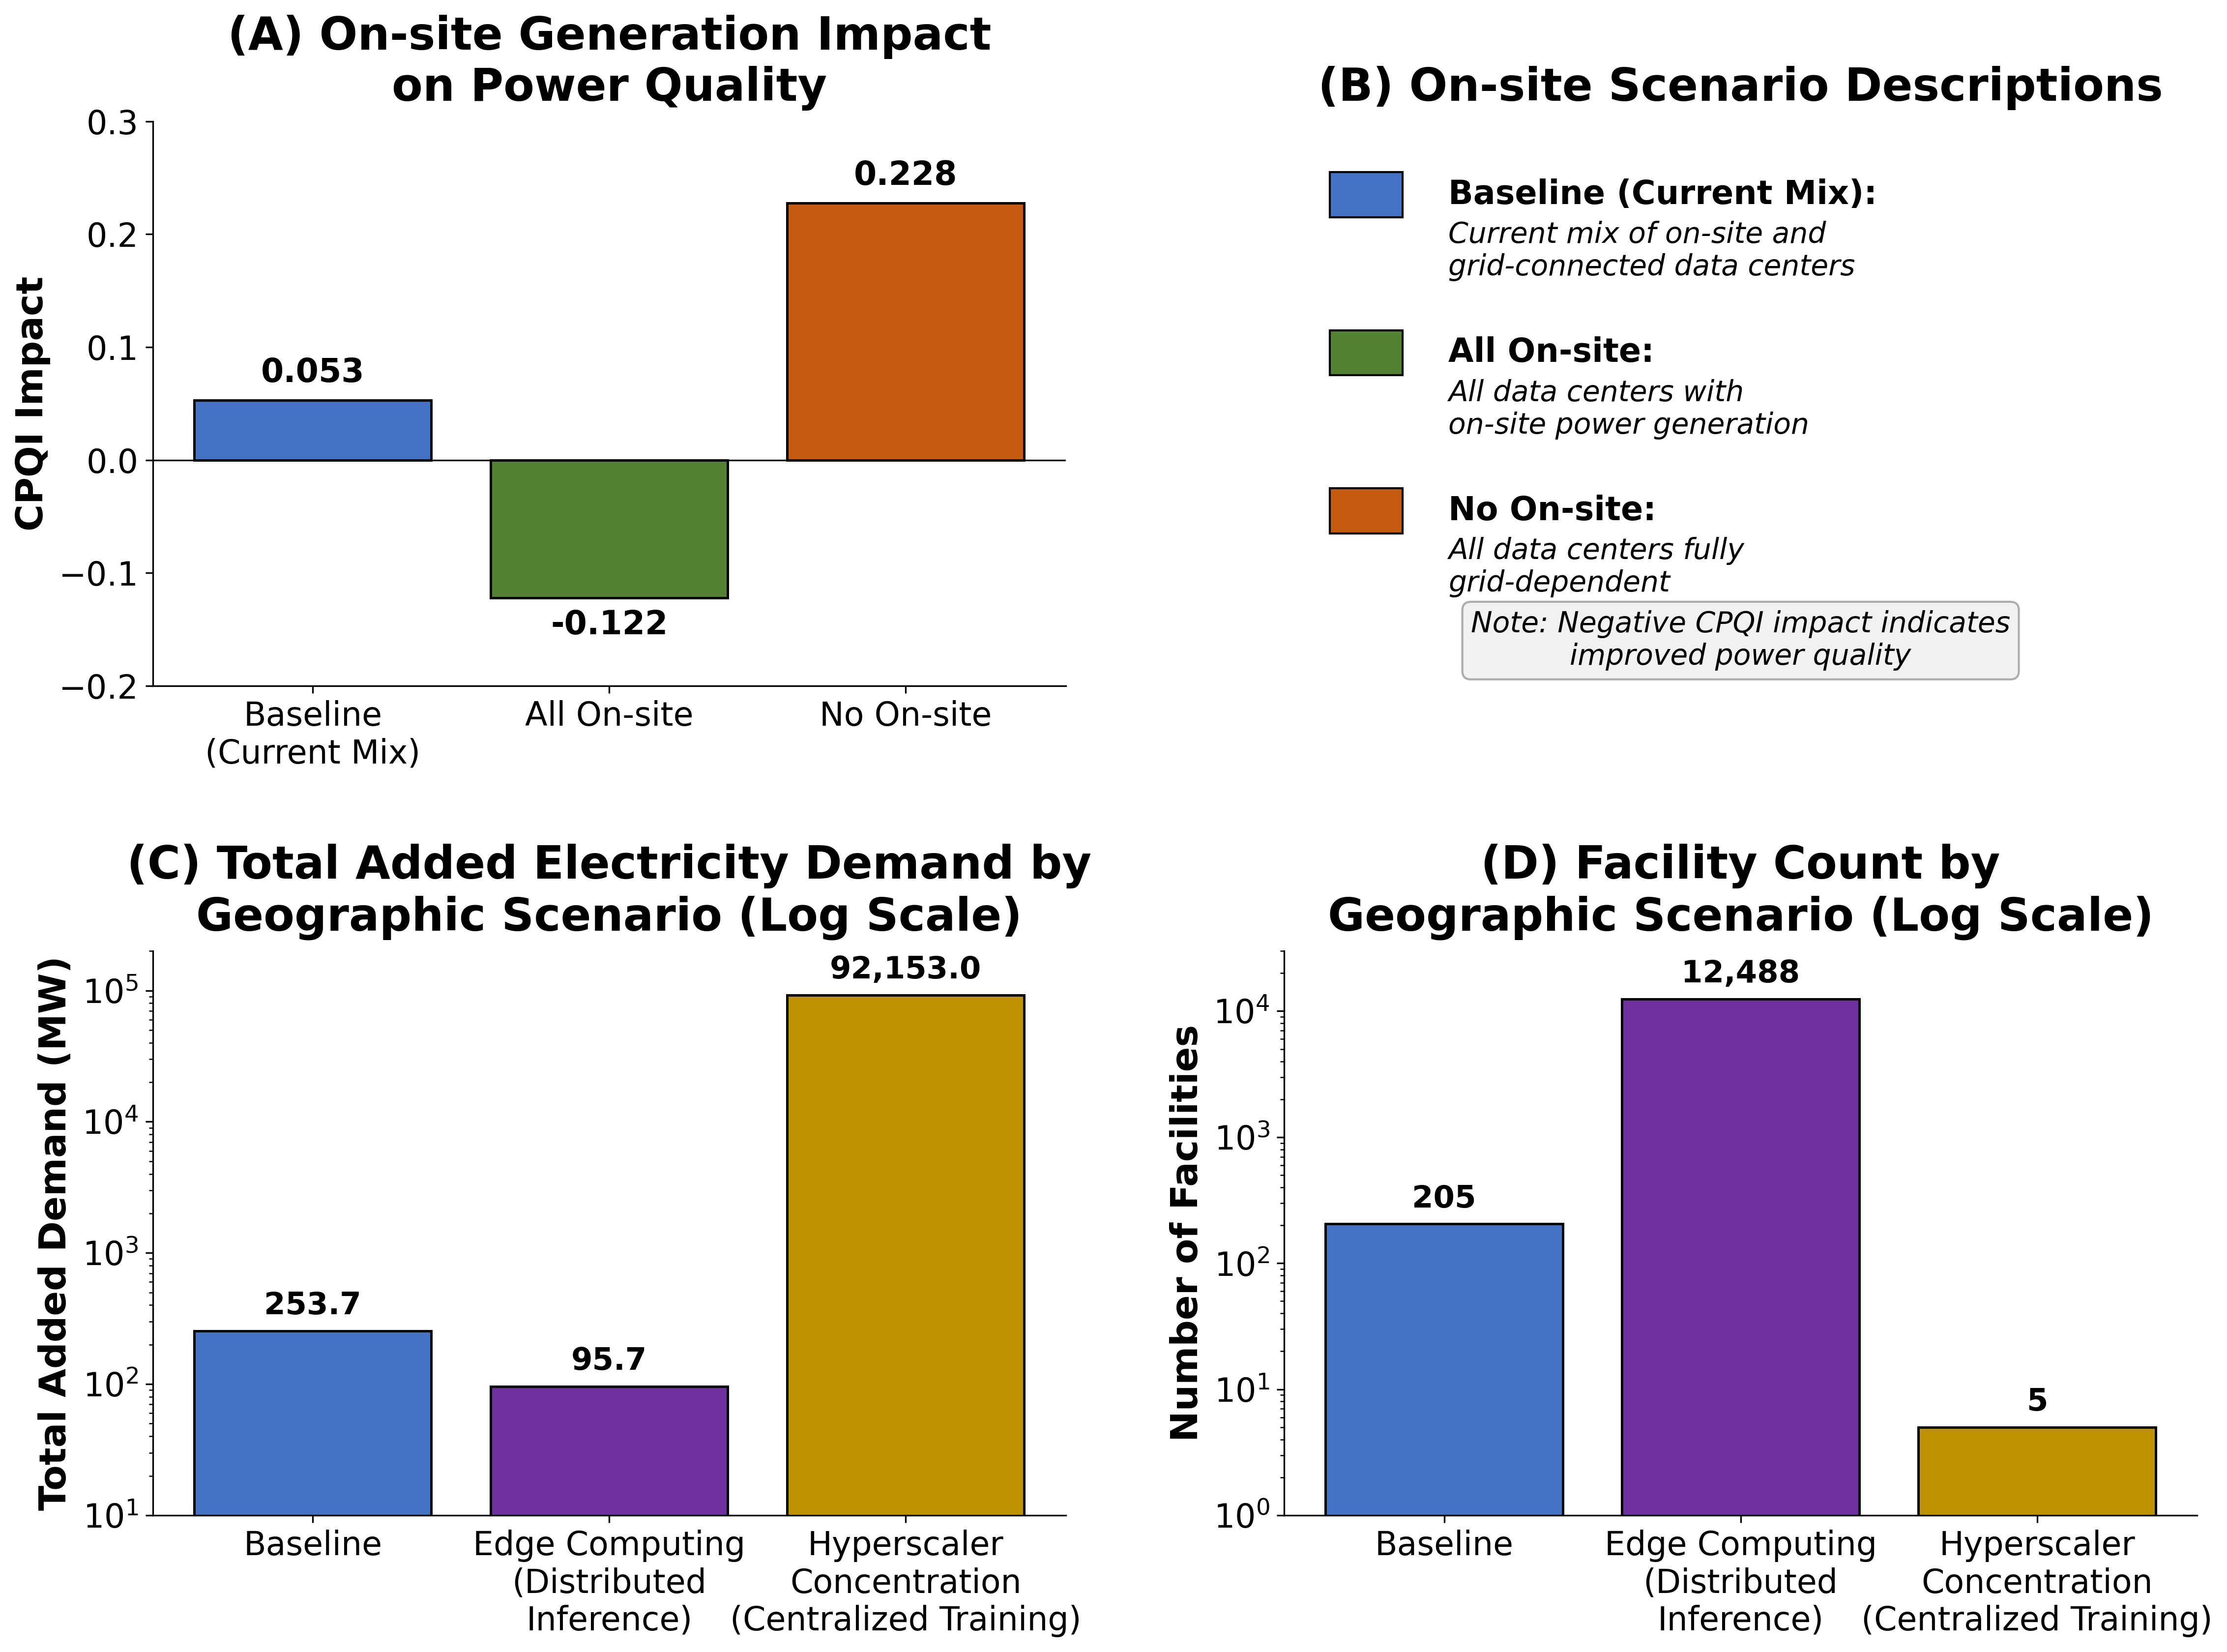
\includegraphics[width=.9\linewidth]{Figures/combined_analysis_figure.png}
    \caption{Effects of Geographic Concentration and On-site Generation on AI Impacts on the grid.}
    \label{fig:CounterfactualCombined}
    \vspace{-2em}
\end{figure}

% \subsubsection{Behind-the-Meter Power Generation Scenarios}

% One major question about the evolution of AI infrastructure concerns the role of on-site generation for data centers. To date, on-site generation investments have been relatively limited, but many investments are planned. On-site generation has numerous benefits due to the data center need for continuous direct current power with fast interconnection times and a non-smooth load profile. Significant investments in behind-the-meter power can benefit both the grid and the companies making the investments.

% We consider both a world where behind-the-meter power becomes standard and a world where on-site generation plays no role in data center power. Figure~\ref{fig:btm_scenarios} demonstrates how baseline AI impacts would change under these scenarios. Remarkably, considering only treated observations, universal adoption of BTM power would shift the impact of data centers from a net detriment to power quality to a net improvement. This suggests that data center investment in power generation substantially improves overall grid outcomes.


% \subsubsection{Additional Counterfactuals}

% Other counterfactuals could be performed with our framework, including:
% \begin{itemize}
%     \item Regressing inference coefficients on reported model queries to determine the scaling effect of additional queries on demand.
%     \item Estimating carbon emissions impacts based on the generation mix in affected regions.
%     \item Analyzing how time-of-use pricing or demand response programs might alter the temporal distribution of AI loads and associated grid impacts.
% \end{itemize}
% These extensions are left for future work.

\section{Conclusion}
Understanding how AI models impact U.S. power grids is critical for ensuring energy reliability and security. This work highlights the challenges in quantifying this impact using existing data sources. It introduces a rigorous econometric methodology to overcome the lack of fine-grained data about contributing factors. In particular, we use difference-in-differences regressions to provide econometric estimates of the amount of power being used by specific AI models as well as the power distortions being caused by AI and the impacts of AI on price. We find evidence that AI is making power quality significantly worse and increasing fossil fuel power demand. Using counterfactual analyses, we provide estimates of the potential impacts of increasing efficiency of AI on the power draw of data centers. We also show how changes in the geographic composition of AI, a potential shift to edge computing, and a shift in the ratio of training to inference conducted impact the power market.
%Understanding how AI models impact U.S. power grids is critical for ensuring energy reliability and security. Our rigorous econometric analyses supported by carefully constructed data enables us to quantify the substantial impacts of AI model training and inference on the power quality, demand, and price in nearby power-grids. 

%The approach we introduce provides more realistic estimates than previous works (\nb{I am worried we dont have direct comparisons to related work, so best to leave this claim out.}



%Understanding how AI models impact U.S. power grids is critical for ensuring energy reliability and security. This work introduces an econometric methodology to overcome the lack of fine-grained data about contributing factors. In particular, we use a difference-in-differences regressions to provide econometric estimates of the amount of power being used by specific AI models as well as the power distortions being caused by AI and the impacts of AI on price. We find evidence that AI is making power quality significantly worse and increasing fossil fuel power demand. We provide estimates of the potential impacts of increasing efficiency of AI on the power draw of data centers. We also show how changes in the geographic composition of AI, a potential shift to edge computing, and a shift in the ratio of training to inference conducted impact the power market.

%Our approach differs from the approach traditionally taken by the computer science energy efficiency literature, which tends to focus on the micro-scale to build up estimates of the costs of training a model in a specified way a specified number of times. Our estimates of power demand impacts are significantly higher than previous literature estimates. We believe this is primarily because we capture lifecycle and indirect power usage effects that most papers miss. Our approach also differs from the current approach amongst energy economists who tend to utilize changes from baseline simulation models to determine the impacts of external demand shocks. By focusing on market data, our approach is able to achieve estimates that are in between these levels of analysis. Our estimation is able to agnostically consider all additional electrical load from AI model activities, which provides a more realistic estimate of AI life-cycle power demand. We believe this approach is also applicable for other other opaque impacts—such as the effect of large model releases on network congestion or cooling water demand—wherever direct usage data from providers is inaccessible.



%Our methodological contribution is portable beyond the specific case of AI and electricity. By combining econometric causal inference (difference-in-differences, instrumental variables) with domain-specific data sources, we establish a general toolkit for quantifying hidden infrastructure externalities of AI systems. The same design could be adapted to study other opaque impacts—such as the effect of large model releases on network congestion, semiconductor supply chains, or cooling water demand—whenever direct usage data from providers are inaccessible. In this sense, our approach provides a scalable, data-efficient way for AI researchers to infer systemic costs and reliability effects, complementing simulation-based analyses in computer science with causal identification strategies from economics.

%\nb{Move this to }
%While informative, this approach inherits the limitations of all Difference-in-Differences experimental designs. It relies on the parallel trends assumption, which may be violated if treated and control regions were already diverging or if generators anticipated model releases. %Spillovers across regions and heterogeneous impacts by grid or model type can further bias estimates.Timing is also critical—effects may emerge gradually or with lags, complicating interpretation. Finally, contemporaneous shocks such as weather or other industrial expansions can confound results, and the treatment itself (a model release) may not map cleanly onto actual deployment. Ideally, we would like a longer power quality dataset with more granularity to make cleaner statements about long-term trends.

\bibliography{Energy}

\newpage

\appendix
\section{Appendix}
\subsection{Total Harmonic Distortion}
\begin{wrapfigure}{r}{0.3\linewidth}
    \centering
    \vspace{-18pt}
    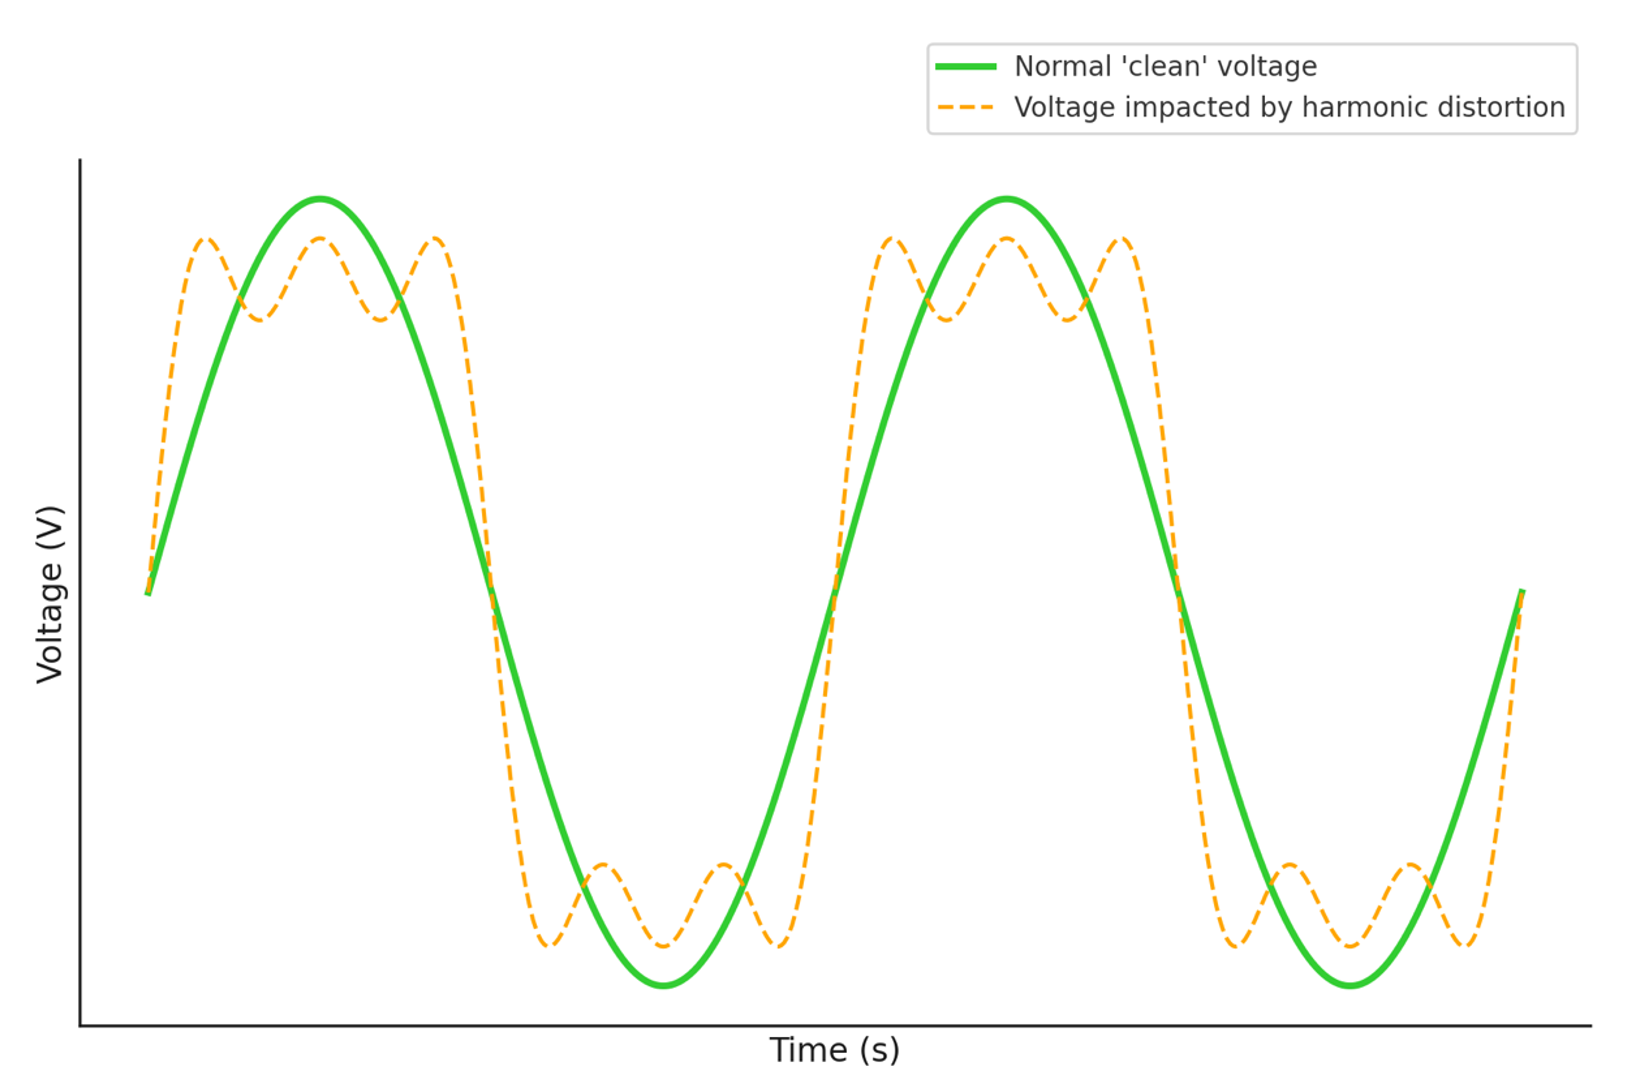
\includegraphics[width=\linewidth]{Figures/HarmonicDistortion.png}
    \caption{Total harmonic distortion representation.}%\aruna{this figure is not referenced in the text}}        
    \label{fig:THD}
    \vspace{5pt}
\end{wrapfigure}
Figure~\ref{fig:THD} illustrates the distortions in the power frequencies. The green lie shows the \emph{clear} voltage curve, which is cleanly sinusoidal, whereas with huge loads can produce harmonic distortions shown as the dotted yellow curve. This \emph{dirtier} voltage can adversely affect the operation and lifetime of household appliances and other products that use electricity.

\subsection{Expanded Dataset Description}

Below, maps can be found providing more detail on the data center dataset alongside tables on the datasets and the dataset sample selection criteria.

\begin{figure}[h]
    \centering
    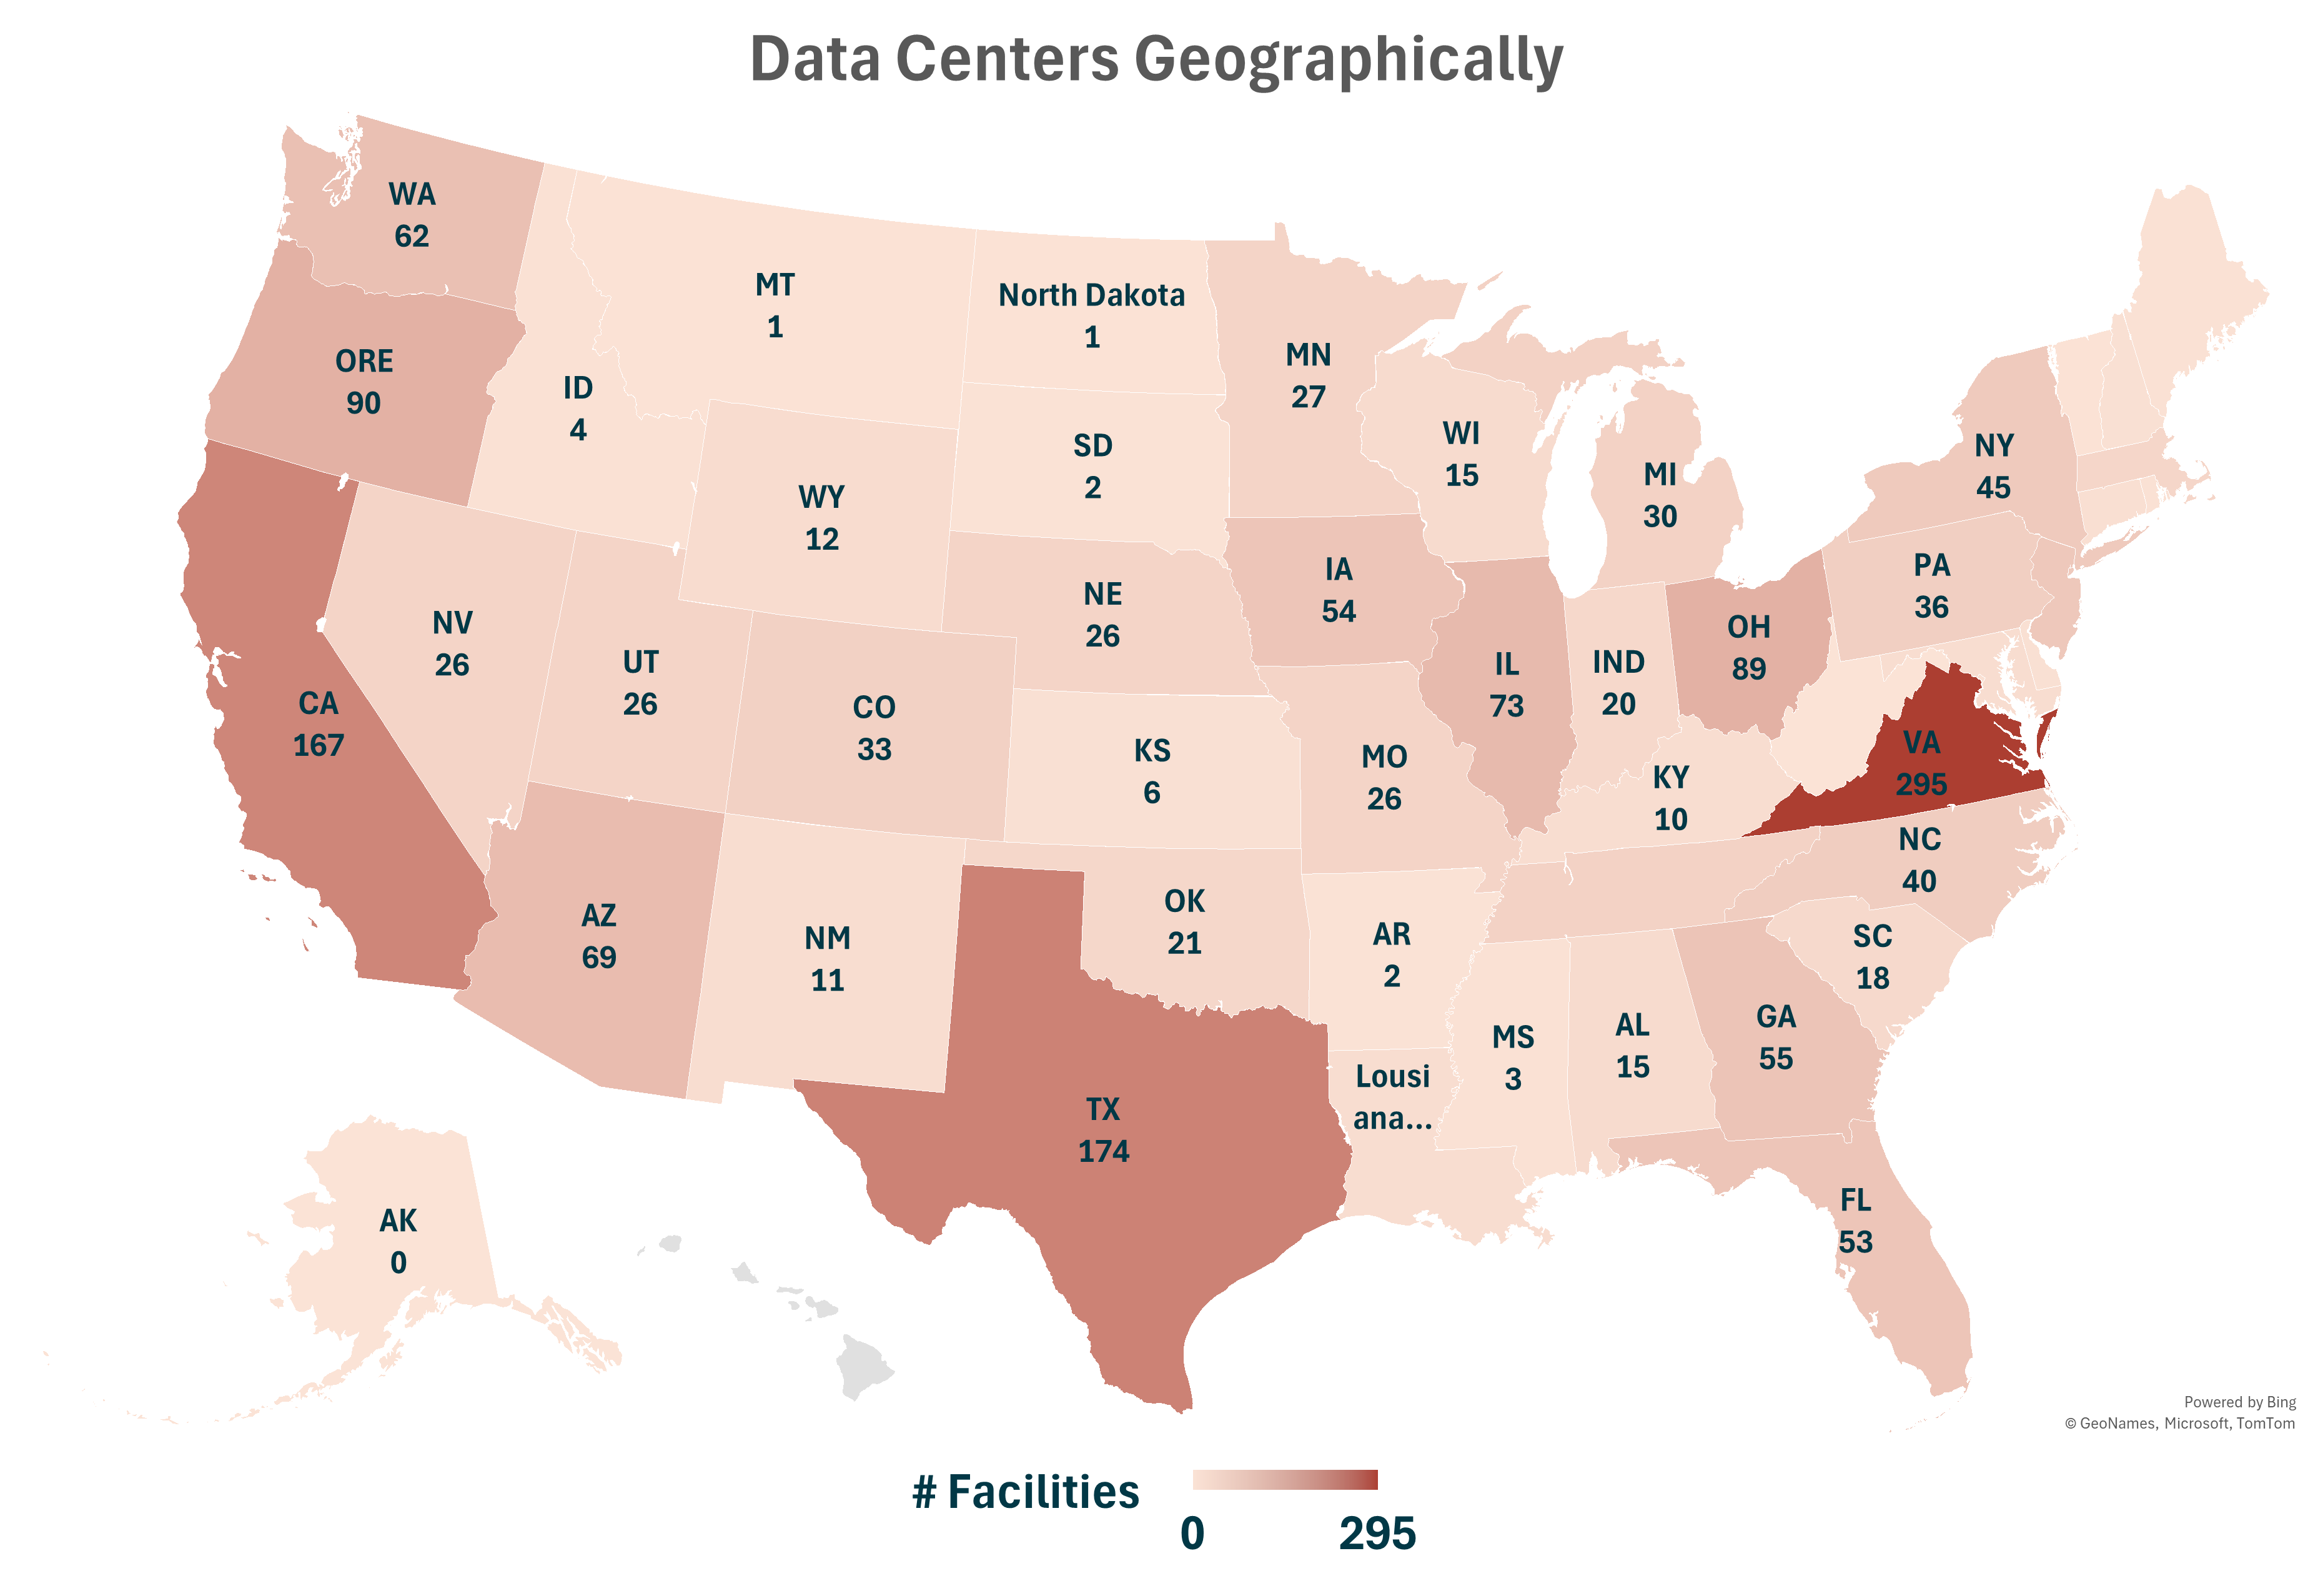
\includegraphics[width=\linewidth]{Figures/Data Centers by State.png}
    \caption{Data centers by state.}
    \label{fig:placeholder}
\end{figure}

\begin{figure}[h]
    \centering
    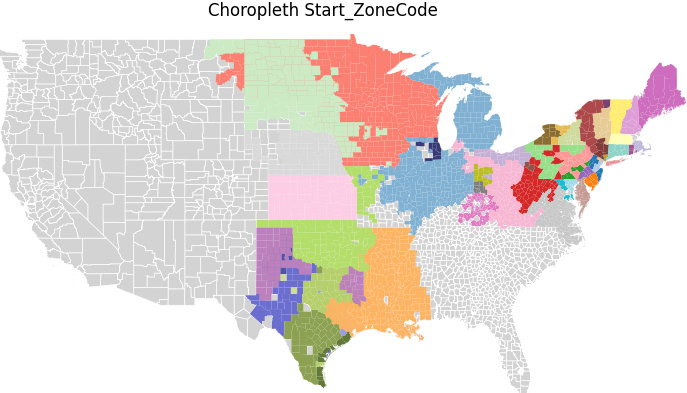
\includegraphics[width=\linewidth]{Figures/ZoneMap (1).png}
    \caption{Map of zones for demand model.}
    \label{fig:MapofZonesRegular}
\end{figure}

\begin{figure}[h]
    \centering
    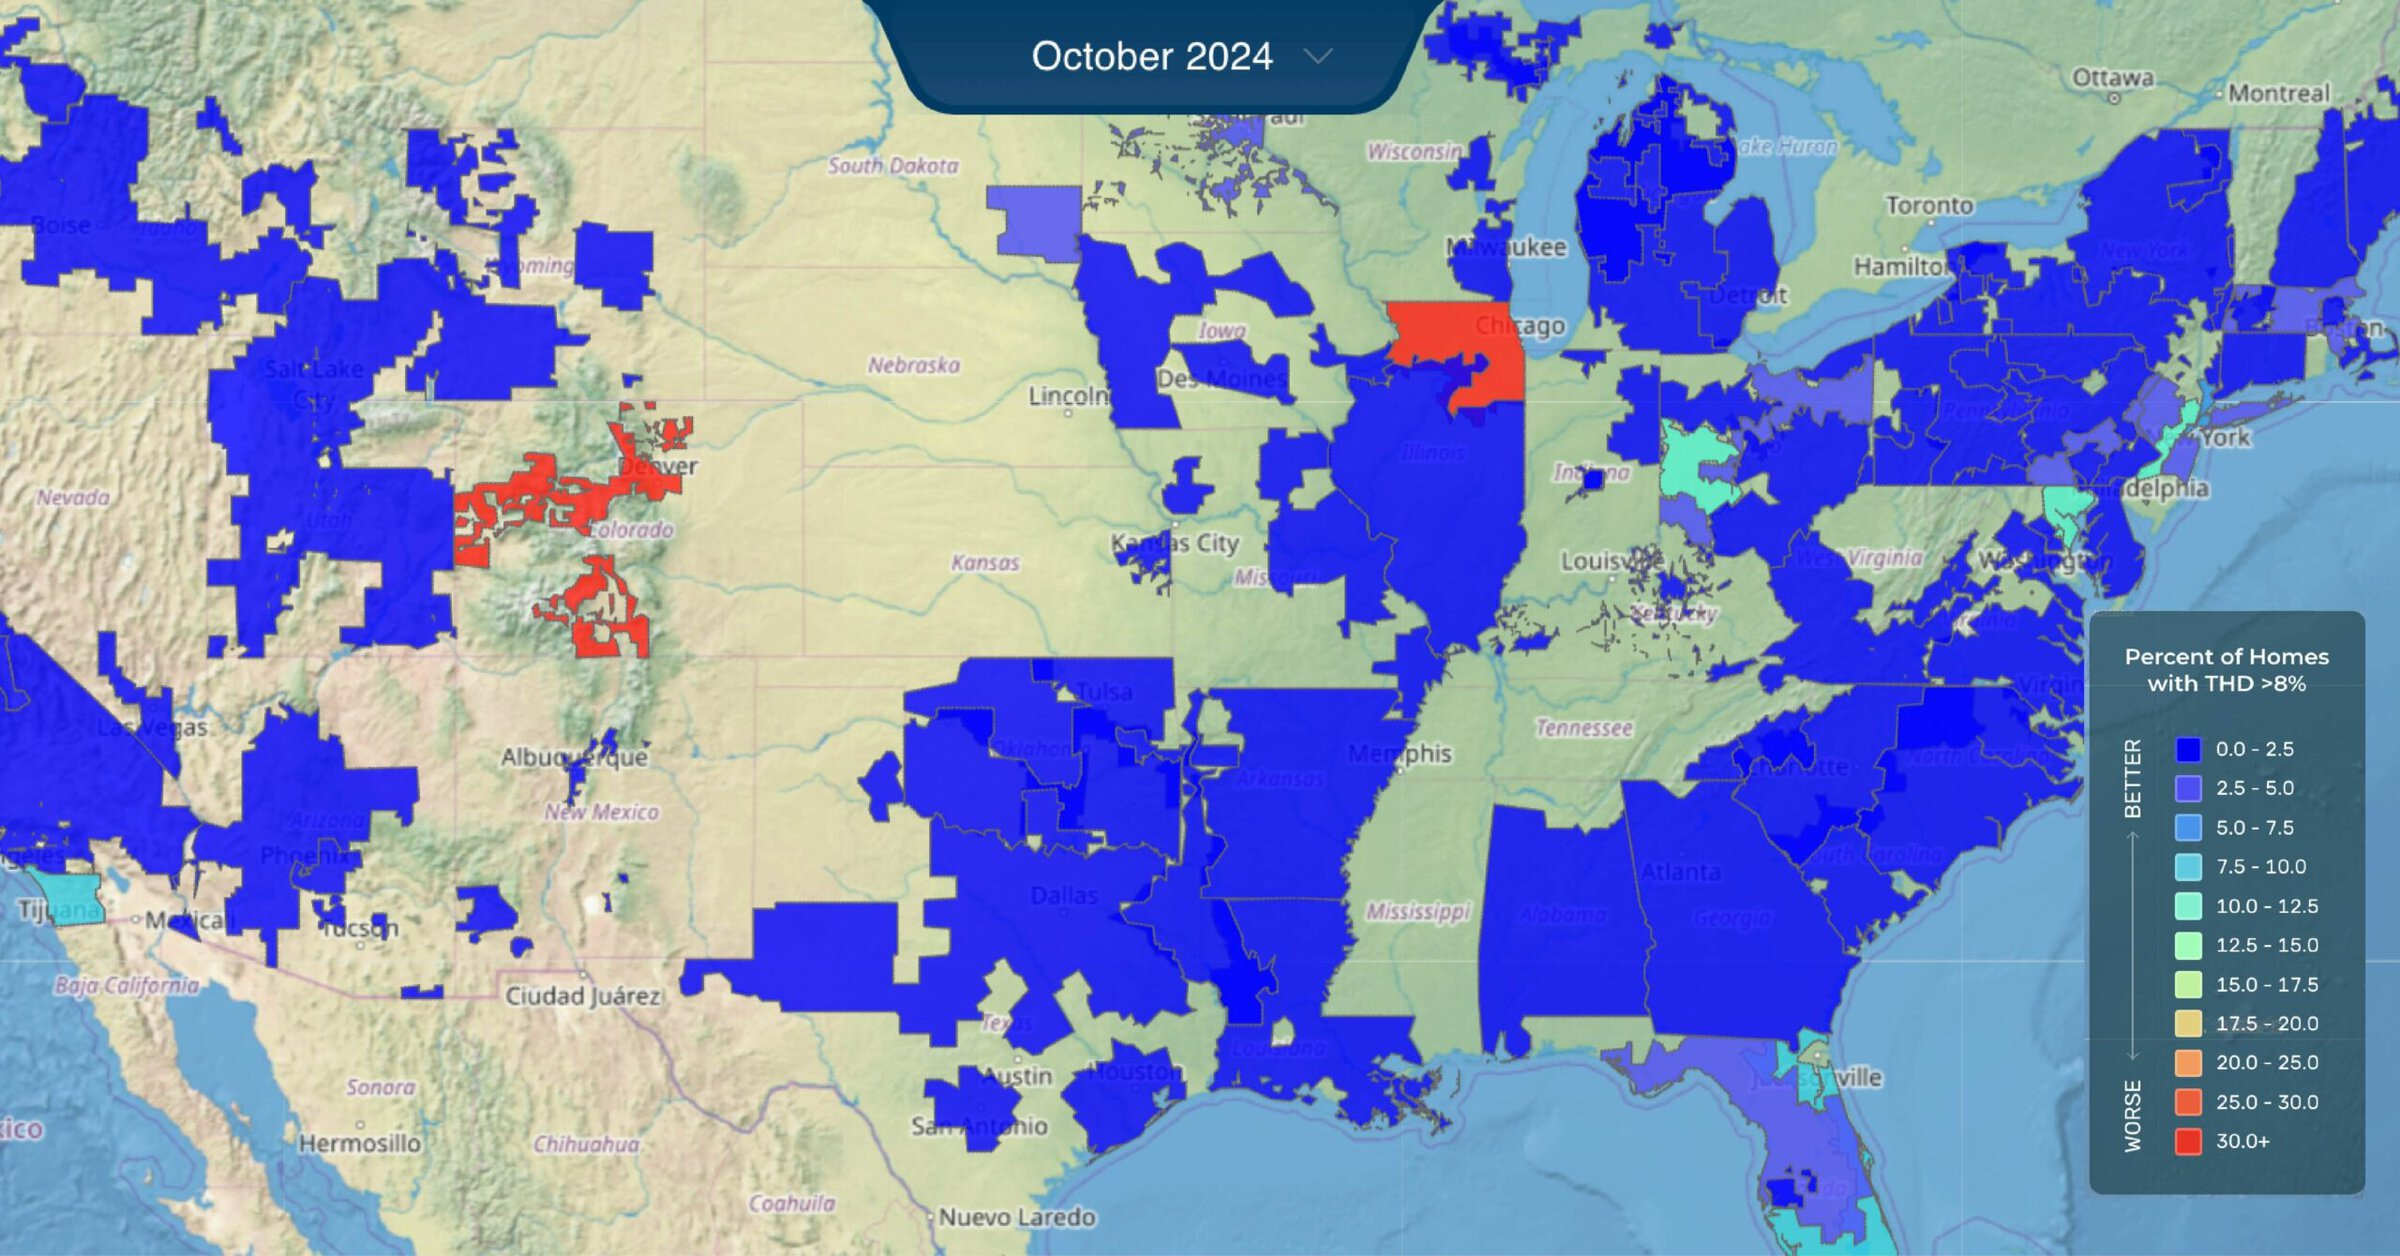
\includegraphics[width=\linewidth]{Figures/THD Dataset.jpg}
    \caption{Map of Retail Electric Utilities for Whisker Labs Data.}
    \label{fig:placeholder}
\end{figure}

\begin{figure}
    \centering
    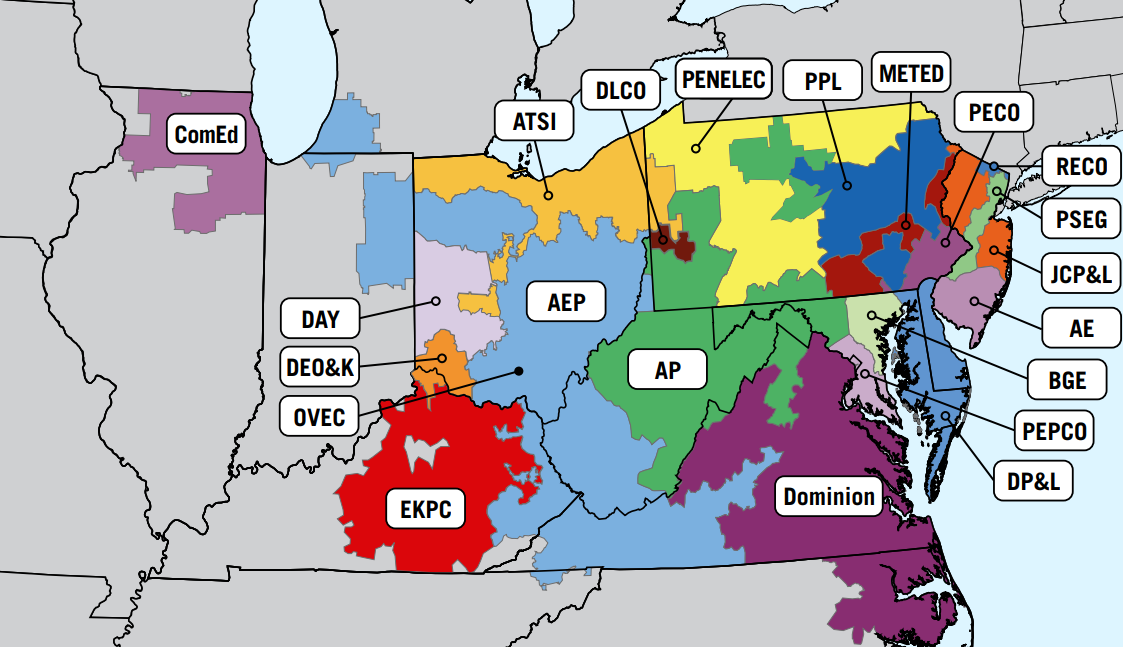
\includegraphics[width=0.75\linewidth]{Figures/PJMZonalMap.png}
    \caption{Map of PJM by Zones.}
    \label{fig:placeholder}
\end{figure}

\newpage
\clearpage
\begin{sidewaystable}[p]
\centering
\caption{Expanded description of data sources (for appendix).}
\label{tab:DataSourcesExpanded}

\begin{adjustbox}{max width=\textheight} % <-- key: rotated page's usable width
\begin{threeparttable}
\begin{tabular}{p{0.18\textheight} p{0.55\textheight} p{0.25\textheight}}
\toprule
\textbf{Source} & \textbf{Content and Granularity} & \textbf{Use in Analysis} \\
\midrule
\multicolumn{3}{c}{\textbf{Q1: Difference-in-Differences (Power Quality)}} \\
\midrule
Aterio & Data center locations, establishment/expansion/retirement dates, ownership, and operational capacity (MW). Data are available at the facility level and updated annually. & Defines treatment regions; links AI model releases to hyperscaler-owned centers. \\
Whisker Labs & Consumer Power Quality Index (CPQI, composite measure of surges, sags, brownouts, interruptions) and Total Harmonic Distortion (THD, waveform distortion). Provided at county level, hourly frequency. & Outcome variables for DiD regressions. \\
Meteostat & Hourly temperature and precipitation, aggregated at the county level. Coverage includes all U.S. counties with weather stations. & Controls for demand fluctuations and renewable generation variability. \\
ISOs & Geographic boundary shapefiles and wholesale price data at zonal level. Boundaries digitized from ISO-provided maps; prices available hourly. & Market alignment and regional controls. \\
EIA & Retail service territory shapefiles, at utility level, updated periodically. & Used to define treatment/control boundaries and reconcile geographies. \\
\midrule
\multicolumn{3}{c}{\textbf{Q2: Instrumental Variables (Fossil Demand)}} \\
\midrule
EPA CAMPD & Hourly generator-level demand (MWh) and unit-specific heat rates (Btu/kWh). Coverage 2021--2023. & Generator demand is outcome; heat rates serve as instruments for prices. \\
S\&P Capital IQ & Daily natural gas price series, Henry Hub benchmark. National coverage. & Instrument for price and fuel-cost control. \\
Aterio & Generator proximity to data centers owned by releasing companies, matched at 20-mile radius. & Defines treatment generators in IV design. \\
Meteostat & Hourly temperature and precipitation, as above. & Controls for demand and renewable variability. \\
ISOs & Wholesale price series, zonal level, hourly frequency. & Market-level controls. \\
\midrule
\multicolumn{3}{c}{\textbf{Q3: Counterfactual Analyses (Scaling, Efficiency,  \& Tech Development)}} \\
\midrule
Whisker Labs & CPQI and THD (as above). Used to establish baseline deterioration in power quality. & Benchmark outcomes for scaling projections. \\
Epoch & AI model metadata: release dates, FLOPs, parameter counts. Public dataset with model-level detail. & Used for scaling regressions and efficiency counterfactuals. \\
GPU Experiments & Energy use measured on NVIDIA A6000 GPUs. Experiments run with batch size 4, sequence length 1024, and 200 inferences. Each bar in results represents total energy; lighter portion indicates communication overhead. Data collected in-house on 8xA6000 cluster. & Provides empirical GPU energy baselines for counterfactual scaling exercises. \\
\bottomrule
\end{tabular}
\end{threeparttable}
\end{adjustbox}
\end{sidewaystable}
\clearpage

\newpage
\clearpage

% 1. These two lines force the sidewaystable to center vertically on the page
\setlength{\rotFPtop}{0pt plus 1fil}
\setlength{\rotFPbot}{0pt plus 1fil}

\begin{sidewaystable}[p] % [p] forces it to be on its own page
\centering
\setlength{\tabcolsep}{3pt}
\renewcommand{\arraystretch}{0.95}

\caption{Dataset sample selection and summary statistics}
\label{tab:SampleSelection}

\begin{threeparttable}
\footnotesize
% 2. Use \linewidth so it fills the text block, but relies on margins for centering
\begin{tabularx}{\linewidth}{lXl} 
\toprule
\textbf{Dataset} & \textbf{Content / Summary Statistics} & \textbf{Sample Selection} \\
\midrule
Aterio & Data center locations, ownership, and capacity; mapped to ISO zones, EIA service territories, and counties & Hyperscaler data centers (Meta, Microsoft, Amazon, Google; Anthropic via Google) \\
\midrule
Whisker Labs & Reliability measures: CPQI ($N=2{,}683$, mean=0.52, s.d.=0.42); THD (mean=1.81, s.d.=6.77) & 72 retail electric utilities, monthly data 2022--2025 \\
\midrule
CAMPD & Generator-level demand: mean 218 MW (s.d.=158); operating times $\approx 1$ & Several thousand fossil generators, hourly data 2021--2023 \\
\midrule
ISOs & Wholesale electricity prices: mean $\$51$/MWh (s.d.=148); zonal boundaries & Deregulated markets in Eastern Interconnection and ERCOT \\
\midrule
Weather (Meteostat) & Temperature (mean=17°C, s.d.=11.4); precipitation (mean=0.12 mm, s.d.=0.91) & Matched by county/zone, hourly or daily resolution \\
\midrule
External Controls & Natural gas prices, ISO market data, geography/time harmonization & Used for both DiD and IV regressions \\
\bottomrule
\end{tabularx}

\begin{tablenotes}
\scriptsize
\item Notes: Time series are harmonized at hourly or monthly resolution depending on source. Unified panel supports both difference-in-differences (power quality) and instrumental variable (demand) regressions. Maps of sample regions provided in the appendix.
\end{tablenotes}
\end{threeparttable}

\end{sidewaystable}
\clearpage
\newpage

\subsection{Dataset Creation Diagram}

\begin{figure}[htbp]
\centering
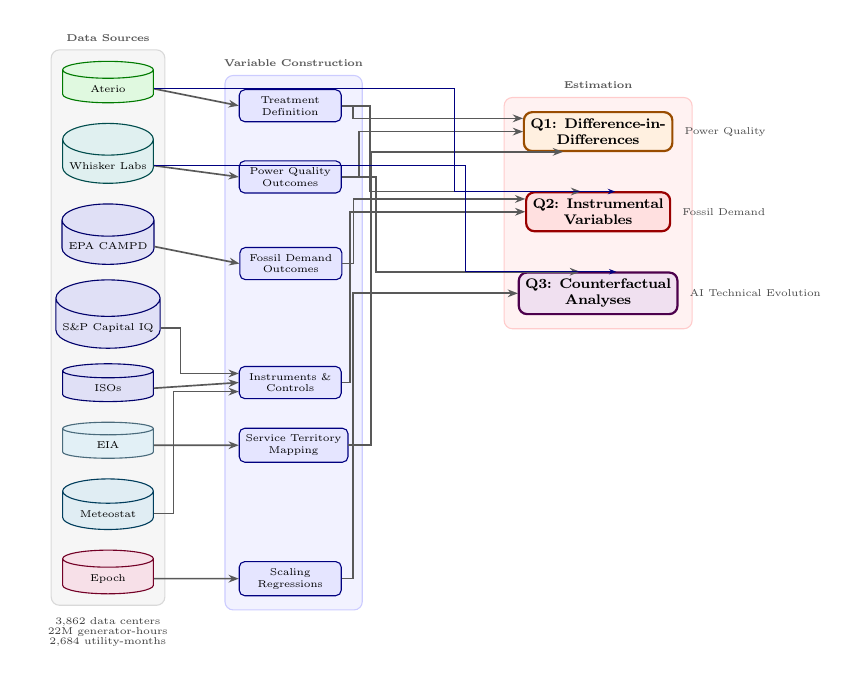
\begin{tikzpicture}[
    scale=0.72,
    transform shape,
    node distance=0.48cm and 0.7cm,
    % === STYLES ===
    source/.style={
        cylinder,
        shape border rotate=90,
        draw=#1!60!black,
        fill=#1!12,
        text centered,
        minimum height=1.55em,
        minimum width=1.6cm,
        aspect=0.35,
        font=\tiny,
        align=center
    },
    source/.default=green,
    process/.style={
        rectangle,
        draw=blue!50!black,
        fill=blue!10,
        text centered,
        rounded corners=2pt,
        minimum height=1.35em,
        minimum width=1.8cm,
        font=\tiny,
        align=center
    },
    model/.style={
        rectangle,
        draw=#1!60!black,
        fill=#1!12,
        thick,
        text centered,
        rounded corners=3pt,
        minimum height=1.85em,
        minimum width=2.4cm,
        font=\scriptsize\bfseries,
        align=center
    },
    model/.default=red,
    arrow/.style={
        -{Stealth[scale=0.65]},
        semithick,
        color=gray!70!black
    },
    directarrow/.style={
        -{Stealth[scale=0.55]},
        color=blue!50!black,
        thin
    },
    grouplabel/.style={
        font=\tiny\bfseries,
        color=gray!70!black
    },
    annot/.style={
        font=\scriptsize,
        color=gray!60!black
    }
]

% === COLUMN 1: DATA SOURCES ===

% AI/Data Center Data (green shades)
\node[source=green!80!black] (aterio) {Aterio};

% Power Quality Data (teal shades)
\node[source=teal, below=0.35cm of aterio] (whisker) {Whisker Labs};

% Generator/Market Data (blue shades)
\node[source=blue!70!black, below=0.35cm of whisker] (campd) {EPA CAMPD};
\node[source=blue!70!black, below=0.26cm of campd] (spiq) {S\&P Capital IQ};
\node[source=blue!70!black, below=0.26cm of spiq] (isos) {ISOs};

% Government/Geographic (cyan shades)
\node[source=cyan!70!black, below=0.35cm of isos] (eia) {EIA};

% Weather (blue-green shades)
\node[source=blue!60!green, below=0.35cm of eia] (weather) {Meteostat};

% AI Model Data (purple shades)
\node[source=purple, below=0.35cm of weather] (epoch) {Epoch};

% === COLUMN 2: DATA CONSTRUCTION STEPS ===

% Treatment Definition
\node[process, right=1.5cm of aterio, yshift=-0.3cm] (treat_def) {Treatment\\Definition};

% Outcome Construction
\node[process, right=1.5cm of whisker, yshift=-0.2cm] (outcome_pq) {Power Quality\\Outcomes};

% Fossil Demand Construction
\node[process, right=1.5cm of campd, yshift=-0.3cm] (fossil_dem) {Fossil Demand\\Outcomes};

% Instrument Construction
\node[process, right=1.5cm of isos, yshift=0.1cm] (instruments) {Instruments \&\\Controls};

% Service Territory Mapping
\node[process, right=1.5cm of eia] (territory) {Service Territory\\Mapping};

% Scaling Data
\node[process, right=1.5cm of epoch] (scaling) {Scaling\\Regressions};

% === COLUMN 3: ANALYSIS MODELS ===

% Q1: DiD Model
\node[model=orange, right=3.2cm of outcome_pq, yshift=0.8cm] (q1) {Q1: Difference-in-\\Differences};

% Q2: IV Model  
\node[model=red, below=0.7cm of q1] (q2) {Q2: Instrumental\\Variables};

% Q3: Counterfactual Model
\node[model=violet, below=0.7cm of q2] (q3) {Q3: Counterfactual\\Analyses};

% === CONNECTIONS ===

% To Treatment Definition
\draw[arrow] (aterio.east) -- (treat_def.west);

% To Power Quality Outcomes
\draw[arrow] (whisker.east) -- (outcome_pq.west);

% To Fossil Demand Outcomes
\draw[arrow] (campd.east) -- (fossil_dem.west);

% To Instruments & Controls
\draw[arrow] (spiq.east) -- ++(0.35,0) |- (instruments.170);
\draw[arrow] (isos.east) -- (instruments.west);
\draw[arrow] (weather.east) -- ++(0.35,0) |- (instruments.190);

% To Service Territory Mapping
\draw[arrow] (eia.east) -- (territory.west);

% To Scaling Regressions
\draw[arrow] (epoch.east) -- (scaling.west);

% === CONNECTIONS TO MODELS ===

% Q1 connections
\draw[arrow] (treat_def.east) -- ++(0.2,0) |- (q1.170);
\draw[arrow] (outcome_pq.east) -- ++(0.3,0) |- (q1.west);
\draw[arrow] (territory.east) -- ++(0.4,0) |- (q1.210);

% Q2 connections
\draw[arrow] (treat_def.east) -- ++(0.5,0) |- (q2.130);
\draw[arrow] (fossil_dem.east) -- ++(0.2,0) |- (q2.170);
\draw[arrow] (instruments.east) -- ++(0.15,0) |- (q2.west);

% Q3 connections
\draw[arrow] (outcome_pq.east) -- ++(0.6,0) |- (q3.130);
\draw[arrow] (scaling.east) -- ++(0.2,0) |- (q3.west);

% Direct data feeds
\draw[directarrow] (aterio.east) -- ++(5.3,0) |- (q2.50);
\draw[directarrow] (whisker.east) -- ++(5.5,0) |- (q3.50);

% === BACKGROUND GROUPINGS ===
\begin{scope}[on background layer]
    % Raw Data Sources
    \node[fit=(aterio)(epoch), 
          fill=gray!7, 
          rounded corners=3pt, 
          draw=gray!30,
          inner sep=4pt] (rawbox) {};
    \node[grouplabel, above=0.02cm of rawbox.north] {Data Sources};
    
    % Data Construction
    \node[fit=(treat_def)(scaling)(territory)(instruments), 
          fill=blue!5, 
          rounded corners=3pt, 
          draw=blue!20,
          inner sep=5pt] (constructbox) {};
    \node[grouplabel, above=0.02cm of constructbox.north] {Variable Construction};
    
    % Models
    \node[fit=(q1)(q2)(q3), 
          fill=red!5, 
          rounded corners=3pt, 
          draw=red!20,
          inner sep=5pt] (modelbox) {};
    \node[grouplabel, above=0.02cm of modelbox.north] {Estimation};
\end{scope}

% === ANNOTATIONS ===
% Observation counts
\node[font=\fontsize{4}{5}\selectfont, color=gray!50!black, below=0.08cm of rawbox.south, text width=2.6cm, align=center] 
    {3,862 data centers\\22M generator-hours\\2,684 utility-months};

% Model annotations
\node[annot, right=0.08cm of q1.east] {\tiny Power Quality};
\node[annot, right=0.08cm of q2.east] {\tiny Fossil Demand};
\node[annot, right=0.08cm of q3.east] {\tiny AI Technical Evolution};

\end{tikzpicture}
\caption{Data sources and analysis pipeline. Data sources flow through variable construction into three estimation strategies addressing power quality impacts (Q1), fossil fuel demand (Q2), and counterfactual scaling scenarios (Q3).}
\label{fig:DataDiagram}
\end{figure}

\subsection{Calculation of Comparisons}

We calculate the household average energy usage based on data provided by \cite{USHouseholdConsumption}. We simply divide our estimates by the provided numbers to get the number of households for our comparisons.

\newpage

\subsection{Specifically Verified Models}
\label{appendix:verified-models}
Below is a subset of our dataset for specifically verified models to provide an example of the data:

\begin{table}[htbp]
\centering
\caption{Documented Training Locations (All Confirmed)}
\label{tab:training_locations}
\small
\begin{tabular}{@{}lll@{}}
\toprule
Model & Location & Source \\
\midrule
GPT-4 & W. Des Moines, IA & \cite{smith2023iowa} \\
PaLM, LaMDA, MUM & Mayes County, OK & \cite{googlecloud2023mlhub} \\
Megatron-Turing NLG & Santa Clara, CA & \cite{nvidia2021megatron} \\
\bottomrule
\end{tabular}
\end{table}

\begin{table}[htbp]
\centering
\caption{Verified Model Dates}
\label{tab:verified_model_dates}
\small
\begin{tabular}{@{}llll@{}}
\toprule
Model & Type & Date & Source \\
\midrule
GPT-3 & API & 2021-11-18 & \cite{openai_api_nowaitlist_2021} \\
Claude 2.1 & API & 2023-11-21 & \cite{anthropic_claude2_1_2023} \\
PaLM API & API & 2023-03-14 & \cite{google_palm_api_makersuite_2023} \\
Llama 2 & API & 2023-07-18 & \cite{meta_llama2_2023} \\
Code Llama & Train & 2023-01--07\textsuperscript{*} & \cite{meta_code_llama_paper_2023} \\
\bottomrule
\multicolumn{4}{@{}l@{}}{\footnotesize \textsuperscript{*}Date range (month precision)} \\
\end{tabular}
\end{table}

\subsection{PJM price Elasticities}\label{PriceElasticityAppendix}

\begin{figure}[H]
    \centering
    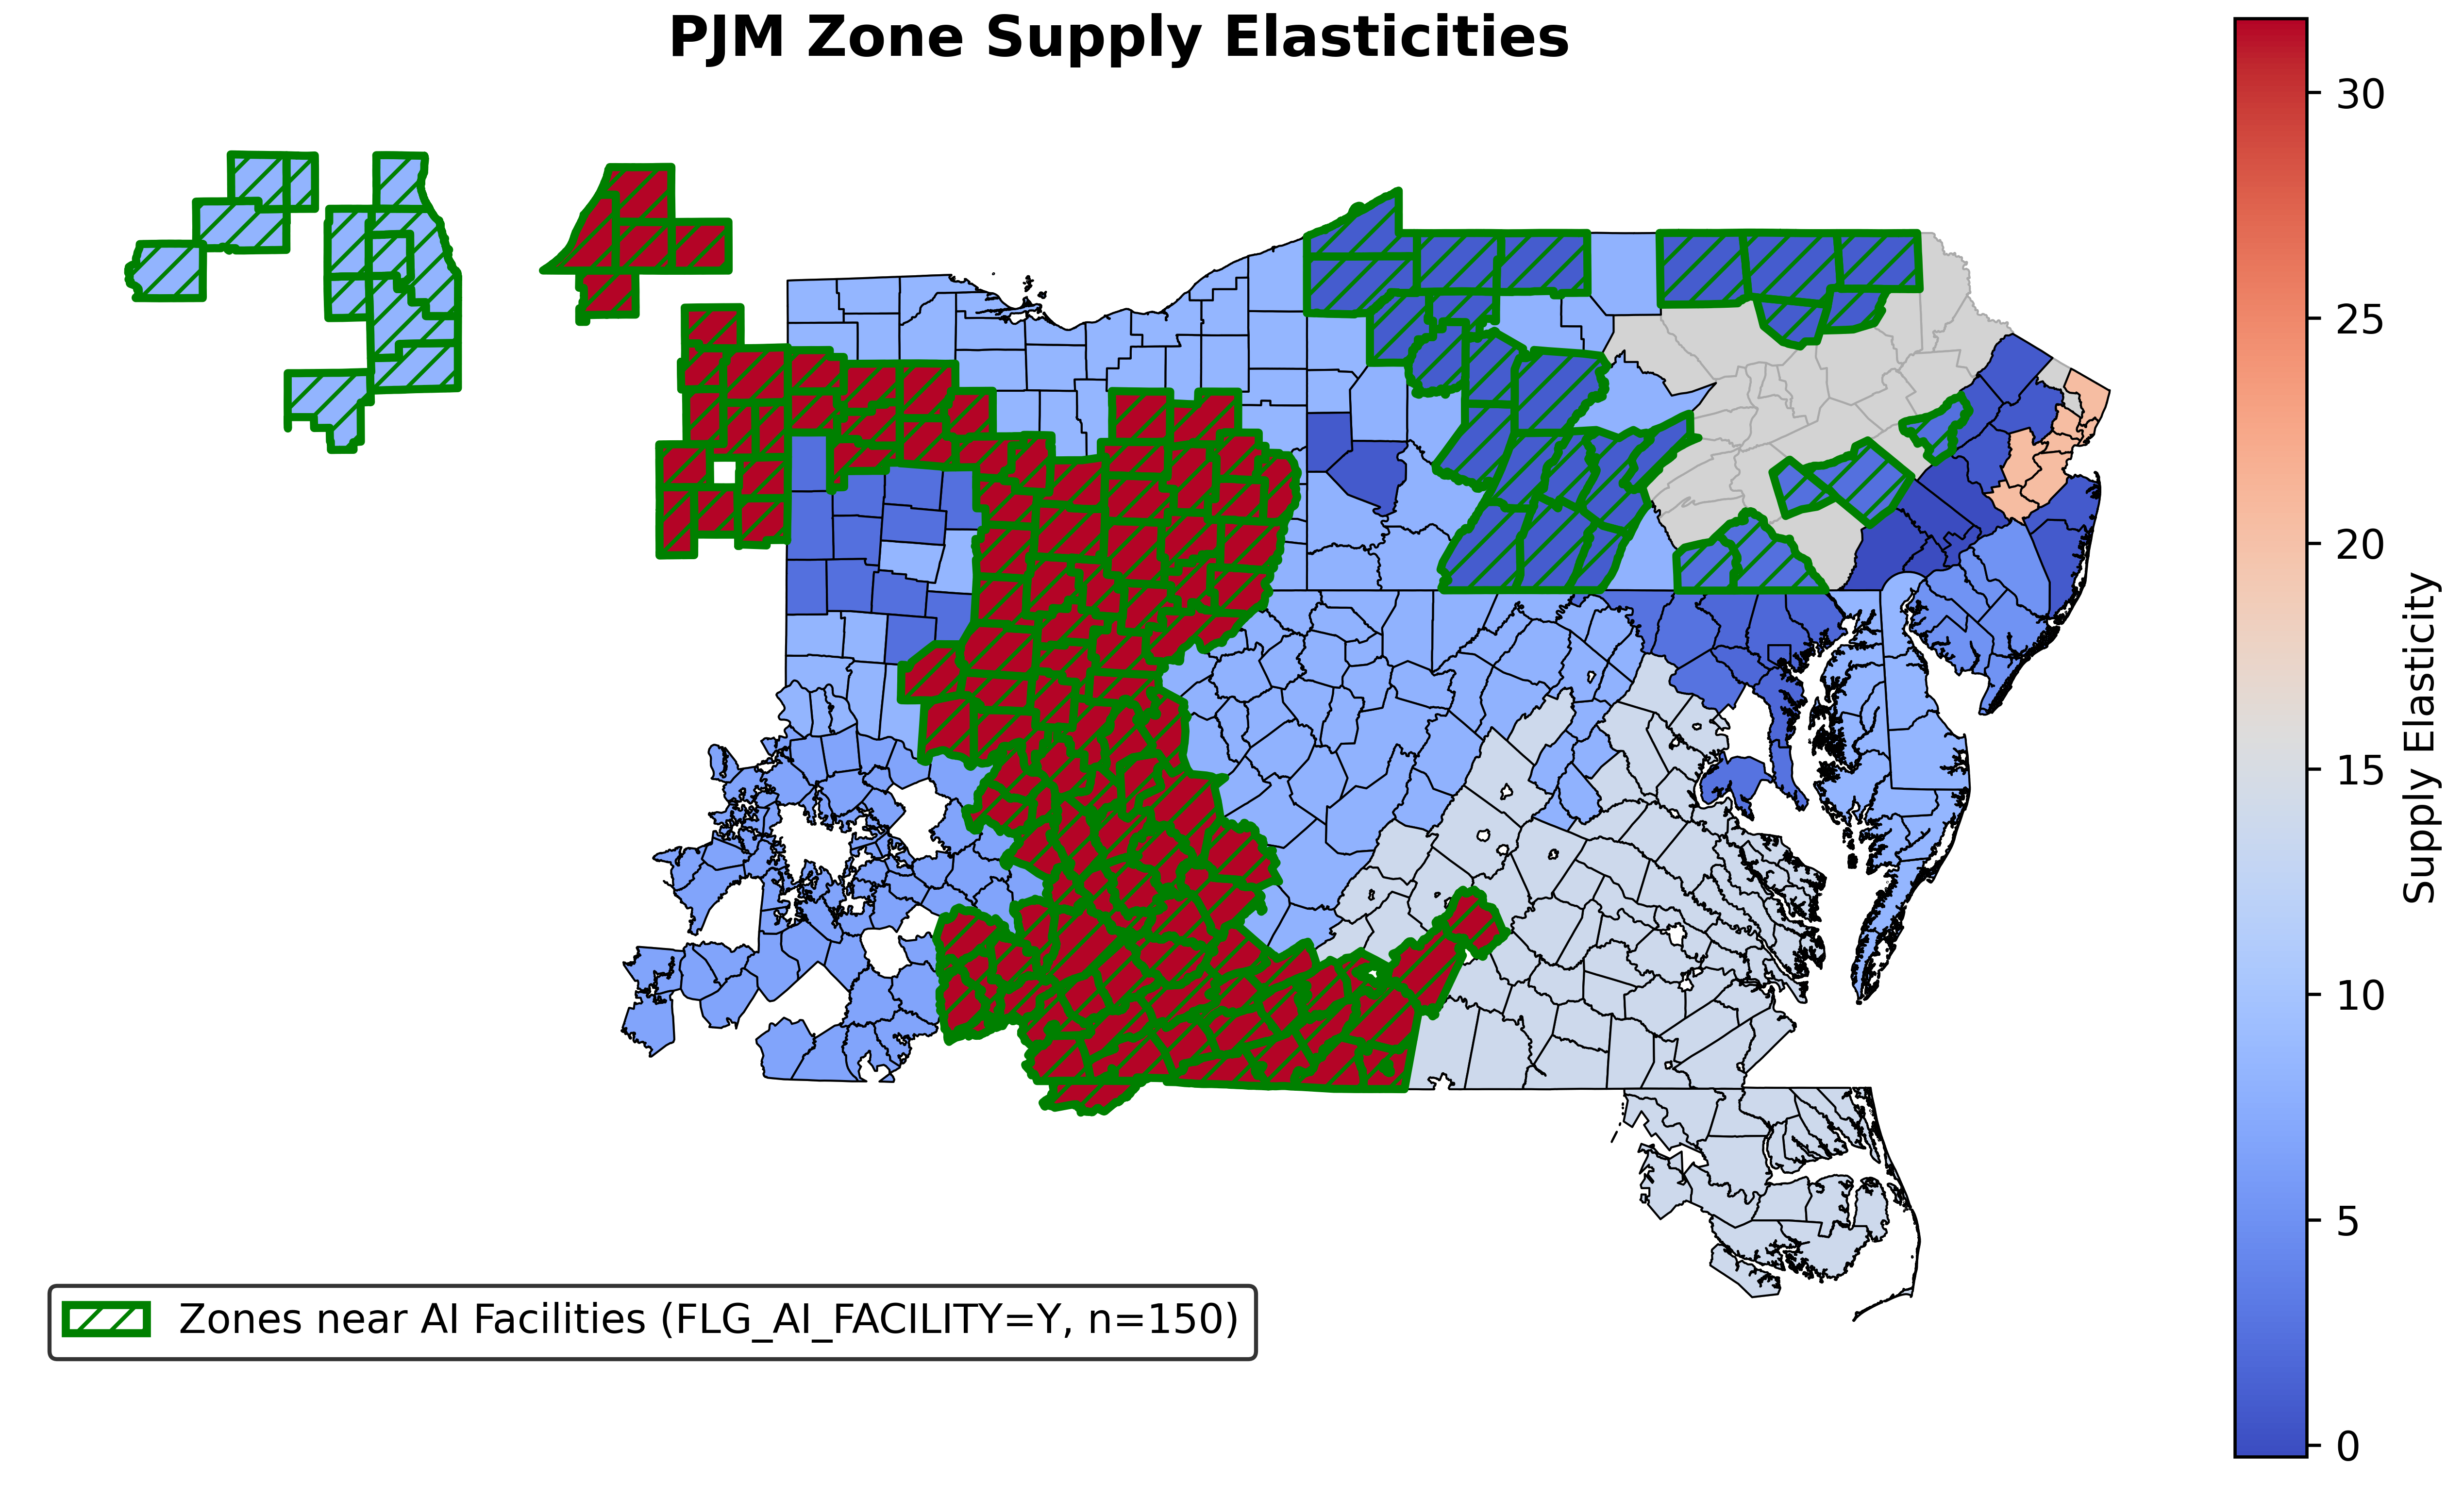
\includegraphics[width=0.5\linewidth]{Figures/pjm_ai_supply Elasticities.png}
    \caption{PJM Price Elasticity by Zone}
    \label{PJMPRiceElasticity}
\end{figure}

\subsection{Treatment Definition and Data Linkage}
\label{subsec:treatment}

Our treatment relies on linking AI model releases to geographic regions through a chain of observable connections: models to companies, companies to data center locations, and data center locations to electricity service territories. We describe each link and its limitations.

\subsubsection{Identifying AI Data Centers}

We leverage a recently released variable from Aterio that directly classifies data centers by their primary use case, including a designation for AI-focused facilities. This classification improves upon prior approaches that treated all data centers homogeneously, as AI workloads---particularly large-scale model training---exhibit distinct load profiles characterized by sustained high utilization and substantial power draws that differ markedly from traditional cloud computing or storage operations.

We link data centers to electricity service territories at two geographic resolutions:
\begin{itemize}
    \item \textbf{Utility service territory:} For power quality analysis, we match AI data centers to retail electric utility boundaries. A utility is designated as treated if at least one AI data center operates within its service territory.
    \item \textbf{Generator proximity:} For fossil fuel demand analysis, we match data centers to generators by picking generators within a 20-mile radius of an in-sample data center. This finer resolution exploits the greater spatial granularity of EPA generator-level data.
\end{itemize}

\subsubsection{Linking Models to Data Centers}

We construct a crosswalk from AI model releases to data center locations through company ownership. For each major model release in our sample, we identify the developing company and link to all AI-classified data centers operated by or contracted to that company. 

\paragraph{Identifying Assumption and Limitations.} Our approach assumes that training and inference activity for a given model occurs at data centers associated with the releasing company. This assumption is imperfect for several reasons:
\begin{enumerate}
    % \item We do not observe the specific facility where training occurred. A company with multiple data centers may concentrate training at a subset of locations.
    \item Training may occur at third-party cloud facilities not captured in our data center inventory.
    \item Inference workloads may be distributed across facilities differently than training workloads.
\end{enumerate}

We interpret our estimates as capturing the \textit{average} effect across a company's AI data center footprint, which represents a lower bound on the localized effect at the actual training site if activity is concentrated, or an upper bound if we misattribute activity to facilities that were not involved. We probe robustness to this measurement error through several approaches described in Section~\ref{subsec:robustness}.

For a subset of models where public information permits more precise dating, we supplement our treatment timing with verified training and inference windows:


\subsubsection{Instrumental Variables Specification}\label{IVDetails}

The learned DiD coefficients capture the relationship between AI model releases and generator output, but this relationship may be confounded by supply-side shocks. For example, if AI model releases coincide with changes in natural gas prices or generator availability that independently affect electricity production, our estimates would conflate demand-side and supply-side effects. To isolate the demand-side effects, we instrument for electricity prices using the interaction of generator-level heat rates and regional natural gas prices. This instrumentation strategy exploits cross-sectional variation in generators' fuel efficiency: conditional on natural gas price movements, generators with higher heat rates (lower efficiency) face larger marginal cost shocks, allowing us to trace out the demand curve.

\paragraph{First-Stage and Structural Estimates.} The first stage regresses electricity prices on the heat rate--gas price interaction. The structural equation then uses predicted prices to estimate price responsiveness. The estimated price elasticity from the structural equation is 0.135 (SE = 0.013, p < 0.0001), indicating economically meaningful and precisely estimated demand responsiveness. As a specification check, we estimate the first stage separately for each of 5 model-specific regressions; the mean price coefficient is $-0.331$ (SD = 0.005, range: $-0.336$ to $-0.323$). The tight clustering of estimates across specifications suggests stable demand elasticity across AI model events and supports the validity of our instrumentation strategy.

\subsection{Wholesale-to-retail Passthrough Estimates}\label{WholesaleRetailPassthrough}

\begin{table}[H]
\centering
\caption{Wholesale-to-Retail Price Pass-Through in Deregulated Markets}
\label{tab:passthrough}
\scriptsize
\begin{tabular}{@{}llcc@{}}
\toprule
\textbf{Study} & \textbf{ISO} & \textbf{PT} & \textbf{Class} \\
\midrule
\multicolumn{4}{@{}l}{\textit{Panel A: Wholesale $\to$ Retail Pass-Through}} \\
\addlinespace[0.3em]
\citet{defeuilley2023pennsylvania} & PJM (PA) & 0.53 & Res. (EDC) \\
\citet{defeuilley2023pennsylvania} & PJM (PA) & 0.56 & Res. (EGS) \\
% \citet{tsai2025ohio} & PJM (OH) & ---$^a$ & Res. \\
\citet{brown2020texas} & ERCOT & 0.43--0.47 & Res. \\
\citet{mackay2024wholesale} & Multi & $\approx$1.0$^b$ & All \\
\midrule
\multicolumn{4}{@{}l}{\textit{Panel B: Demand Elasticity (Residential)}} \\
\addlinespace[0.3em]
\citet{deryugina2020longrun} & PJM (IL) & $-0.09$ & SR (1 mo.) \\
\citet{deryugina2020longrun} & PJM (IL) & $-0.27$ & MR (2 yr.) \\
\citet{deryugina2020longrun} & PJM (IL) & $-0.35$ & LR (10 yr.) \\
\bottomrule
\end{tabular}

\vspace{0.3em}
\raggedright
\scriptsize
\textit{Notes:} PT = pass-through coefficient. EDC = Electric Distribution Company; EGS = Electric Generation Supplier. SR/MR/LR = short/medium/long-run. \\
% $^a$Complex mechanism; volatility inflates auction premia. \\
$^b$Long-run; \$9.59/MWh cost $\to$ \$8.81/MWh retail.
\end{table}

% \subsubsection{Anomaly detection}

\subsection{Propensity Score Matching}\label{APP:PSM}

Here, we describe the propensity score matching (PSM) and inverse probability weighting (IPW) methodology used to enhance the robustness of our difference-in-differences (DiD) estimates. These methods address potential selection bias arising from non-random placement of AI data centers.

Standard DiD estimation relies on the parallel trends assumption: absent treatment, treated and control units would have followed similar trajectories. However, AI data center locations are chosen strategically based on factors such as electricity prices, grid reliability, and climate conditions. If power plants near AI data centers systematically differ from control plants in observable characteristics correlated with electricity demand trends, the parallel trends assumption may be violated.

Propensity score methods address this concern through three mechanisms: (i) balancing covariates to create comparison groups similar on observable characteristics; (ii) enforcing common support to ensure we only compare units that could plausibly receive either treatment status; and (iii) reducing model dependence by making estimates less sensitive to functional form assumptions \citep{rosenbaum1983central, hirano2003efficient}.

The propensity score is the conditional probability of receiving treatment given observed covariates:
\begin{equation}
    e(\mathbf{X}_i) = \Pr(T_i = 1 \mid \mathbf{X}_i)
\end{equation}
where $T_i$ is a treatment indicator equal to one for observations near an AI data center in the post-treatment period, and $\mathbf{X}_i$ is a vector of pre-treatment covariates.

We estimate propensity scores using logistic regression:
\begin{equation}
    \log\left(\frac{e(\mathbf{X}_i)}{1 - e(\mathbf{X}_i)}\right) = \beta_0 + \boldsymbol{\beta}'\mathbf{X}_i
\end{equation}

The covariates included in the propensity score model are: pre-trend load growth, ambient temperature (°F), dew point (°F), precipitation (inches), plant heat rate (BTU/kWh), and natural gas price (\$/MMBtu). Temperature and dew point capture weather-driven demand variation and cooling load requirements. Precipitation provides additional weather controls. Heat rate proxies for plant efficiency and technology type. Natural gas price captures fuel cost variation affecting dispatch decisions.

We restrict the sample to observations with propensity scores in the common support region $[0.1, 0.9]$:
\begin{equation}
    \mathcal{S} = \{i : 0.1 \leq e(\mathbf{X}_i) \leq 0.9\}
\end{equation}

This trimming rule excludes observations with extreme propensity scores---units almost certain to be treated or untreated---for which comparable counterfactuals do not exist \citep{crump2009dealing}. Observations with $e(\mathbf{X}_i) < 0.1$ have no comparable treated units, while those with $e(\mathbf{X}_i) > 0.9$ have no comparable control units. The trimmed sample ensures that treatment effect estimates rely on regions of the covariate space where both treatment statuses are observed.

IPW creates a pseudo-population where treatment assignment is independent of observed covariates by weighting observations inversely to their probability of receiving their actual treatment status \citep{hirano2003efficient}. We employ stabilized weights to reduce variance:
\begin{equation}
    w_i^{\text{stab}} = \begin{cases}
        \displaystyle\frac{\Pr(T=1)}{e(\mathbf{X}_i)} & \text{if } T_i = 1 \\[10pt]
        \displaystyle\frac{1 - \Pr(T=1)}{1 - e(\mathbf{X}_i)} & \text{if } T_i = 0
    \end{cases}
\end{equation}
where $\Pr(T=1)$ is the unconditional (marginal) treatment probability in the sample.

To prevent extreme weights from inducing instability, we cap weights at the interval $[0.01, 100]$. Within each treatment group, weights are then normalized to sum to the group size:
\begin{equation}
    \tilde{w}_i = w_i^{\text{capped}} \times \frac{n_g}{\sum_{j \in g} w_j^{\text{capped}}}
\end{equation}
where $g \in \{\text{treated}, \text{control}\}$ and $n_g$ is the number of observations in group $g$.

Our baseline DiD specification takes the form:
\begin{equation}
    Y_{it} = \alpha + \beta_1 \text{Post}_t + \beta_2 \text{Treat}_i + \delta (\text{Post}_t \times \text{Treat}_i) + \mathbf{X}_{it}'\boldsymbol{\gamma} + \varepsilon_{it}
\end{equation}
where $Y_{it}$ is the outcome of interest (electricity demand), $\text{Post}_t$ indicates the post-treatment period, $\text{Treat}_i$ indicates treatment group membership, and $\delta$ is the treatment effect of interest.

With IPW, we estimate a weighted least squares version:
\begin{equation}
    \hat{\boldsymbol{\theta}}^{\text{IPW}} = \arg\min_{\boldsymbol{\theta}} \sum_{i,t} \tilde{w}_{it} \left(Y_{it} - \mathbf{Z}_{it}'\boldsymbol{\theta}\right)^2
\end{equation}
where $\mathbf{Z}_{it}$ includes all regressors and $\tilde{w}_{it}$ are the normalized IPW weights.

Our primary specification combines IPW with instrumental variables to address both selection bias (via IPW) and price endogeneity (via IV). The instruments for electricity price are natural gas price and zone-average heat rate. The resulting IV-IPW-DiD estimator is implemented via weighted two-stage least squares, following the doubly robust approach of \citet{santanna2020doubly}.

We assess covariate balance using the standardized mean difference (SMD):
\begin{equation}
    \text{SMD}_k = \frac{\bar{X}_{k,\text{treated}} - \bar{X}_{k,\text{control}}}{\sqrt{(s^2_{k,\text{treated}} + s^2_{k,\text{control}})/2}}
\end{equation}
where $\bar{X}_{k,g}$ and $s^2_{k,g}$ denote the sample mean and variance of covariate $k$ in group $g$.

Following standard practice, we consider $|\text{SMD}| < 0.1$ as indicating good balance, $0.1 \leq |\text{SMD}| < 0.25$ as moderate imbalance warranting caution, and $|\text{SMD}| \geq 0.25$ as substantial imbalance \citep{austin2011introduction}. After weighting, we compute weighted SMDs using IPW weights to verify that the reweighting procedure successfully balances covariates across treatment groups.

We implement several robustness checks to validate our PSM-IPW approach.

First, we compare treatment effect estimates from standard (unweighted) DiD against IPW-DiD. Similar estimates across specifications suggest results are robust to selection on observables.

Second, we test sensitivity to trimming thresholds by varying the propensity score bounds (e.g., $[0.05, 0.95]$, $[0.15, 0.85]$, $[0.20, 0.80]$). Stable estimates across thresholds indicate robustness to the choice of common support region.

Third, we conduct a pre-trends test by estimating a specification that includes a placebo pre-treatment indicator. An insignificant coefficient on this term ($p > 0.05$) supports the parallel trends assumption.

Fourth, we replicate the analysis using only confirmed AI training facility locations from verified sources, reducing potential measurement error in treatment assignment.

Fifth, we compare covariate balance statistics before and after weighting. IPW should substantially reduce SMDs across all covariates.

The IPW-DiD estimator provides a causal estimate of the average treatment effect under the following identifying assumptions: (i) conditional independence---treatment assignment is independent of potential outcomes conditional on $\mathbf{X}$; (ii) parallel trends---absent treatment, treated and control units would follow similar outcome trajectories; (iii) common support---there exists positive probability of treatment for all covariate values; (iv) stable unit treatment value assumption (SUTVA)---no spillovers between units; and (v) correct propensity score specification---the logistic regression model is correctly specified \citep{abadie2005semiparametric, callaway2021difference}.

An important limitation is that propensity score methods only control for selection on \emph{observable} characteristics. If unobserved factors influence both data center location decisions and electricity demand trends, our estimates may still be biased. We partially address this concern through instrumental variables estimation, but acknowledge that unobserved confounding cannot be definitively ruled out in observational settings.


\subsection{Additional Robustness Checks}\label{App:AdditionalRobustnessChecks}

% \subsubsection{Anomaly detection}

\subsubsection{Robustness Checks}
We test result robustness by varying treated population definitions, estimating specifications with alternative geographic boundaries to confirm consistency. This demonstrates findings reflect genuine causal impacts rather than arbitrary boundary choices. While we lack data on which models run at specific centers, our DiD methodology accounts for this by using publication dates as exogenous treatment, utilizing minimal geographic and temporal treatment windows. We plan robustness checks restricting treatment to larger data centers most likely involved in AI training. To verify treatment effects aren't noise-related, we include appendix robustness checks with randomized treatment dates as additional evidence that effects relate to model releases.

\subsubsection{Treatment Intensity}

Rather than binary treatment indicators, we estimate a continuous treatment intensity specification using total electricity demand (MWh) as the treatment variable. The significant coefficient (p < 0.001; THD: $+0.00018$, p < 0.001) indicate dose-response relationships: larger electricity loads are associated with larger power quality changes.

\subsubsection{Confirmed Locations and Verified Dates}

We re-estimate our main specifications using stricter treatment definitions. The confirmed-location analysis restricts treatment to facilities with precisely geocoded training locations (mean effect: 74.19 MWh). The verified-date analysis uses API release timing rather than publication dates from the Epoch database (mean effect: 63.20 MWh). Both analyses corroborate our main findings with expected attenuation from the more conservative treatment definitions.

\subsubsection{Callaway-Sant'Anna Estimator}
% \paragraph{.} \nb{Can we move the robustness checks etc to 3.6?} 
%\nb{This requires some glue text to explain what issue this is addressing}

As a robustness check and to provide transparent decomposition of treatment effect heterogeneity, we also implement the \citet{callaway2021difference} estimator. Like the stacked approach, CS avoids using already-treated units as controls; however, rather than achieving this through sample construction, it does so by estimating separate ATT(g,t) parameters for each cohort g and time period t, then aggregating these to form summary measures. This approach explicitly avoids problematic comparisons and provides a framework for testing parallel trends through examination of pre-treatment ATT(g,t) estimates. 
\subsubsection{Time-Series Anomaly Detection}

As an internal consistency check, we apply time-series anomaly detection methods to the outcome variables in treated units. If AI model releases causally affect grid outcomes, we should observe detected anomalies clustering around treatment dates. Specifically:
\begin{enumerate}
    \item For each treated unit, we fit a baseline time-series seasonal ARIMA model to the pre-treatment period.
    \item We generate one-step-ahead forecasts and prediction intervals for the post-treatment period.
    \item We flag observations where realized values fall outside the 20\% prediction interval as anomalies.
    \item We test whether anomaly frequency is elevated in the post-treatment window relative to the pre-treatment window and relative to control units.
\end{enumerate}
This approach provides model-free evidence of structural breaks coinciding with treatment timing.

\subsection{Discussions}

\subsubsection{Limitations}

While informative, this approach inherits the limitations of all Difference-in-Differences experimental designs. It relies on the parallel trends assumption, which may be violated if treated and control regions were already diverging or if generators anticipated model releases.

\subsubsection{Why our Estimates are Higher than Previous Estimates}
Our estimates tend to find larger impacts of AI than previous estimates from the computer science literature \cite{strubell19, schwartz2020green}. We attribute this discrepancy to our choice to utilize empirical data on the realization of outcome variables following AI activity. Compared to traditional approaches like PUE, we assert that our approach is better able to consider the full costs of training and inference including both indirect and direct costs and may be more suited to precise and accurate estimation of AI energy usage.
% \subsubsubsection{Comparison of Work to Other Estimates}

% Our approach differs from the approach traditionally taken by the computer science energy efficiency literature, which tends to focus on the micro-scale to build up estimates of the costs of training a model in a specified way a specified number of times. Our estimates of power demand impacts are significantly higher than previous literature estimates. We believe this is primarily because we capture lifecycle and indirect power usage effects that most papers miss. Our approach also differs from the current approach amongst energy economists who tend to utilize changes from baseline simulation models to determine the impacts of external demand shocks. By focusing on market data, our approach is able to achieve estimates that are in between these levels of analysis. Our estimation is able to agnostically consider all additional electrical load from AI model activities, which provides a more realistic estimate of AI life-cycle power demand. We believe this approach is also applicable for other other opaque impacts—such as the effect of large model releases on network congestion or cooling water demand—wherever direct usage data from providers is inaccessible.

%\nb{Dana, why dont have we the parallel trends validation for power quality as well?}
% \subsubsection{Anomaly detection}


% \subsection{Robustness Checks}
% \subsubsection{Random Treatment}

% \subsubsection{Varying Spatial and Temporal Treatment Definition}



\end{document}
\endinput
%%
%% End of file `sample-sigconf-authordraft.tex'.
